% Full instructions available at:
% https://github.com/elauksap/focus-beamertheme

\documentclass[aspectratio=169]{beamer}
\usetheme{focus}
\usepackage{colortbl}
\usepackage{hyperref}
\usepackage{xcolor}

\usepackage[export]{adjustbox}
\usepackage{tikz}
\usepackage{rotating}

\usepackage{amsmath} % for \boxed and \smash[b] macros
\usepackage{booktabs}% for \midrule and \cmidrule macros
\newcommand\headercell[1]{%
   \smash[b]{\begin{tabular}[t]{@{}c@{}} #1 \end{tabular}}}
\usepackage{float}

\usetikzlibrary{positioning,shapes}
\newcommand{\Lumi}{ \mathcal{L}}

\newcommand*{\myfont}{\fontfamily{lmtt}\selectfont}


\title{Measurement of the DV$\pi^0$P Cross Section}
\subtitle{at the Thomas Jefferson
National Accelerator Facility at 10.6 GeV}
%\title{{Imaging the Proton }}
%\subtitle{Investigating Proton Structure with Electron Scattering}
\institute{Massachusetts Institute of Technology \\ Ph.D. Oral Defense}
\usepackage{caption}
\captionsetup[figure]{labelformat=empty}
\titlegraphic{
\includegraphics[scale=.15]{Pics/Intro/mit-clas12-combined.PNG}}
\author{R. Johnston\texorpdfstring{\\}{,}}
%\date{\today}
\date{Monday, August 14, 2023}



\usepackage{array}
\newcolumntype{P}[1]{>{\centering\arraybackslash}p{#1}}

\definecolor{mygreen}{RGB}{14, 176, 9}
\definecolor{myyellow}{RGB}{204, 204, 10}
\definecolor{mypink}{RGB}{255, 51, 255}
\definecolor{mypurp}{RGB}{153, 21, 255}


\definecolor{lightred}{RGB}{255, 132, 145}
\definecolor{darkred}{RGB}{201, 49, 2}
\definecolor{lightorange}{RGB}{255, 200, 84}
\definecolor{darkorange}{RGB}{225, 150, 0}

\definecolor{lightgreen}{RGB}{85, 255, 91}
\definecolor{darkgreen}{RGB}{0, 170, 6}
\definecolor{lightblue}{RGB}{88, 200, 255}
\definecolor{darkblue}{RGB}{0, 81, 203}


\definecolor{sigmaT}{RGB}{0, 0, 0}
\definecolor{sigmaL}{RGB}{0, 0, 0}
\definecolor{sigmaLT}{RGB}{252, 3, 3}
\definecolor{sigmaTT}{RGB}{3, 32, 252}




% Chiral Even GPDs
\newcommand{\GPDH}{\textcolor{lightred}{${H}$}}
\newcommand{\GPDHEQ}{\textcolor{lightred}{{H}}}

\newcommand{\GPDE}{\textcolor{lightgreen}{${E}$}}
\newcommand{\GPDEEQ}{\textcolor{lightgreen}{{E}}}

\newcommand{\GPDHtilde}{\textcolor{lightorange}{$\tilde{H}$}}
\newcommand{\GPDHtildeEQ}{\textcolor{lightorange}{\tilde{H}}}

\newcommand{\GPDEtilde}{\textcolor{lightblue}{$\tilde{E}$}}
\newcommand{\GPDEtildeEQ}{\textcolor{lightblue}{\tilde{E}}}



%Chiral Odd GPDs

\newcommand{\GPDHT}{\textcolor{darkred}{$H_T$}}
\newcommand{\GPDHTEQ}{\textcolor{darkred}{H_T}}

\newcommand{\GPDET}{\textcolor{darkgreen}{$E_T$}}
\newcommand{\GPDETEQ}{\textcolor{darkgreen}{E_T}}

\newcommand{\GPDHTtilde}{\textcolor{darkorange}{$\tilde{H}_T$}}
\newcommand{\GPDHTtildeEQ}{\textcolor{darkorange}{\tilde{H}_T}}


\newcommand{\GPDETtilde}{\textcolor{darkblue}{$\tilde{E}_T$}}
\newcommand{\GPDETtildeEQ}{\textcolor{darkblue}{\tilde{E}_T}}


\newcommand{\GPDETbar}{\textcolor{mypurp}{$\bar{E}_T$}}
\newcommand{\GPDETbarEQ}{\textcolor{mypurp}{\bar{E}_T}}


    
    


\begin{document}


\begin{frame}
    \maketitle
\end{frame}


\begin{frame}{What is Matter? A Brief History }
   \begin{columns}
        \column{0.69\textwidth}
        
              \begin{itemize}
                    \setlength\itemsep{1em}
                    \item  \textbf{$\sim$ 500 BCE: \textit{Atomism}}: From Greek \textit{\'atomos} [uncuttable]: philosophical belief that the universe consists of indivisible units of matters (also present in ancient Indian philosophy) {\myfont{\tiny  [Wikipedia:Atomism,Leucippus]   }}
                    \item \textbf{$\sim$1800s: Law of Multiple Proportions}: John Dalton: discovered that elements react and combine in small, integer ratios {\myfont{\tiny  [Wikipedia:Atom]   }}
                    \item \textbf{1897: Plum Pudding Model}: J.J. Thomson: discovered \textit{sub}atomic particles (originally called corpuscles, renamed to electrons) {\myfont{\tiny  [Wikipedia:Plum Pudding Model]   }}
                    \end{itemize}
                    
        \column{0.31\textwidth}
                    %\vspace{2cm}
                    \begin{figure}
                        \centering
                        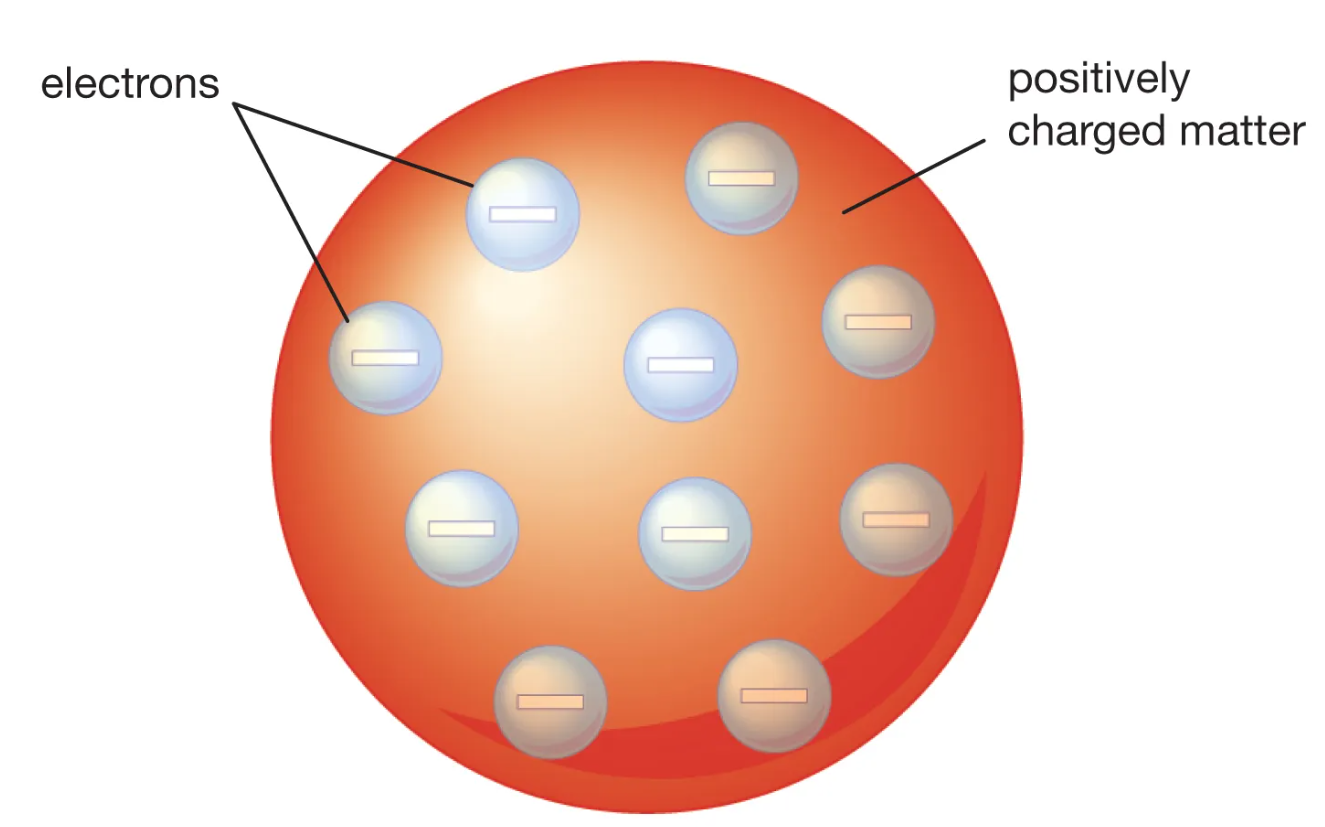
\includegraphics[trim={0 0  0 0cm} ,clip,width=.982\textwidth]{Introduction/plumb.png}
                        \caption{{Thomson model of atom, with negatively charged electrons embedded in positively charged ball \\
                        {\myfont{\tiny  [Britannica:Thomson Atomic Model]   }}}}
                        %britannica.com/science/Thomson-atomic-model
                        \label{fig:plumpudding}
                    \end{figure}
            
    \end{columns}
\end{frame}

%\begin{frame}{Introduction Notes}%
%Put in pictures of people - rutherford geiger marsden democritus jj thomson
%\end{frame}


\begin{frame}{Brief History of the Proton}


   \begin{columns}
        \column{0.69\textwidth}
        
              \begin{itemize}
                    \setlength\itemsep{1em}
                    \item  \textbf{$\sim$ 1911: Discovery of the Nucleus} - Scattering $\alpha$ particles off gold foil yielded significant backscatter, indicating small, dense nucleus  {\myfont{\tiny  [Wikipedia:Geiger-Marsden]   }}
                    \item \textbf{$\sim$ 1919: Discovery of the Proton} - Proposed by Rutherford after $\alpha$ particle scattering experiments off atoms {\myfont{\tiny  [E. Rutherford doi:10.1080/14786431003659230]   }}
                    \item \textbf{$\sim$1961: Discovery of Quarks} - Electron scattering experiments provided evidence consistent with the proton being a composite object of point-like constituents 
                    \end{itemize}

        \column{0.31\textwidth}
                    %\vspace{2cm}
                    \begin{figure}
                        \centering
                        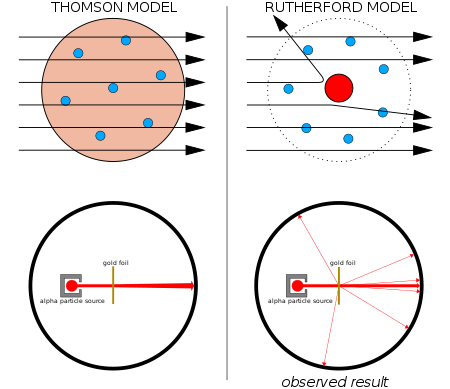
\includegraphics[trim={9cm 8cm  0 0cm} ,clip,width=.6\textwidth]{Introduction/rutherfordscattering.png}
                        \caption{     {\myfont{\tiny  [Wikimedia:Geiger-Marsden Exp.]   }}}
                        %https://upload.wikimedia.org/wikipedia/commons/thumb/8/89/Bohr_model_Hydrogen.svg/1280px-Bohr_model_Hydrogen.svg.png
                        \label{fig:plumpudding1}
                    \end{figure}
                    \vspace{-1cm}
                     \begin{figure}
                        \centering
                        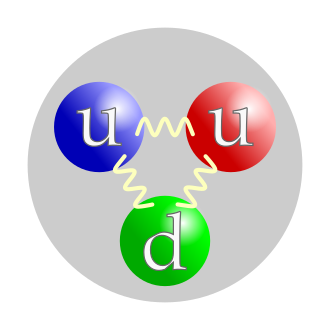
\includegraphics[trim={0 0  0 0cm} ,clip,width=.65\textwidth]{Introduction/proton_quarks.png}
                        \caption{
                        {\myfont{\tiny  [Wikimedia:Proton Quark Structure]   }}}
                        %https://upload.wikimedia.org/wikipedia/commons/thumb/8/89/Bohr_model_Hydrogen.svg/1280px-Bohr_model_Hydrogen.svg.png
                        \label{fig:plumpudding2}
                    \end{figure}
            
    \end{columns}
\end{frame}


\begin{frame}{The Proton is Now Well-Understood}
   \begin{columns}
        \column{0.69\textwidth}
        Protons are:
              \begin{itemize}
                    \setlength\itemsep{1em}
                    \item \textbf{Spin 1/2}
                    \item \textbf{Stable}: mean lifetime $>$ 1E34 years 
                    \item \textbf{Lightweight}: 938.272088 MeV; lightest baryon\\
                     {\myfont{\tiny  [n.b. 1 eV = 1.8E-36 kg]   }}
                    \item \textbf{Small}: radius $\sim$ 0.85 fm\\
                         \begin{itemize}
                            \item If protons were scaled to the size of pingpong balls,\\
                            atoms would be $\sim$ 4 football fields across,\\
                            humans would be $\sim$ diameter of the inner solar system
                        \end{itemize}
                    \end{itemize}
                    
                    
        \column{0.31\textwidth}
                    %\vspace{2cm}
                    \begin{figure}
                        \centering
                        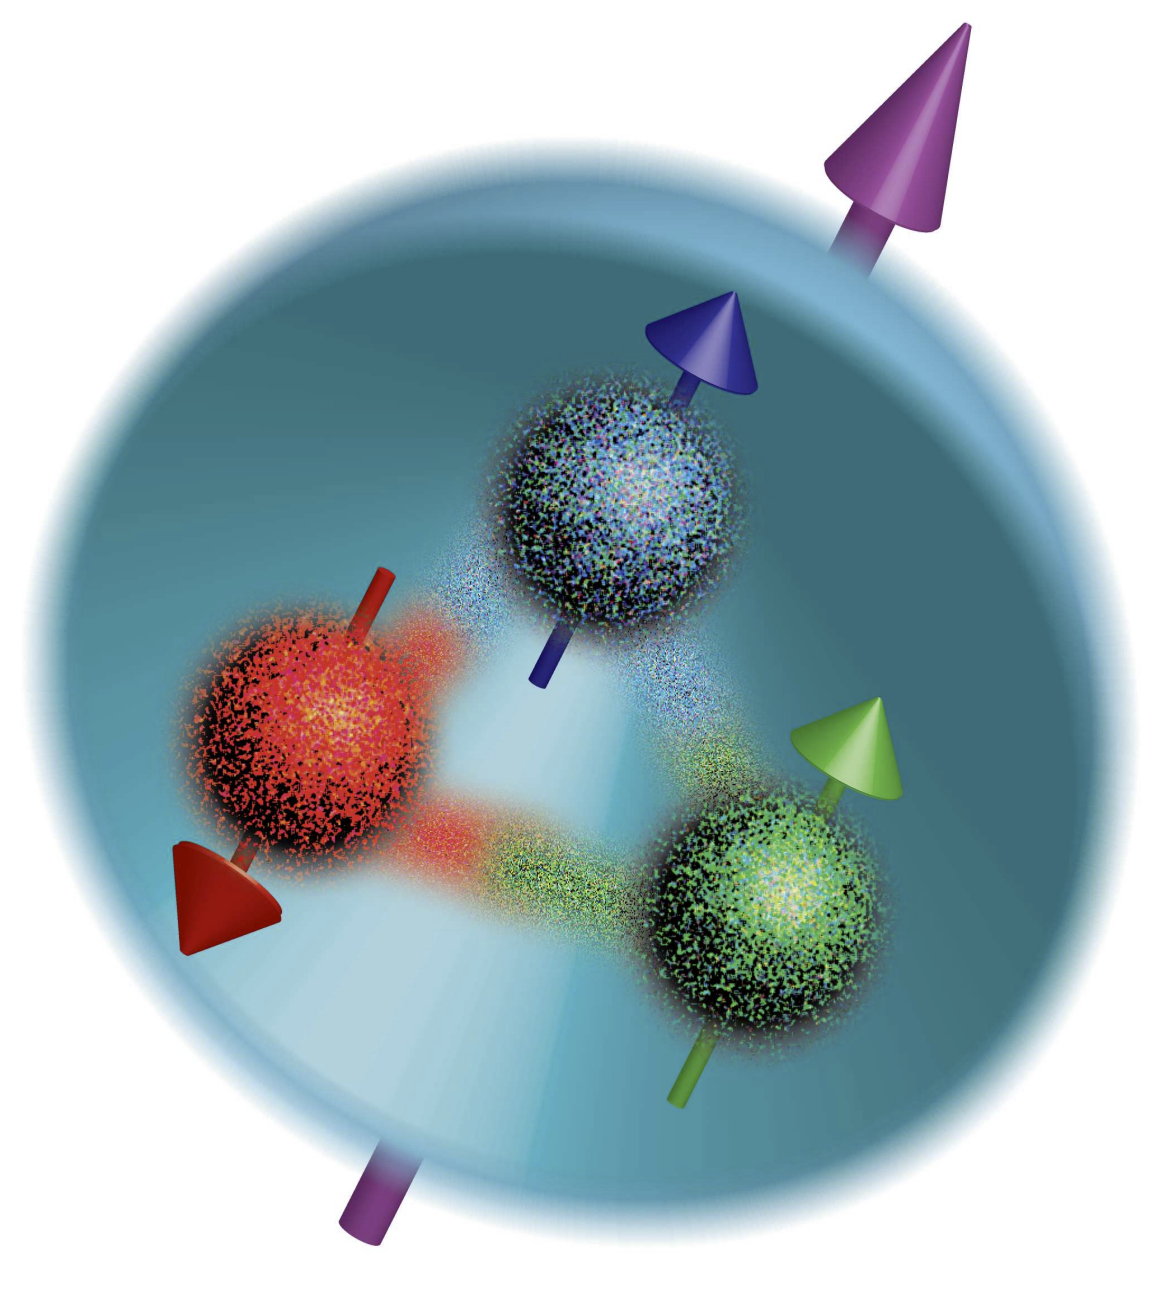
\includegraphics[trim={0 0  0 0cm} ,clip,width=.982\textwidth]{Introduction/eic_spin.png}
                        \caption{                       {\myfont{\tiny  [EIC Whitepaper]   }}}
                        %https://www.anl.gov/article/getting-up-to-speed-on-the-proton
                        \label{fig:modernproton1}
                    \end{figure}
            
    \end{columns}
\end{frame}


%\begin{frame}{What is a Pion}
%(quark constituents, show standard model particles, etc)
%\end{frame}

\begin{frame}{The Proton is \textbf{NOT YET} well-understood - Testbed for Physics}
    Macroscopic features are well measured, but many properties remain to be understood
    \begin{columns}

           \column{0.31\textwidth}
                    %\vspace{2cm}
                    \begin{figure}
                        \centering
                        %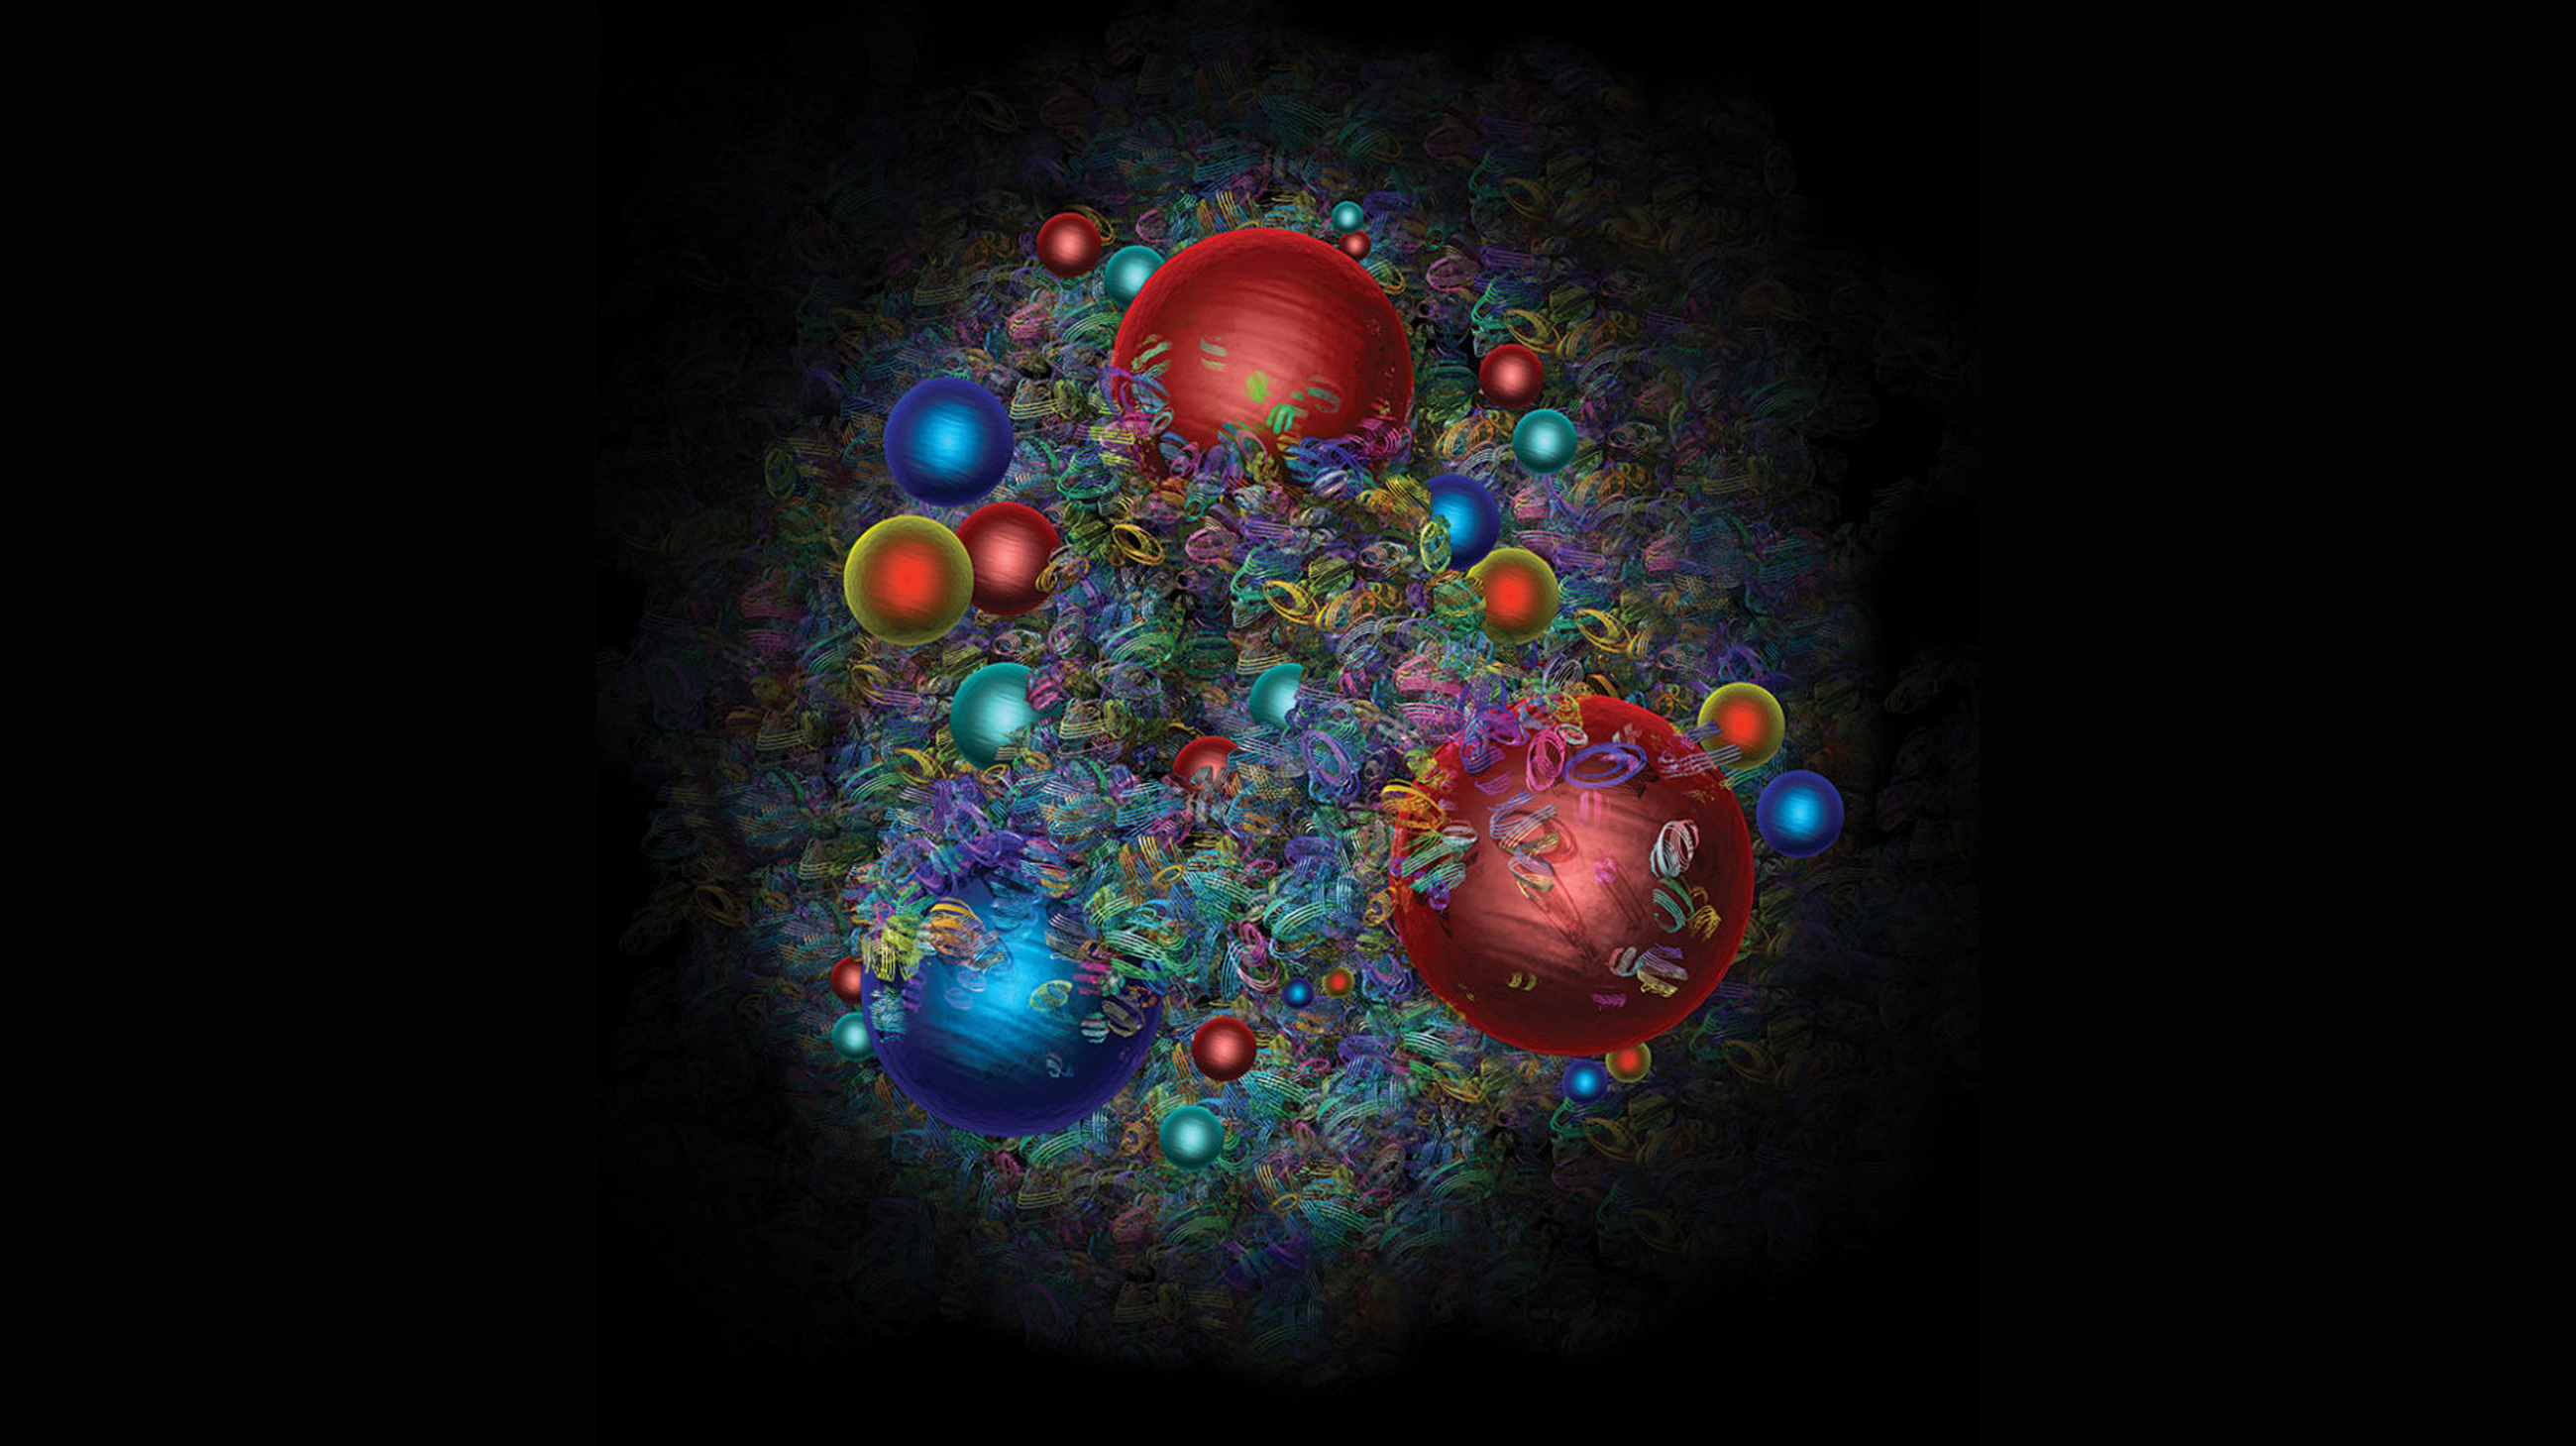
\includegraphics[trim={25cm 5cm  25cm 5cm} ,clip,width=.982\textwidth]{Introduction/quanta_protons.jpg}
                        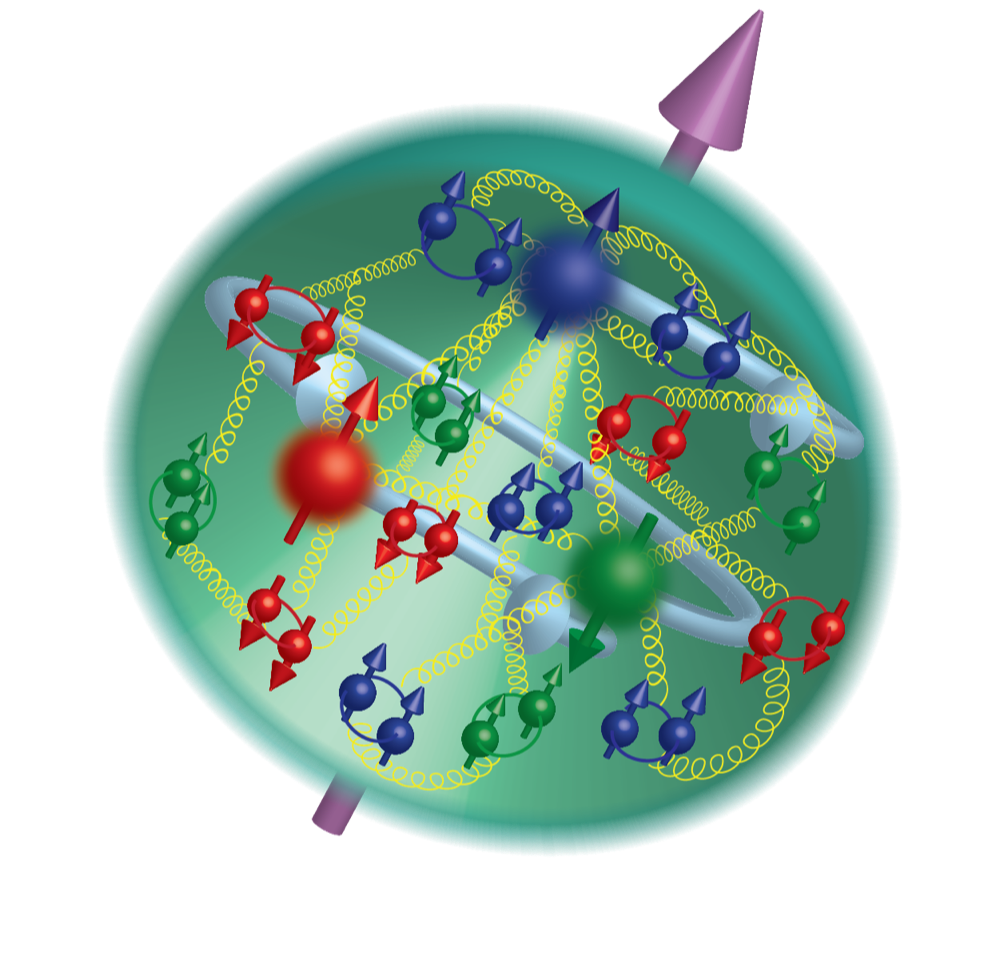
\includegraphics[trim={0 0  0 0cm} ,clip,width=.982\textwidth]{Introduction/modernproton.png}
                        \caption{                       {\myfont{\tiny  [Argonne National Lab]   }}}
                        %https://www.anl.gov/article/getting-up-to-speed-on-the-proton
                        \label{fig:modernproton2}
                    \end{figure}
                    
        \column{0.69\textwidth}
       
              \begin{itemize}
                    \setlength\itemsep{1em}
                     \item \textbf{Proton Spin Crisis}: Where does the proton's spin come from? 1987 measurement showed valence quarks only contribute  a small percent to overall proton spin
                     \item \textbf{Proton Decay}: Popular Beyond-Standard-Model theories predict the proton to decay, but never has been observed
                     \item \textbf{Proton Radius Puzzle}: (possibly resolved) discrepancy in proton charge radius between experimental methods
                      \end{itemize}

            \quad \quad \quad  {\myfont{\tiny \quad \quad \quad [Proton Puzzles, Nat Rev Phys, 2021]   }}
                
            
    \end{columns}
\end{frame}


\begin{frame}{Probing the Proton: Accelerators as Electron Femtoscopes}
Imaging limited by diffraction ($\sim \frac{\lambda}{2}$) $\rightarrow$ scale set by $\lambda = \frac{hc}{pc}$ with hc = 1200 eV nm
  \begin{columns}

           \column{0.33\textwidth}
                        %\vspace{2cm}
                       \centering 
                    \textbf{Optical Microscope}
                    \begin{figure}
                        \centering
                        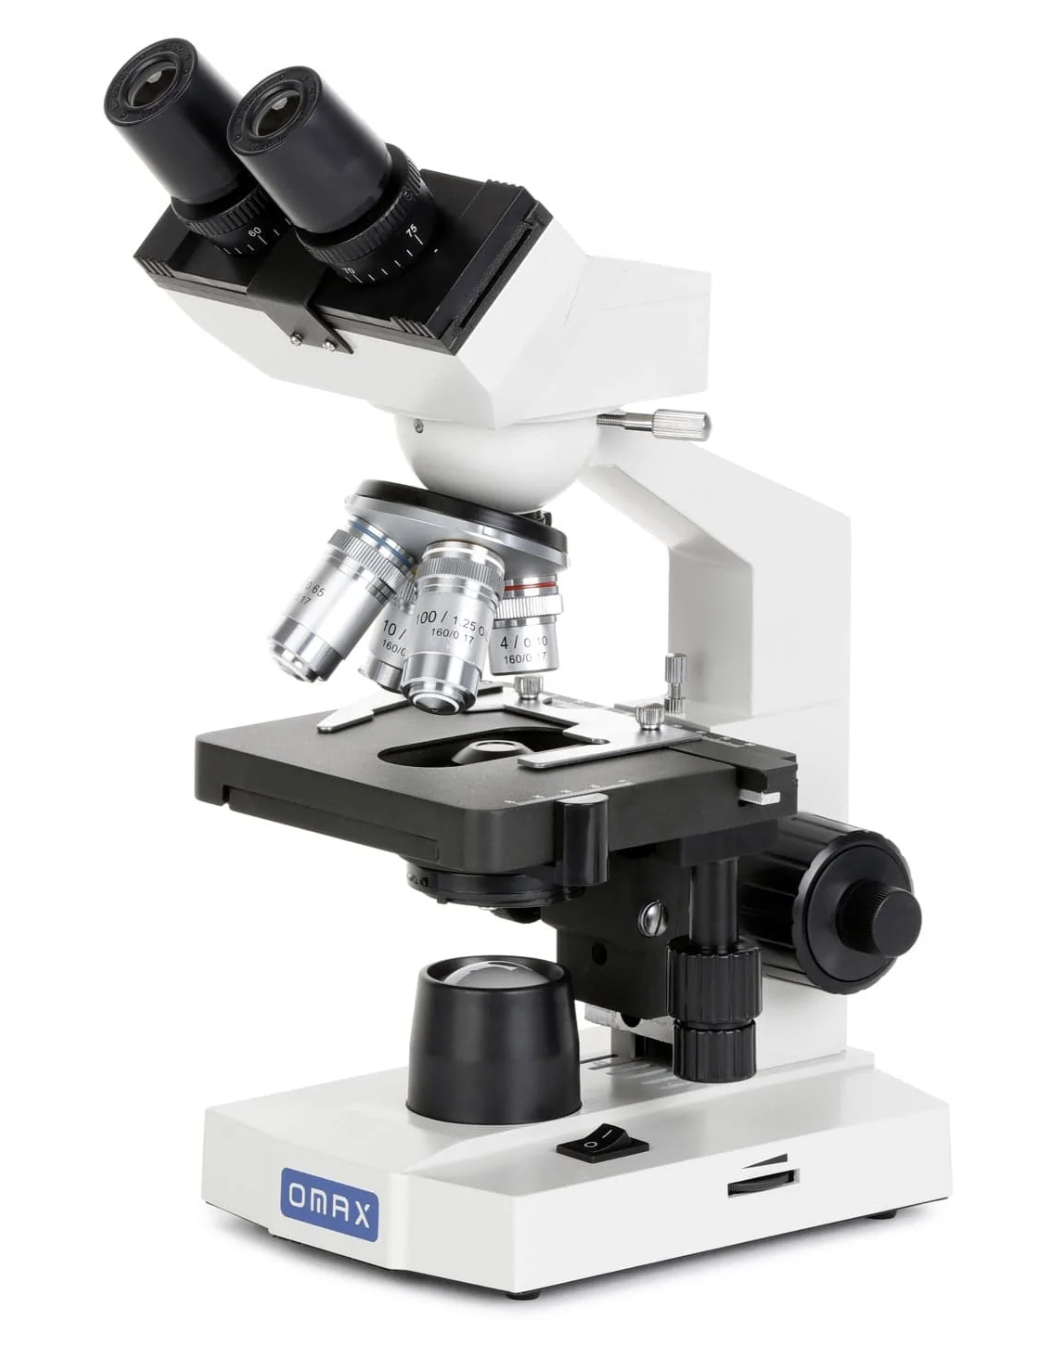
\includegraphics[trim={0 1cm 0 0cm} ,clip,width=.63\textwidth]{Introduction/optmic.png}
                        %\caption{                       {\myfont{\tiny  [Quanta Magazine 20190911]   }}}
                        %https://www.anl.gov/article/getting-up-to-speed-on-the-proton
                        \label{fig:modernproton3}
                    \end{figure} 
                     3 eV $\rightarrow$ $\lambda$ $\sim$ 400 nm\\
                     {\myfont{\tiny \quad \quad \quad [n.b. ex. mic for bio]   }}
        \column{0.33\textwidth}
        \centering
        \textbf{Electron Microscope}
                    \begin{figure}
                        \centering
                        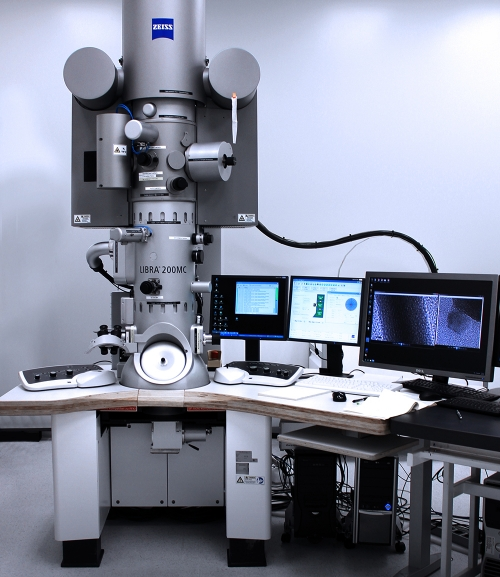
\includegraphics[trim={0 0 0 0} ,clip,width=.77\textwidth]{Introduction/elecmic.jpg}
                        %\caption{                       {\myfont{\tiny  [Quanta Magazine 20190911]   }}}
                        %https://www.anl.gov/article/getting-up-to-speed-on-the-proton
                        \label{fig:modernproton4}
                    \end{figure} 
             10 keV $\rightarrow$ $\lambda$ $\sim$ 0.01 nm
                    
         \column{0.33\textwidth}
         \centering
         \textbf{Electron Accelerator}
                    \begin{figure}
                        \centering
                        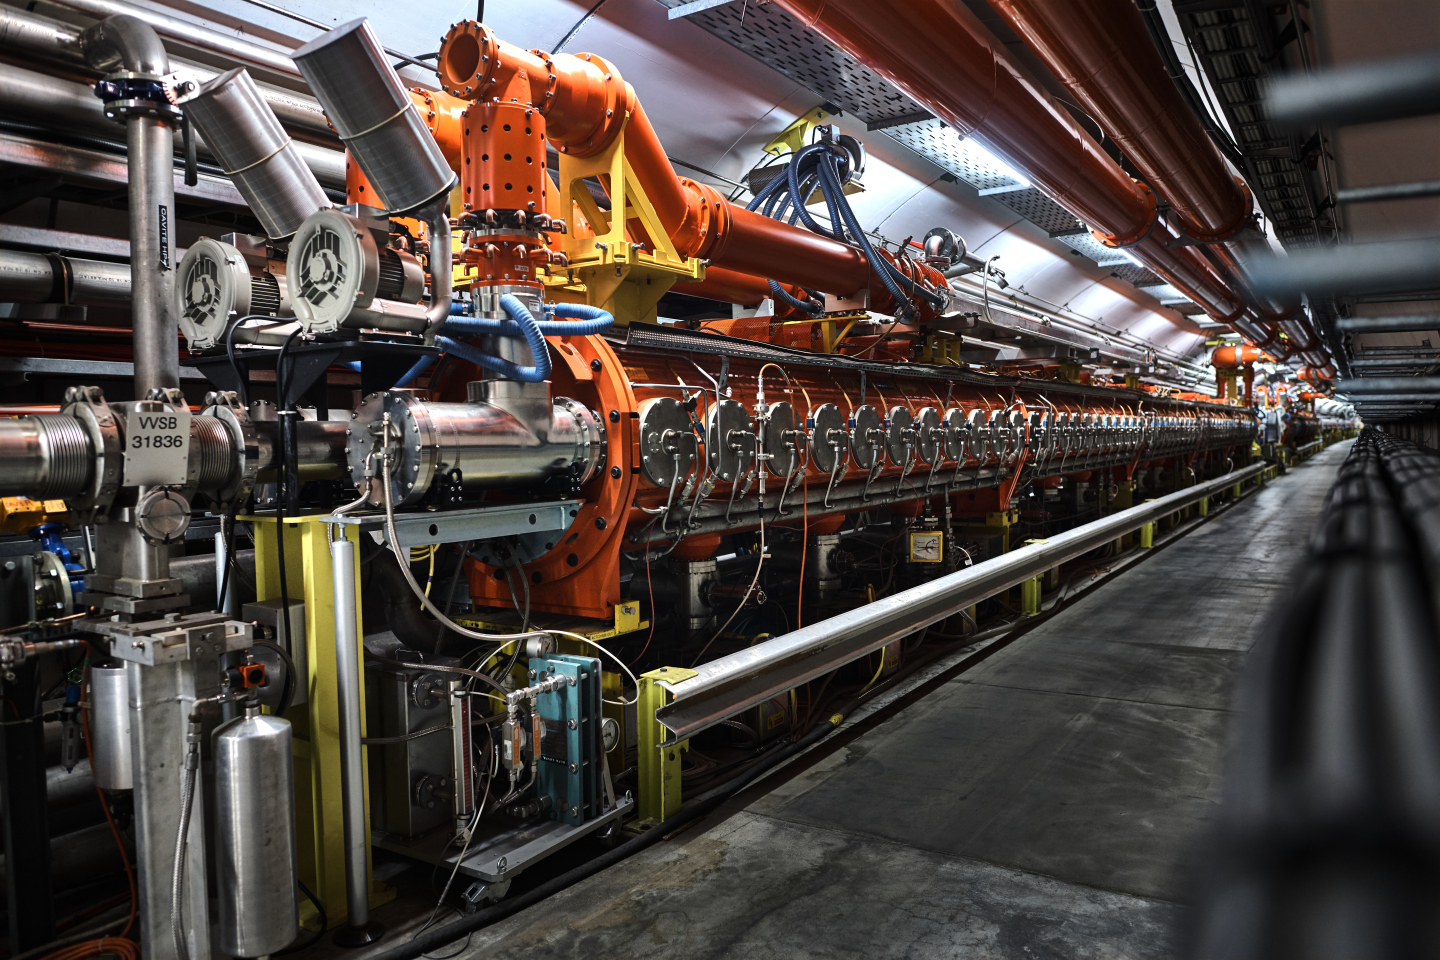
\includegraphics[trim={2cm 0 2cm 0} ,clip,width=.82\textwidth]{Introduction/elecfemt.jpg}
                        %\caption{                       {\myfont{\tiny  [Quanta Magazine 20190911]   }}}
                        %Source  https://home.cern/science/engineering/accelerating-radiofrequency-cavities
                    \end{figure} 
            10 GeV $\rightarrow$ $\lambda$ $\sim$ 0.1 fm
                    
         
    \end{columns}
\end{frame}

\begin{frame}{Proton Structure must be Indirectly Imaged}
Unlike optical imaging, must infer structure from reaction rates (cross sections) $\rightarrow$ structure encoded in various form factors and distribution functions
\begin{columns}

           \column{0.4\textwidth}
                \begin{figure}
                        \centering
                        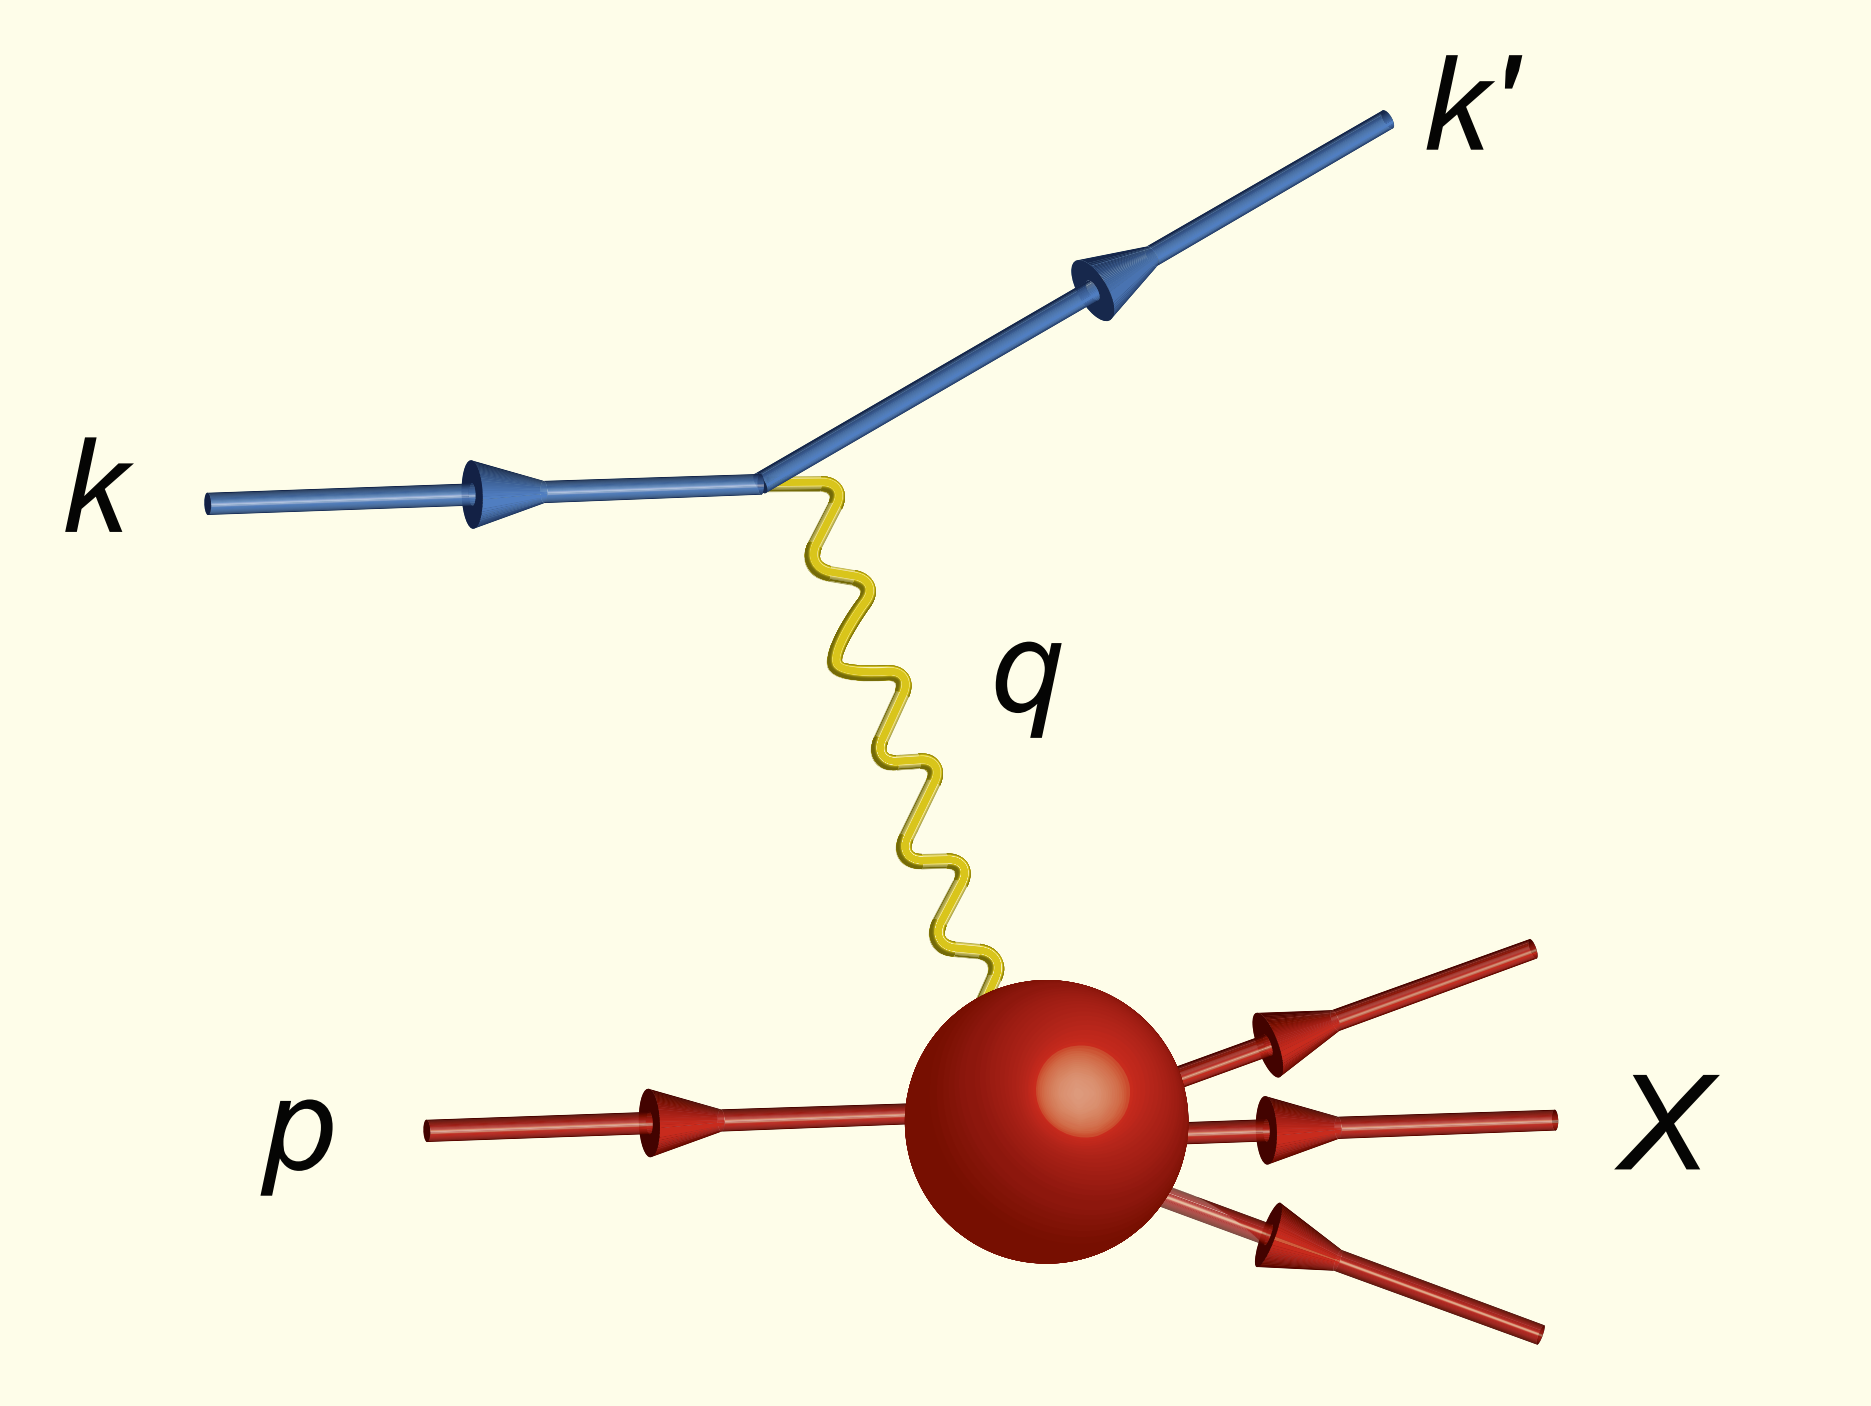
\includegraphics[trim={0cm 0 0cm 0} ,clip,width=.42\textwidth]{Introduction/gendia.png}
                        %\caption{                       {\myfont{\tiny  [Quanta Magazine 20190911]   }}}
                        %Source  https://home.cern/science/engineering/accelerating-radiofrequency-cavities
                         
                    \end{figure} 
                \vspace{-0.5cm}
                        \begin{figure}
                        \centering
                        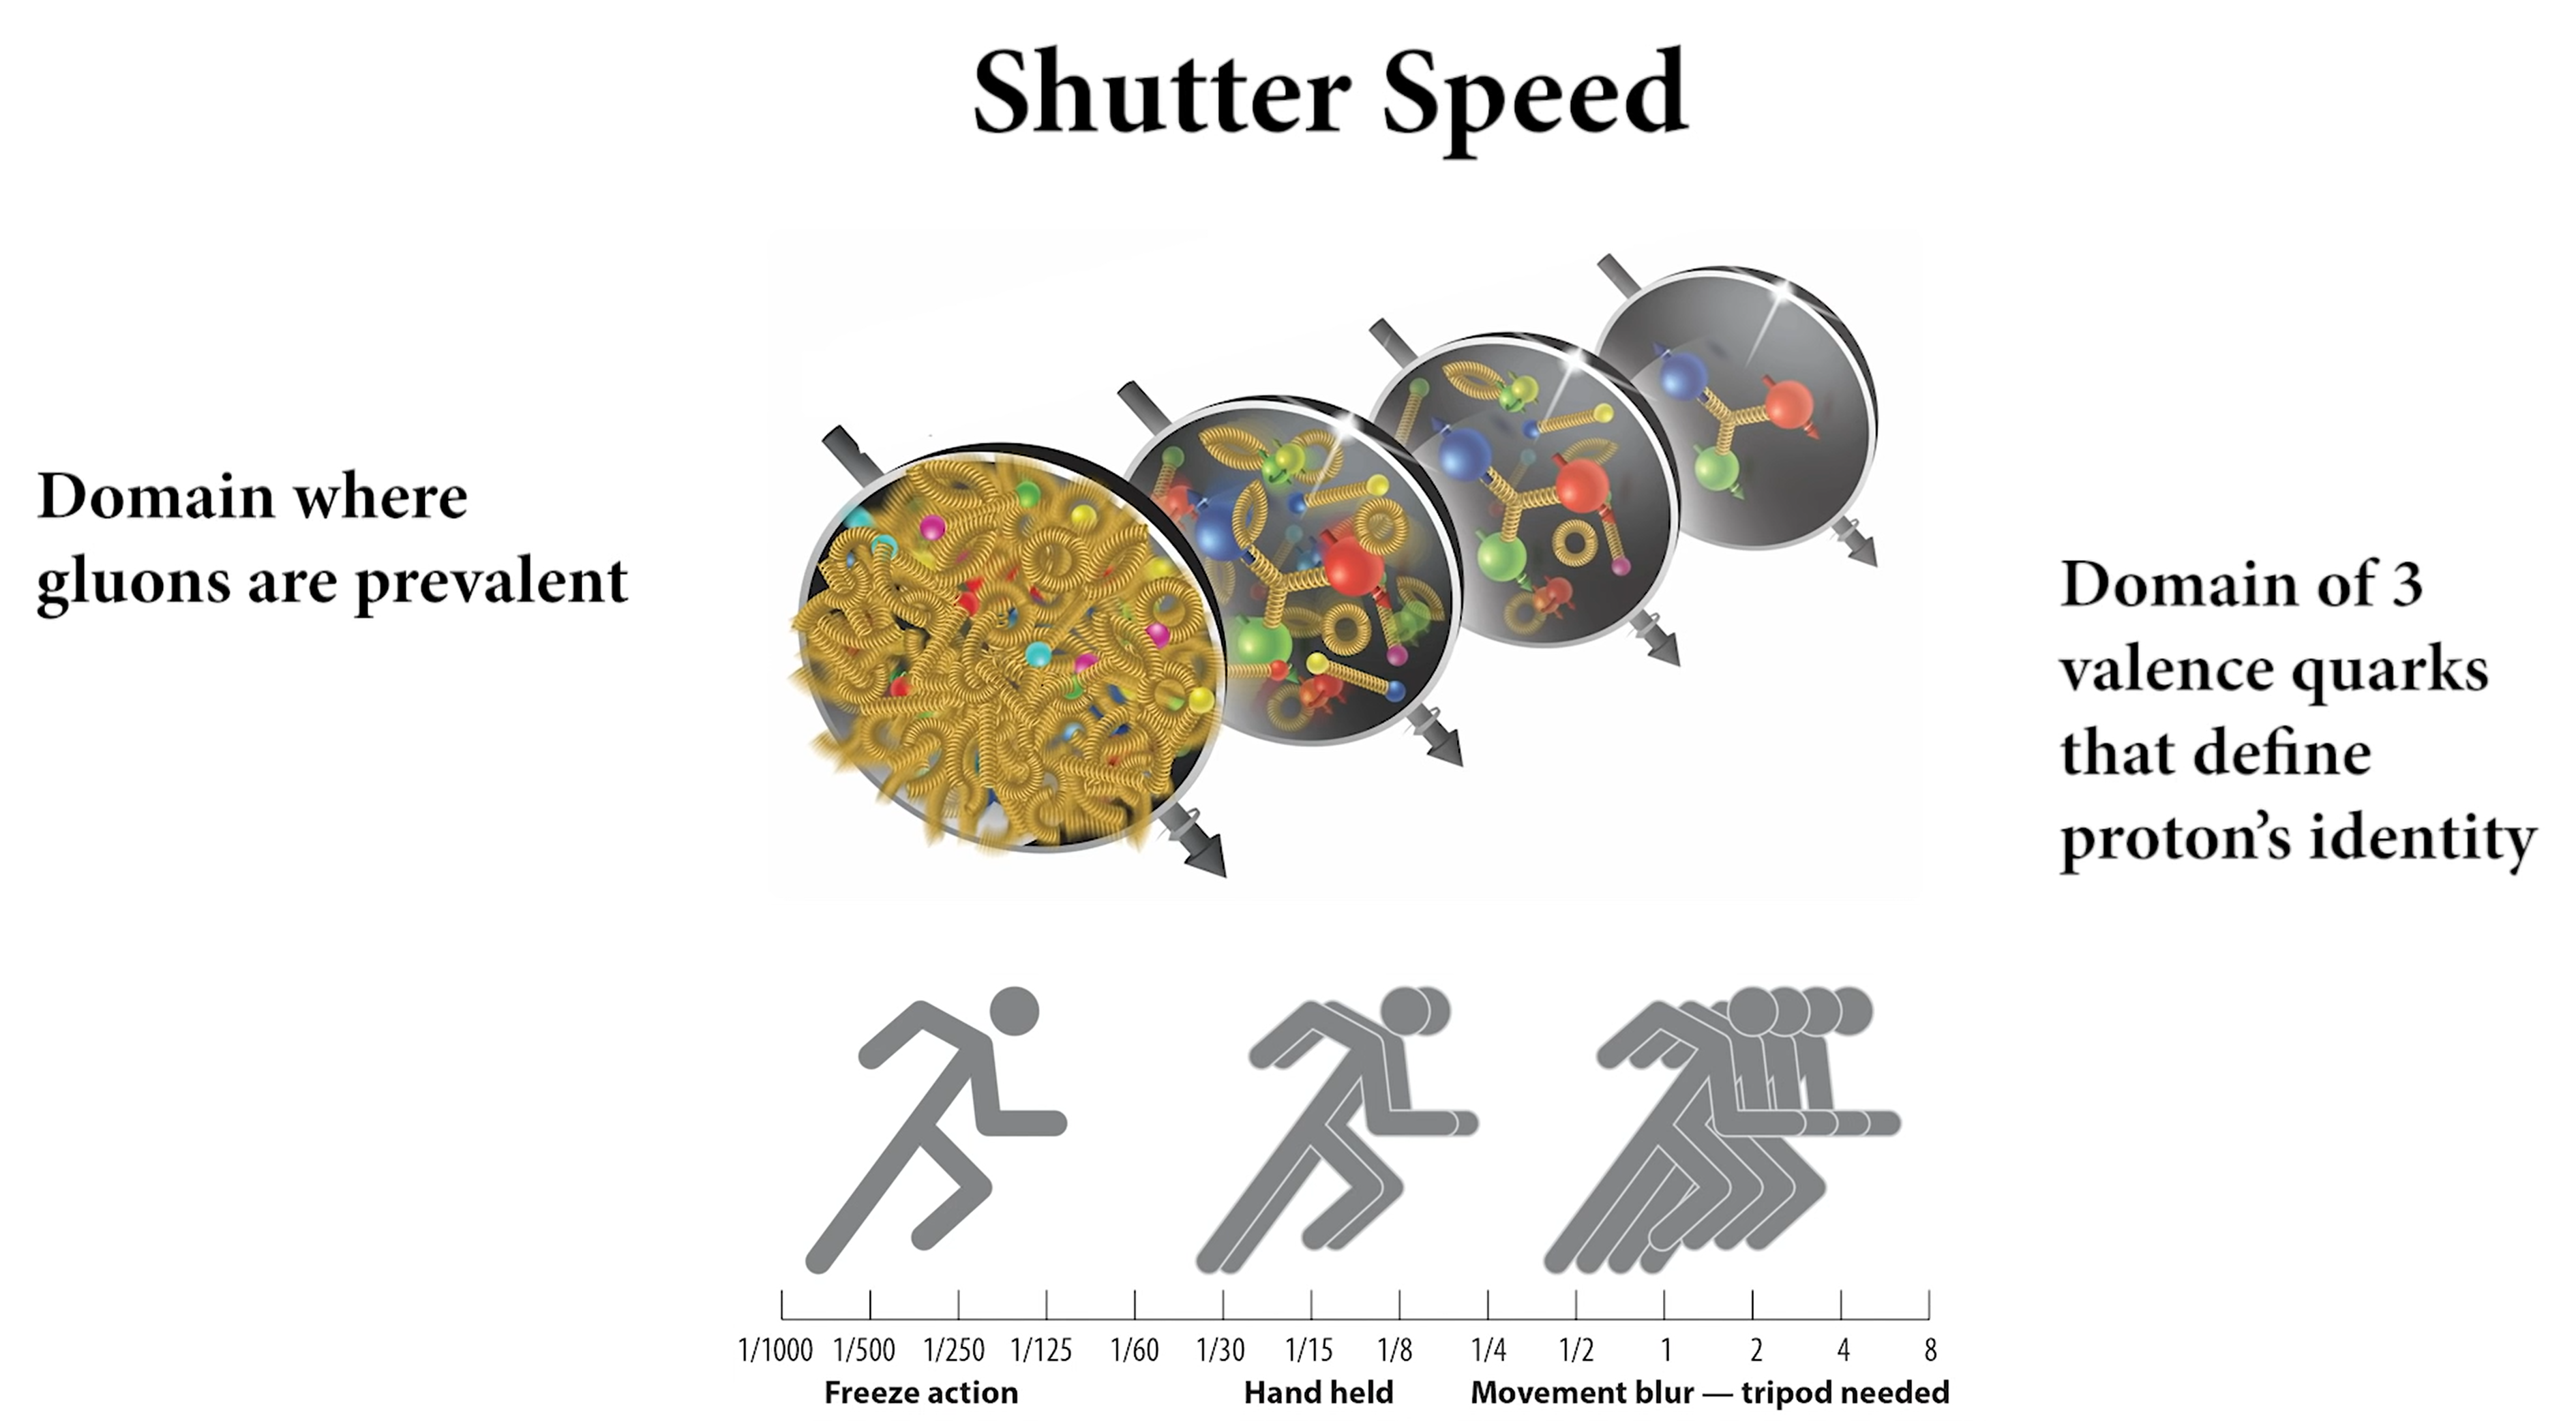
\includegraphics[trim={17cm 0 17cm 0} ,clip,width=.42\textwidth]{Introduction/shutter_speed.png}
                        \caption{                       {\myfont{\tiny  [R.G. Milner and R. Ent, \\
                        Visualzing the Proton (2022)]   }}}
                        %Source  https://home.cern/science/engineering/accelerating-radiofrequency-cavities
                         
                    \end{figure} 
      \column{0.6\textwidth}              

    \begin{itemize}
        \item Reactions of the form e + p $\rightarrow$ e + X
                \begin{itemize}
                \item X = p: elastic scattering
                \item X = X: inclusive scattering
                \item X = p + $\pi$: DV$\pi$P (in proper kinematic regime)
                \end{itemize}
        \item   $\frac{1}{q}$ determines the spatial resolution
                    
        \item $\frac{1}{x_B}$ determines the shutter speed
        
    \end{itemize}
    \vspace{-.5cm}
\begin{figure}
                        \centering
                        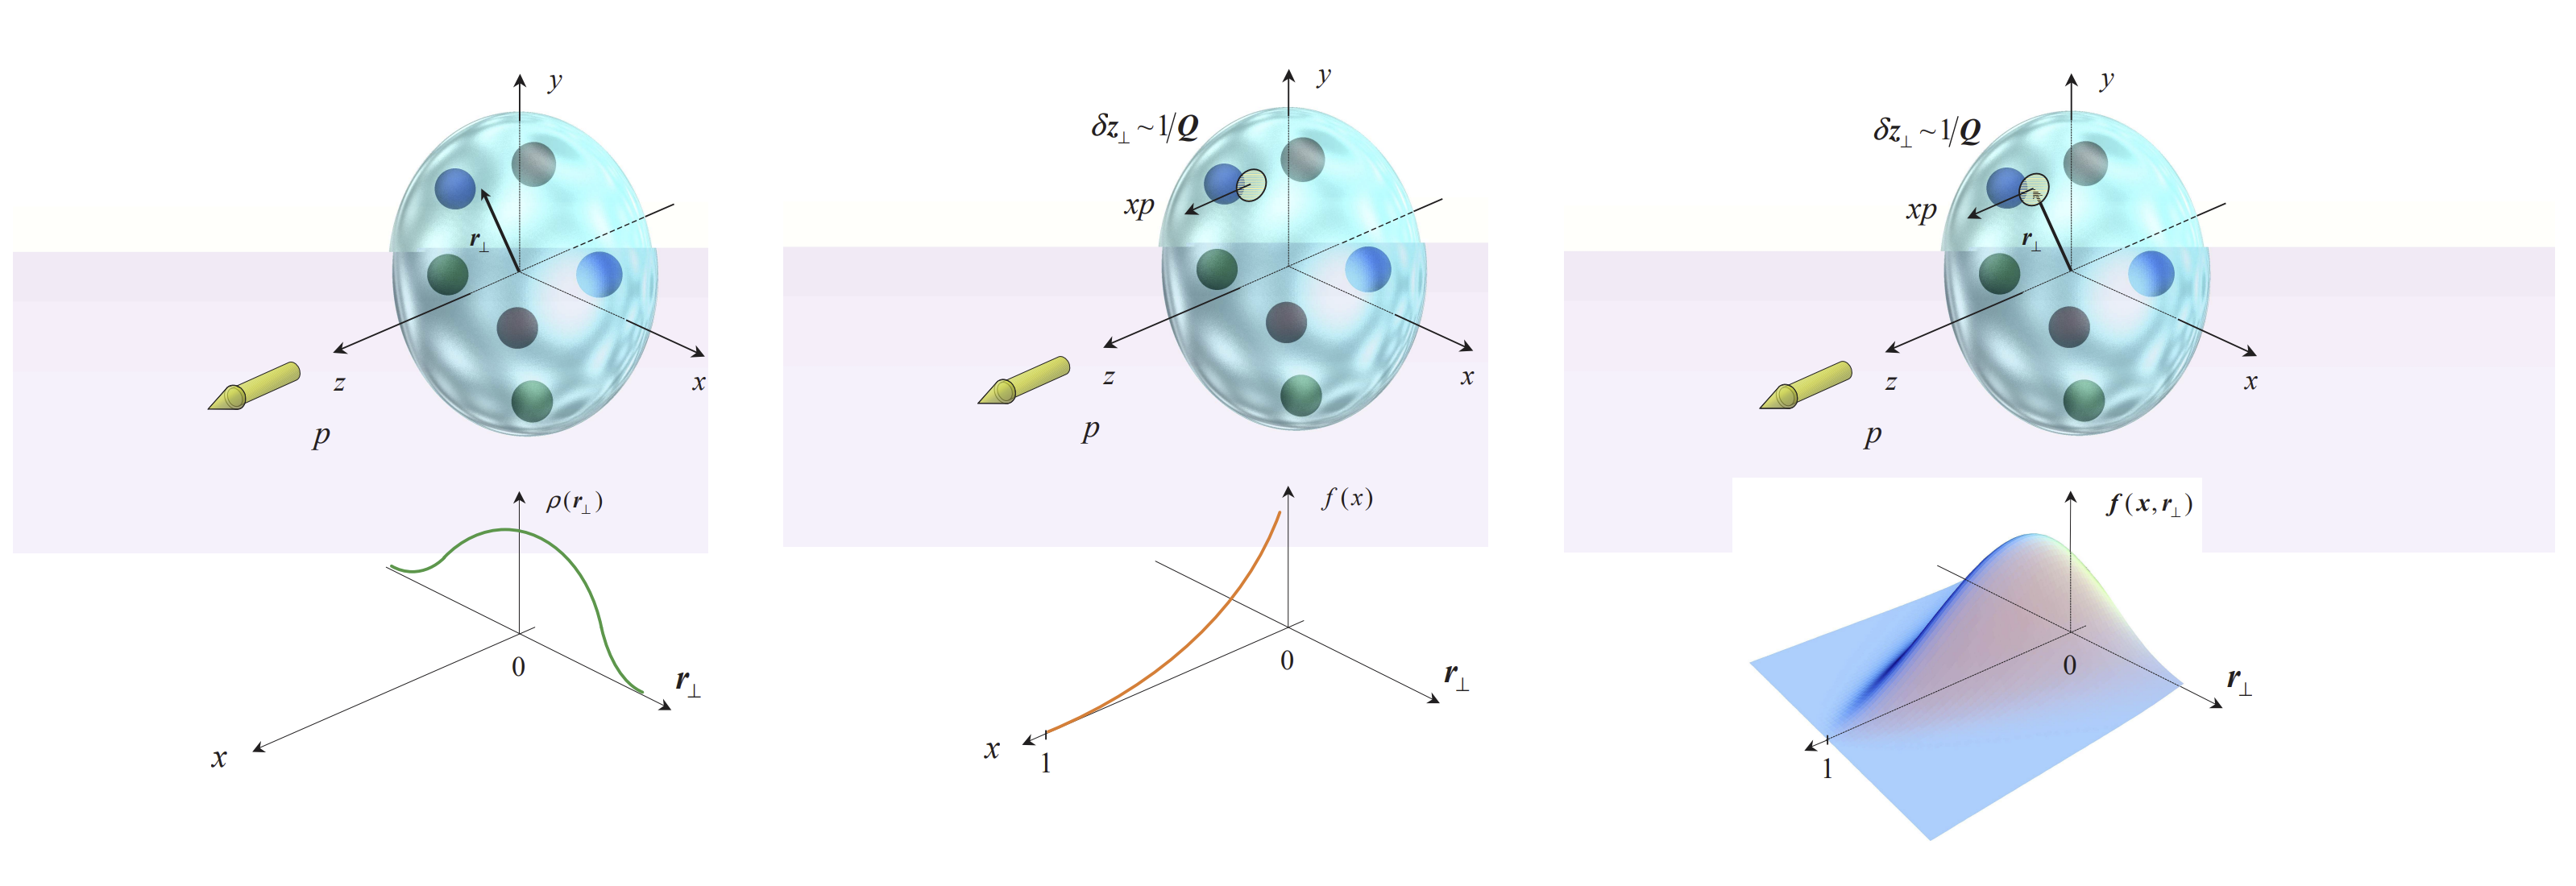
\includegraphics[trim={5cm 0 5cm 0} ,clip,width=.62\textwidth]{Introduction/ff_pdf_gpd.png}
                        \caption{                       {\myfont{\tiny  [A.V. Belitsky A.V. Radyushkin 2005]   }}}
                        %Source  https://home.cern/science/engineering/accelerating-radiofrequency-cavities
                         
                    \end{figure} 

    \end{columns}
\end{frame}


\begin{frame}{GPDs Encode Proton 3D Structural Information}

\begin{columns}

           \column{0.4\textwidth}

                        \centering
                        Proton Form Factors
                        \vspace{-.1cm}
                                                     \begin{figure}
                        \centering
                        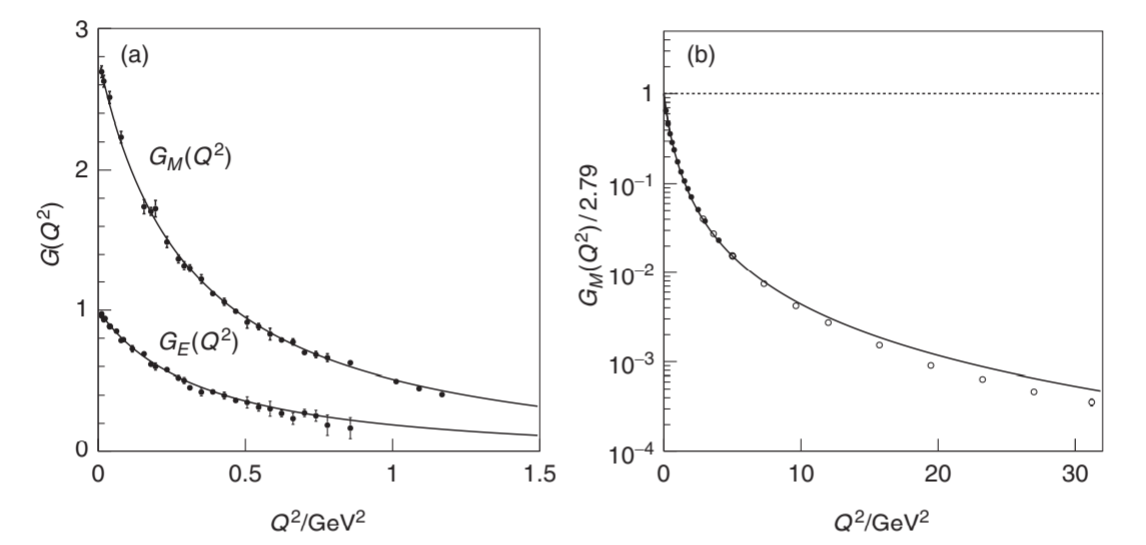
\includegraphics[trim={0 0 0 0} ,clip,width=.82\textwidth]{Introduction/rosenbluth-2.PNG}
                        %\caption{Proton From Factors}
                        %\caption{                       {\myfont{\tiny  [Quanta Magazine 20190911]   }}}
                        %Source  https://home.cern/science/engineering/accelerating-radiofrequency-cavities
                         
                    \end{figure}    
                    \vspace{-.5cm}
                 \begin{figure}
                        \centering
                        Parton Distribution Functions
                        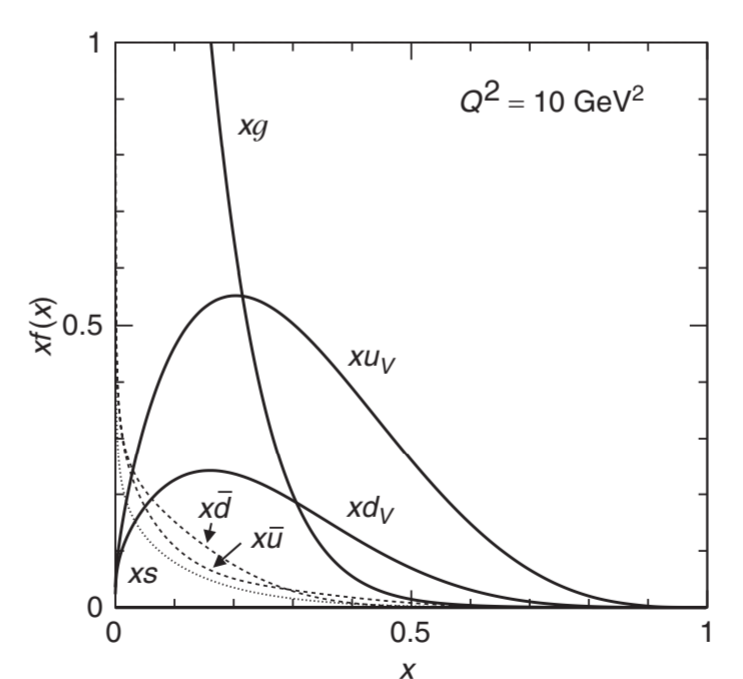
\includegraphics[trim={0 0 0 0} ,clip,width=.562\textwidth]{Introduction/pdf-10gev.PNG}
                        %\caption{Parton Distribution Function at $Q^2=10GeV^2$}
                        %\caption{                       {\myfont{\tiny  [Quanta Magazine 20190911]   }}}
                        %Source  https://home.cern/science/engineering/accelerating-radiofrequency-cavities
                         
                    \end{figure} 

            \column{0.6\textwidth}

            %\centering
            \begin{itemize}
                \item All distribution functions related through limiting cases of Wigner distributions
                \item Quark and gluon Wigner distributions have no known direct physical observable
                \item Can experimentally access TMDs and GPDs
            \end{itemize}
            
                \begin{figure}
                        \centering
                        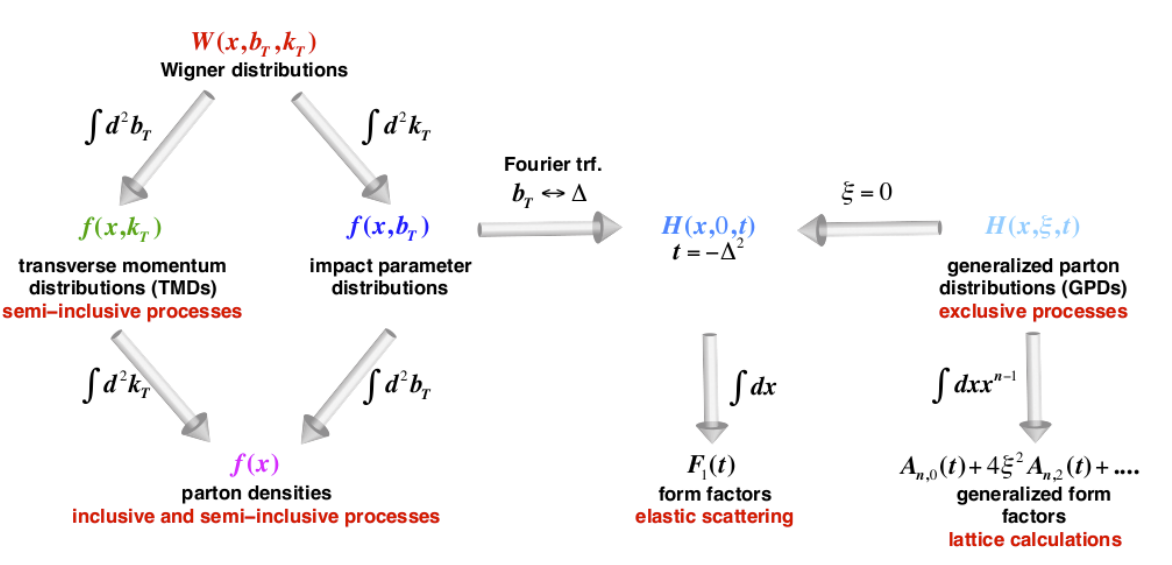
\includegraphics[trim={0 0 0 0} ,clip,width=.72\textwidth]{Introduction/wigner_cube.png}
                        \caption{ Relationships between different distribution functions\\
                        {\myfont{\tiny  [EIC Whitepaper]   }}}
                        %Source  https://home.cern/science/engineering/accelerating-radiofrequency-cavities
                         
                    \end{figure} 

                    
    \end{columns}

\end{frame}




\begin{frame}{GPDs Accessible Through Deeply Virtual Processes}
\begin{itemize}
    \item Deeply Virtual Processe (DVCS, DVMP)s: target nucleon remains intact, DIS regime
    \item Relies on factorization between hard scattering and soft QCD vertices
    \item Factorization proved rigorously for DVCS in Bjorken limit, for DVMP with longitudinally polarized photons (sufficient if dominates)
\end{itemize}


                \begin{figure}
                        \centering
                        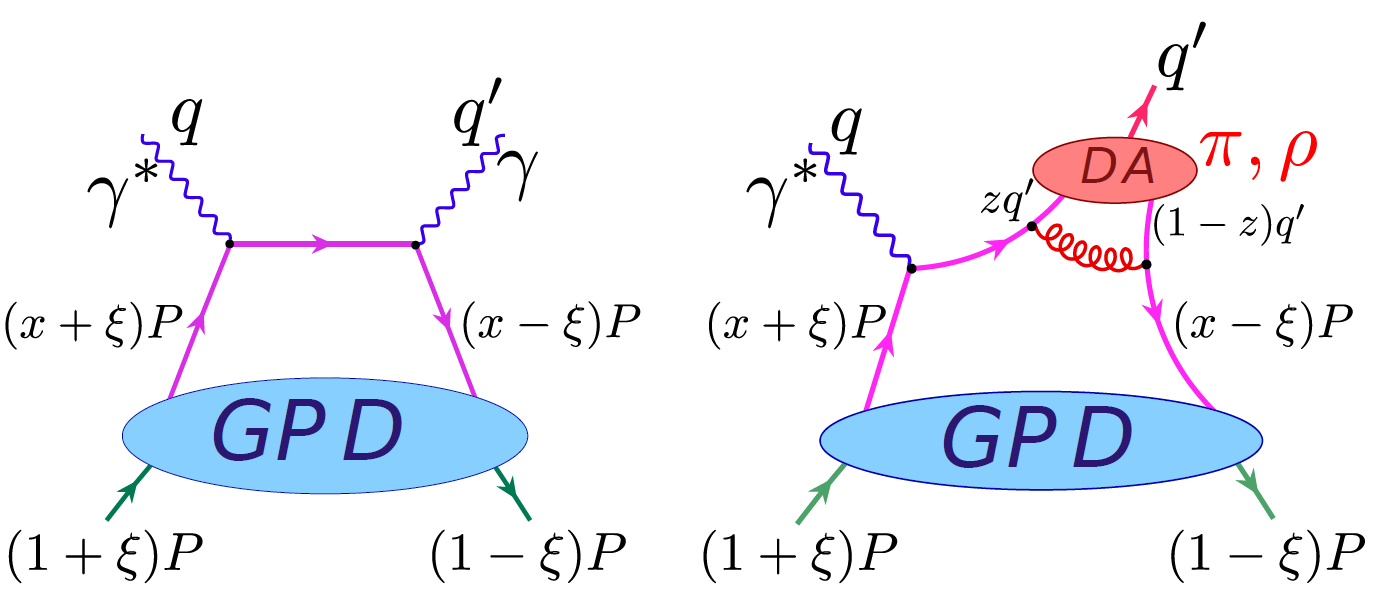
\includegraphics[trim={0 0 0 0} ,clip,width=.582\textwidth]{Introduction/andrey.png}
                        \caption{ DVCS (left) and DVMP Feynman Handbag diagrams\\
                        {\myfont{\tiny  [V. Kubarovsky Nuc Phys B 2011]   }}}
                        %Source  https://home.cern/science/engineering/accelerating-radiofrequency-cavities
                         
                    \end{figure} 
\end{frame}


\begin{frame}{Early Insights from Deeply Virtual Processes}
\begin{itemize}
    \item Deeply Virtual Processe (DVCS, DVMP)s: target nucleon remains intact, DIS regime
    \item Relies on factorization between hard scattering and soft QCD vertices
    \item Factorization proved rigorously for DVCS in Bjorken limit, for DVMP with longitudinally polarized photons (sufficient if dominates)
\end{itemize}

\begin{columns}
       \column{0.5\textwidth}

         \begin{figure}
                        \centering
                        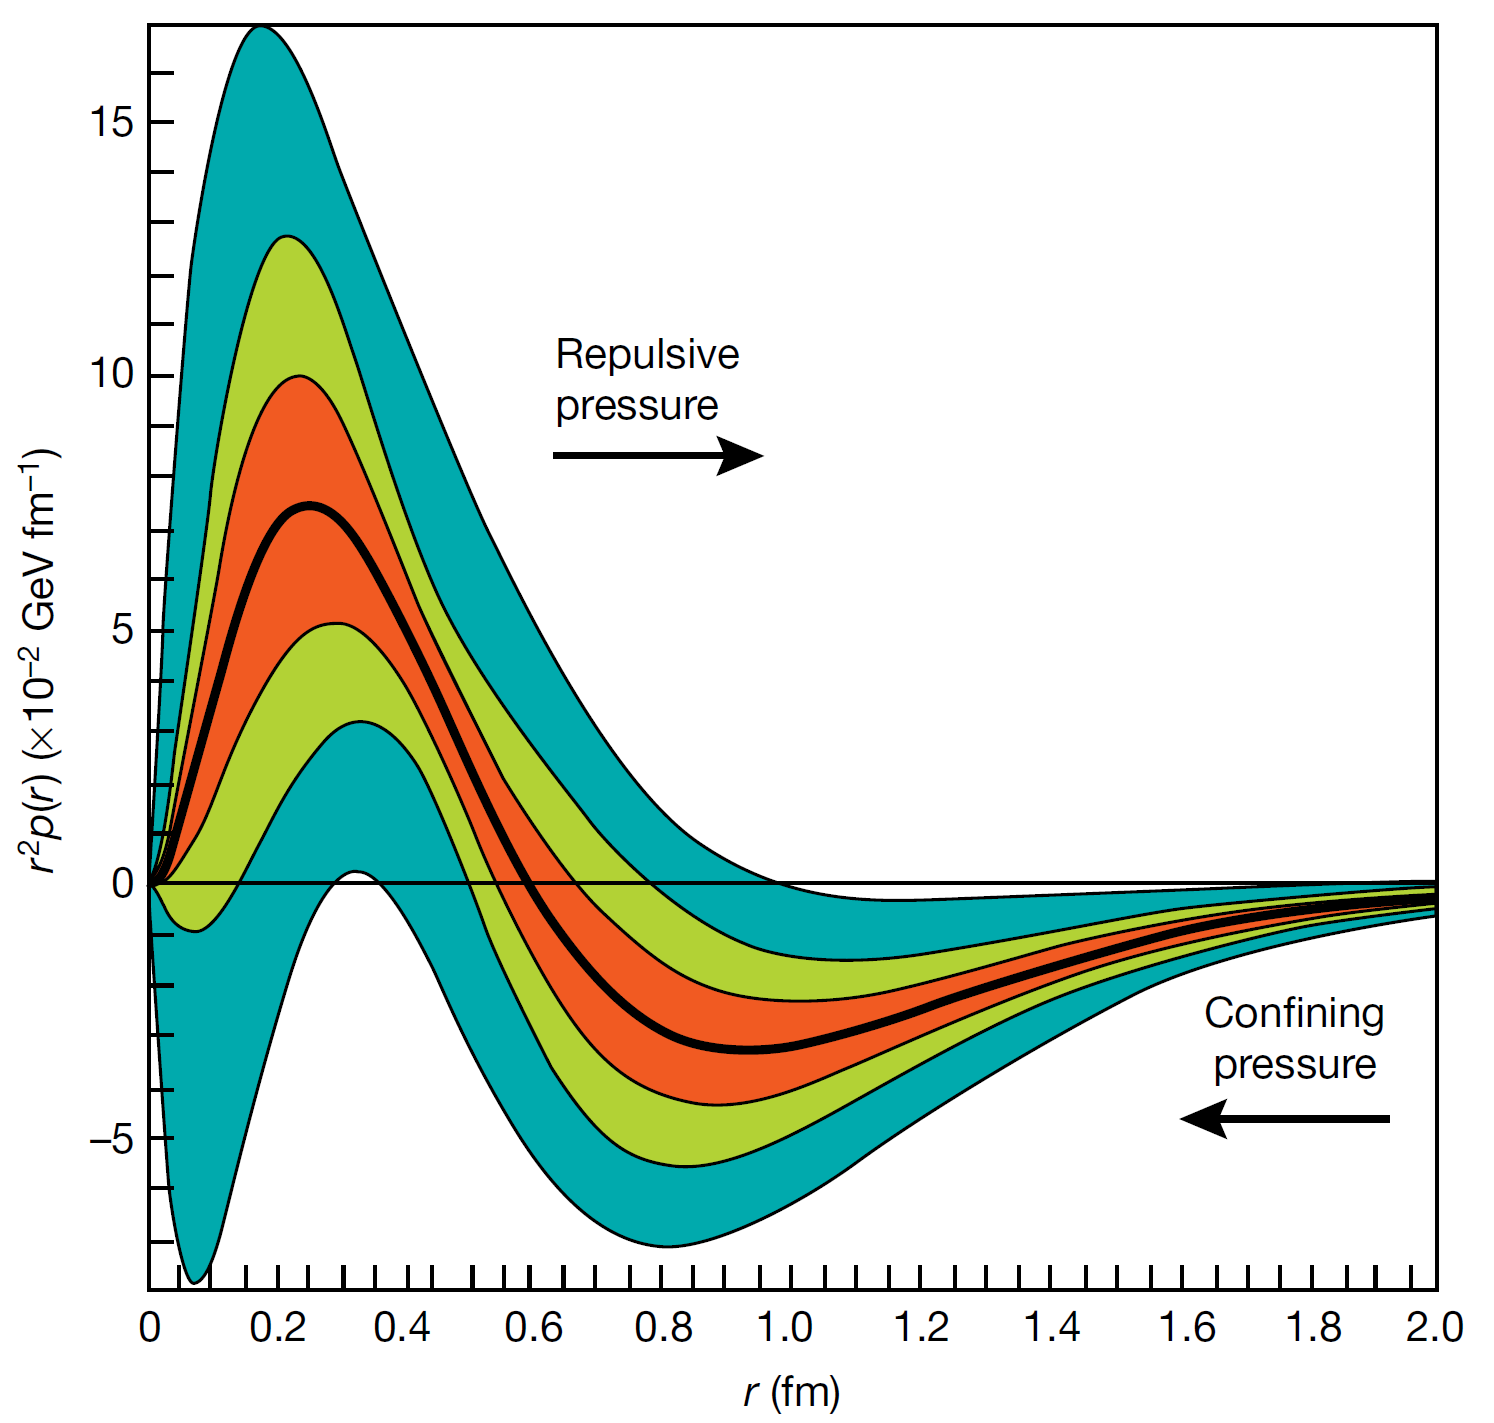
\includegraphics[width=.5\textwidth]{defense/proton_pressure_dist.png}
                      
                        \caption{ DVCS (left) and DVMP Feynman Handbag diagrams\\
                        {\myfont{\tiny  [V. Kubarovsky Nuc Phys B 2011]   }}}
                        %Source  https://home.cern/science/engineering/accelerating-radiofrequency-cavities
                         
                    \end{figure} 
       \column{0.5\textwidth}

         \begin{figure}
                        \centering
                       
                        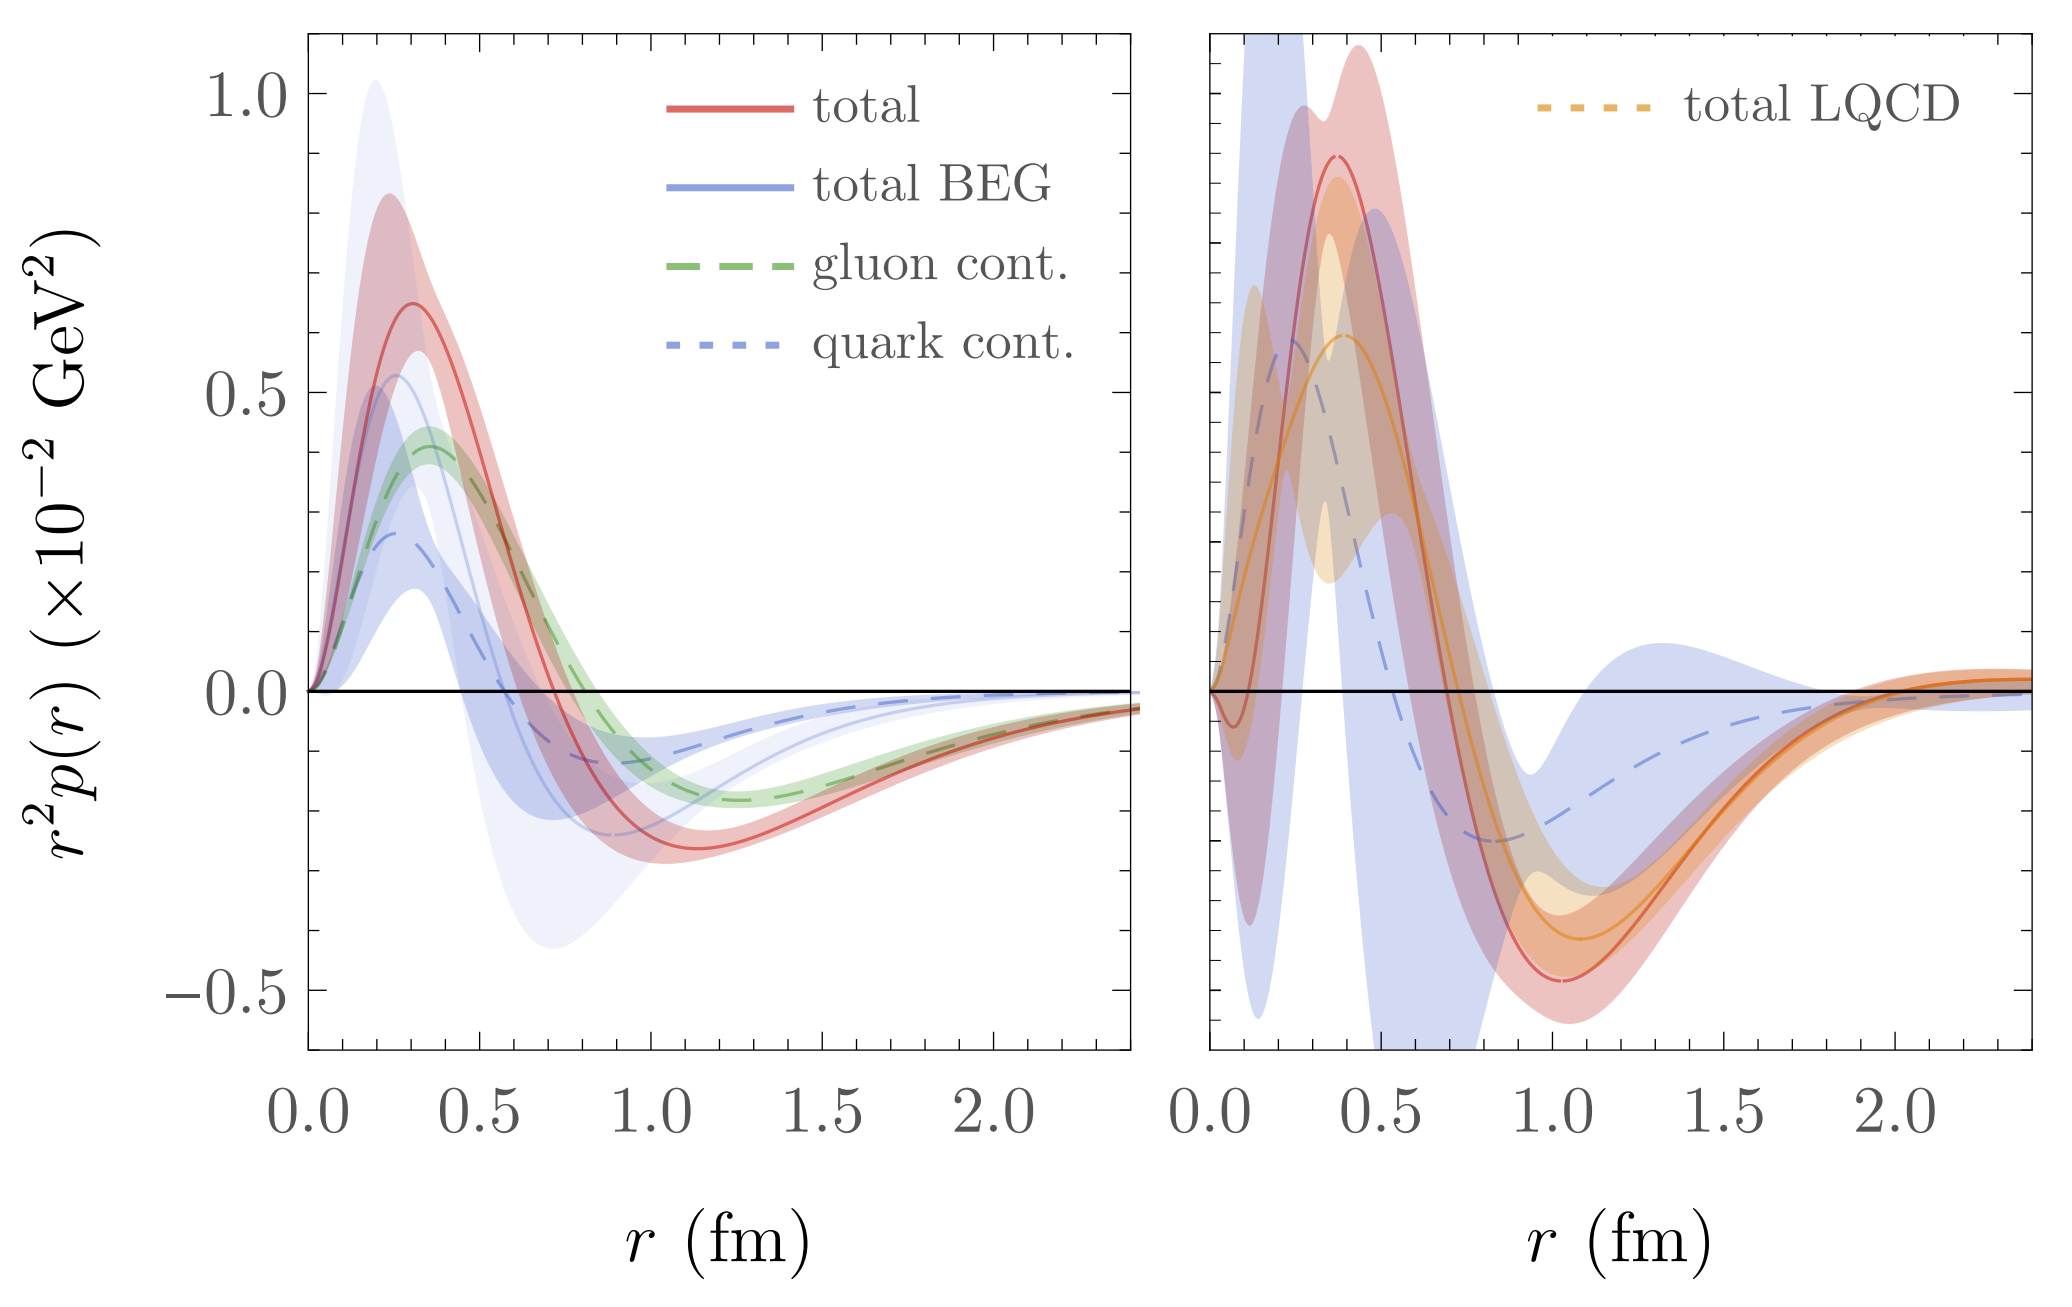
\includegraphics[width=.95\textwidth]{defense/proton_pressure_theory.png}
                        \caption{ DVCS (left) and DVMP Feynman Handbag diagrams\\
                        {\myfont{\tiny  [V. Kubarovsky Nuc Phys B 2011]   }}}
                        %Source  https://home.cern/science/engineering/accelerating-radiofrequency-cavities
                         
                    \end{figure} 
       
\end{columns}


\end{frame}



\begin{frame}{GPD Encoding in  $DV\pi^0P$ Cross Section is Nontrivial}

        \vspace{-.01cm}
   
    The cross section for DV$\pi^0$P can be expressed in terms of structure functions, which can be expressed as convolutions of GPDs:\\
    \vspace{0.1cm}
    \scalebox{0.735}{%
        $     \frac{d^4\sigma_{\gamma^*p \rightarrow p'\pi^0}}{dQ^2dx_Bdtd\phi_{\pi}} =
             \Gamma (Q^2, x_B, E)
             \frac{1}{2\pi}
             \left\{ \left(  \textcolor{sigmaT}{\frac{d\sigma_T}{dt}}+\epsilon  \textcolor{sigmaL}{\frac{d\sigma_L}{dt}} \right)+
             \epsilon cos(2\phi)  \textcolor{sigmaTT}{\frac{d\sigma_{TT}}{dt}} + 
             \sqrt{2\epsilon(1+\epsilon)} cos(\phi)  \textcolor{sigmaLT}{\frac{d\sigma_{LT}}{dt}} \right\}
             \quad | \quad
             \Gamma (Q^2, x_B, E) = \frac{\alpha}{8\pi} \frac{Q^2}{m^2_pE^2}\frac{1-x_B}{x_B^3}\frac{1}{1-\epsilon}$
    }
    %\vspace{0.05cm}

    \begin{columns}
       \column{0.5\textwidth}
    
            \begin{center}
                 The structure functions can be expressed in terms of GPDs:
            \end{center}
            
             \scalebox{0.80}{%   
            $      \textcolor{sigmaL}{\frac{d\sigma_{L}}{dt}} = 
            \frac{4\pi\alpha}{kQ^2}\left\{ \left( 1 - \xi^2 \right) 
            \lvert \langle \GPDHtildeEQ \rangle \rvert ^2 
            -2\xi^2 \Re \left[  \langle \GPDHtildeEQ \rangle ^* \langle \GPDEtildeEQ \rangle    \right] - \frac{t'}{4m^2}\xi^2
            \lvert \langle \GPDEtildeEQ \rangle \rvert ^2  \right\}$
            }\\
            
            \scalebox{0.80}{%   
            $      \textcolor{sigmaT}{\frac{d\sigma_{T}}{dt}} = 
            \frac{2\pi\alpha \mu_{\pi}^2}{kQ^4}
            \left\{ \left( 1 - \xi^2 \right) 
            \lvert \langle \GPDHTEQ \rangle \rvert ^2
            - \frac{t'}{8m^2}
            \lvert \langle \GPDETbarEQ \rangle \rvert ^2  \right\}$
            }\\
            
            \scalebox{0.80}{%   
            $     \textcolor{sigmaLT}{\frac{d\sigma_{LT}}{dt}} = 
            \frac{4\pi\alpha \mu_{\pi}}{\sqrt{2}kQ^3}
            \xi\sqrt{1-\xi^2}
            \frac{\sqrt{-t'}}{2m}
            \Re \left\{ 
             \langle \GPDHTEQ \rangle ^*
            \langle \GPDEtildeEQ \rangle   
            \right\}$
            }\\
        
            \scalebox{0.80}{%   
            $      \textcolor{sigmaTT}{\frac{d\sigma_{TT}}{dt}} = 
            \frac{4\pi\alpha \mu_{\pi}^2}{kQ^4}
            \frac{-t'}{16m^2}
            \langle \GPDETbarEQ \rangle^2   
            $
            }\\
           


        \column{0.5\textwidth}
    
            \centering 
            %\vspace{0.3cm}
            GPD Classification:\\\tiny{\textcolor{white}{lll}}\\
                 %\vspace{0.1cm}
                 \footnotesize
                 \begin{table}[H]
                    \centering
                    \begin{tabular}{@{} *{4}{c} @{}}
                        \headercell{Nucleon \\ Polarization} & \multicolumn{3}{c@{}}{Quark Polarization}\\
                        \cmidrule(l){2-4}
                                                 &           U     &    \textcolor{white}{lllll}L       &          T      \\      
                                  \midrule
                            U  &        \GPDH    &                  *                           &         \GPDETbar       \\
                            L  &          *      &        \textcolor{white}{llll}  \GPDHtilde   &               -         \\
                            T  &        \GPDE    &                   -                          &  \GPDHT,\GPDHTtilde     \\                                     
                    \end{tabular}
                \end{table}
            
            
                    
                \vspace{0.1cm}
                \footnotesize{\GPDETbar = 2$times$ \GPDHTtilde+\GPDET\\}
            
        \end{columns}
    
    \vspace{0.2cm}
    
    
     \begin{columns}
        \column{0.15\textwidth}
        \column{0.7\textwidth}
            \centering
            In contrast to DVCS, DV$\pi^0$P allows access to chiral-odd GPDs, making it a distinct and valuable probe
               
        \column{0.15\textwidth}
    \end{columns}
               
               \vspace{0.1cm}



\end{frame}




\begin{frame}{$DV\pi^0P$: 4 particle final state, 4 Degrees of Freedom}

    %\vspace{-.5cm}
         \begin{columns}[t, onlytextwidth]
         
          \column{0.35\textwidth}
            \centering Deeply Virtual $\pi^0$ Production\\
            \centering(\textcolor{alert}{DV$\pi^o$P})
            \begin{center}
                
                $e+p \rightarrow$ \\
                $e'+p' + \pi^0 \rightarrow$\\
                $e' + p' + \gamma_1 + \gamma_2$ 
            \end{center}
            
            
            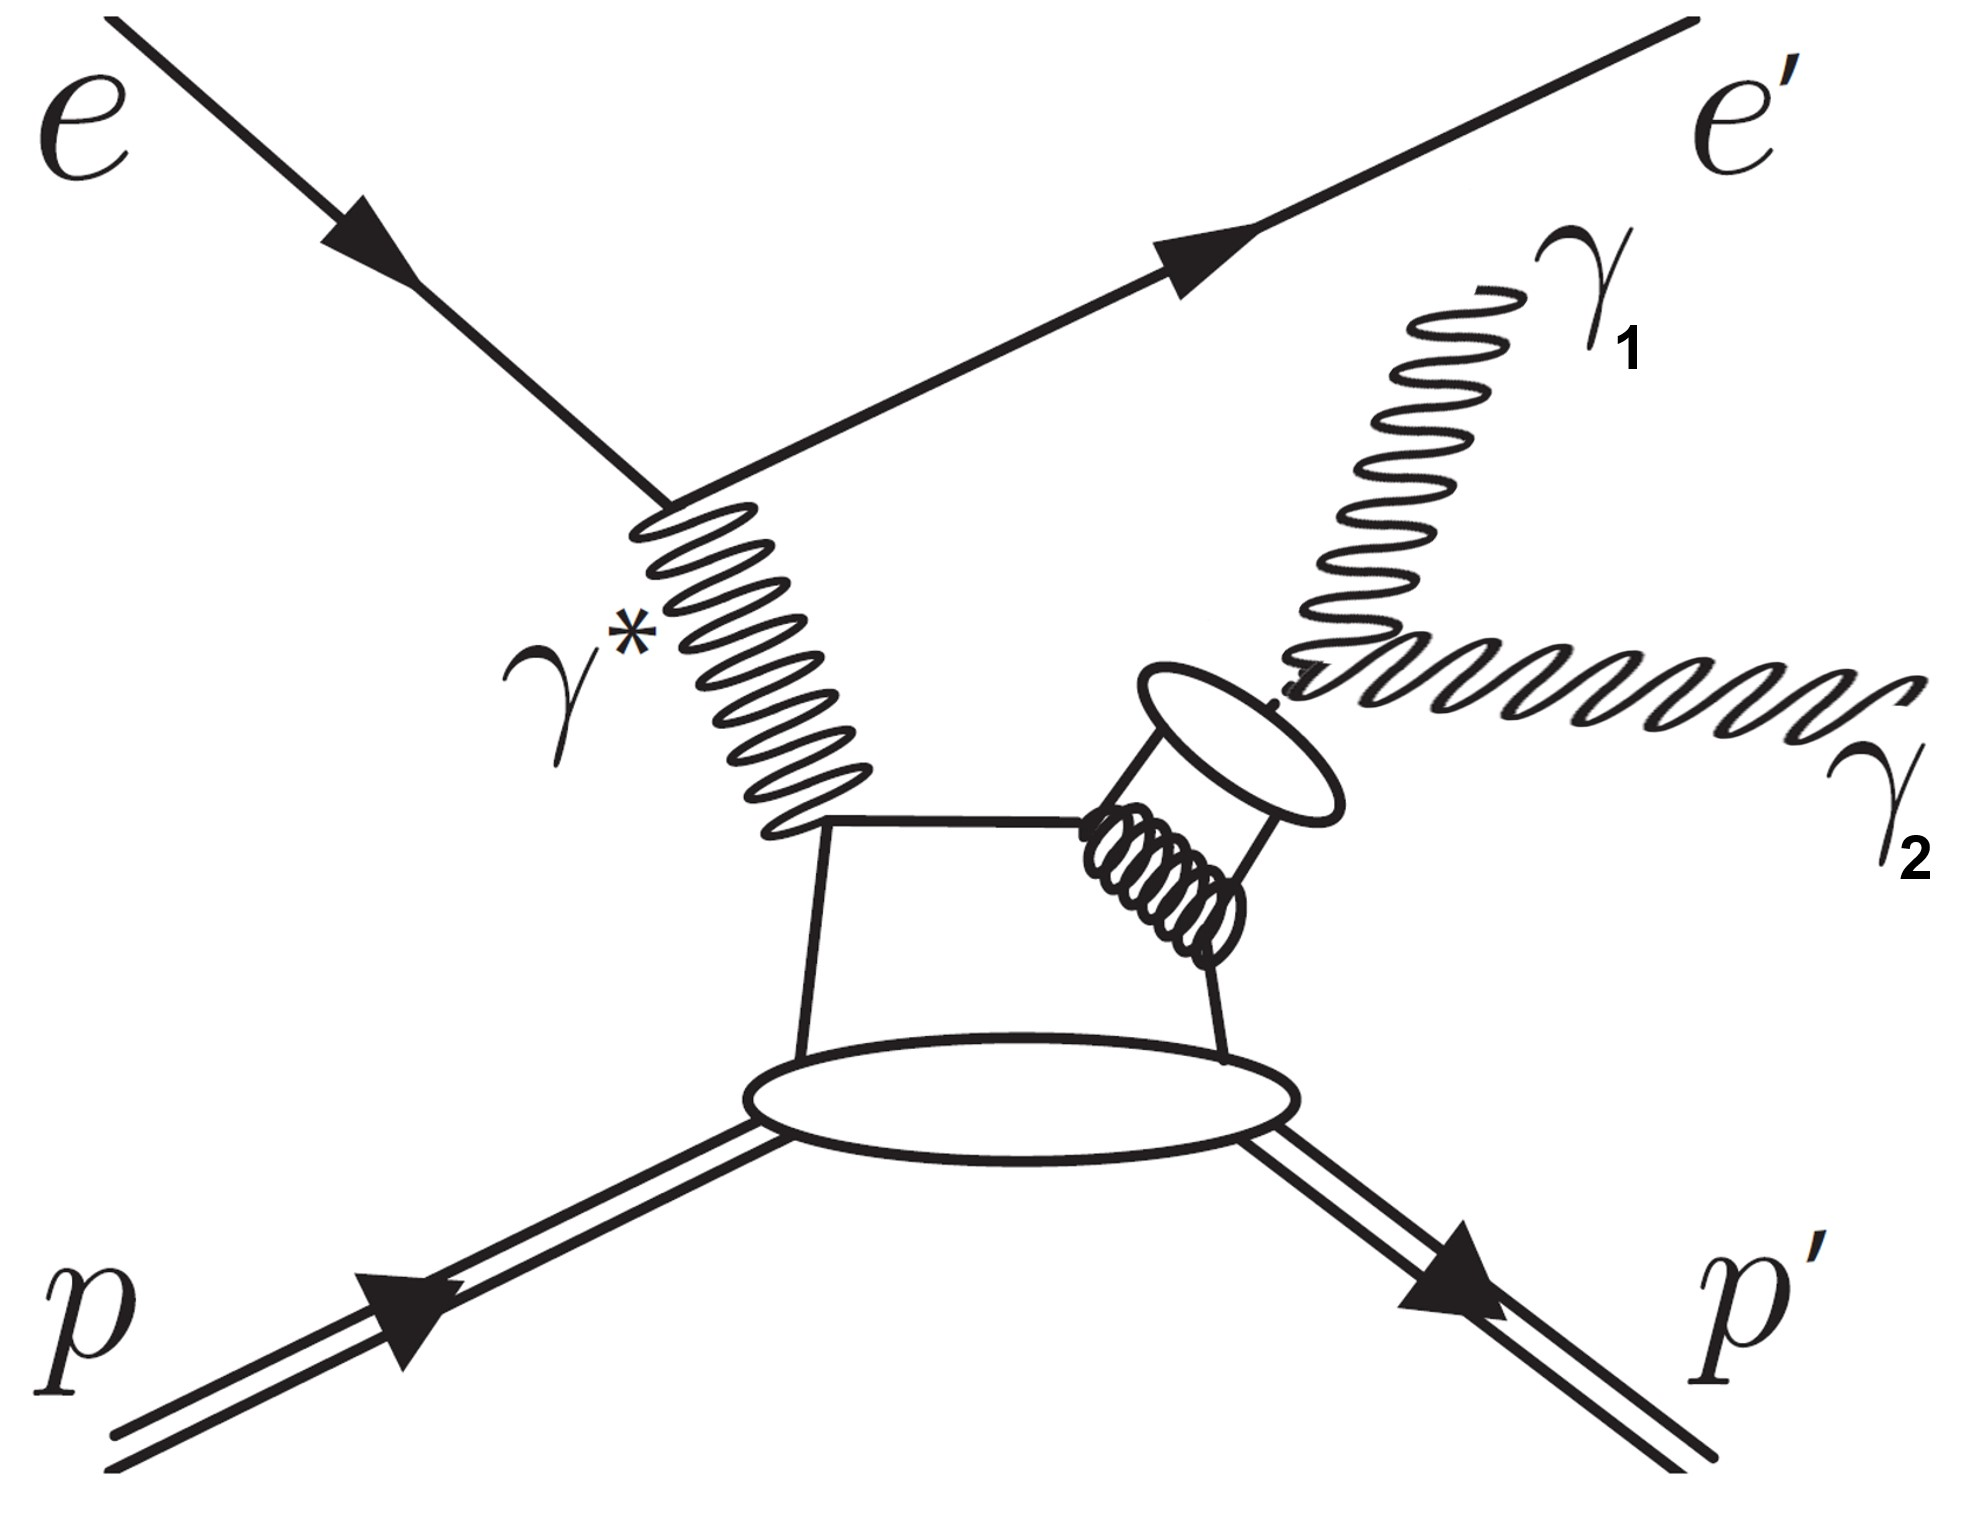
\includegraphics[trim={0 0 0 0cm} ,clip,width=.95\textwidth]{DNP/dvPiP_Feynman_diagram_2.jpg}
            
            
            
            \column{0.65\textwidth}
                \begin{itemize}
                    \setlength\itemsep{1em}
                    \item 4-fold differential cross section $\frac{d\sigma}{d\textcolor{alert}{Q^2}d\textcolor{alert}{x_B}d\textcolor{alert}{t}d\textcolor{alert}{\phi}}$ expressed in terms of:
                        \begin{itemize}
                        \setlength\itemsep{0.5em}
                            \item Virtual photon 4-momentum:  \textcolor{alert}{$Q^2$} $\equiv$  $-(p_e-p_{e'})^2$
                            \item Bjorken x: \textcolor{alert}{$x_B$} $\equiv$ $\frac{Q^2}{2p_p\cdot(p_{e}-p_{e'})}$
                            \item Momentum transfer: \textcolor{alert}{-t} $\equiv$ $-(p_{p'}-p_p)^2$
                            \item Angle between lepton \& hadron planes: \textbf{\textcolor{alert}{$\phi$}} = 
                            
                             \begin{columns}[t, onlytextwidth]
         
          \column{0.6\textwidth}
             \begin{center}
                            
                            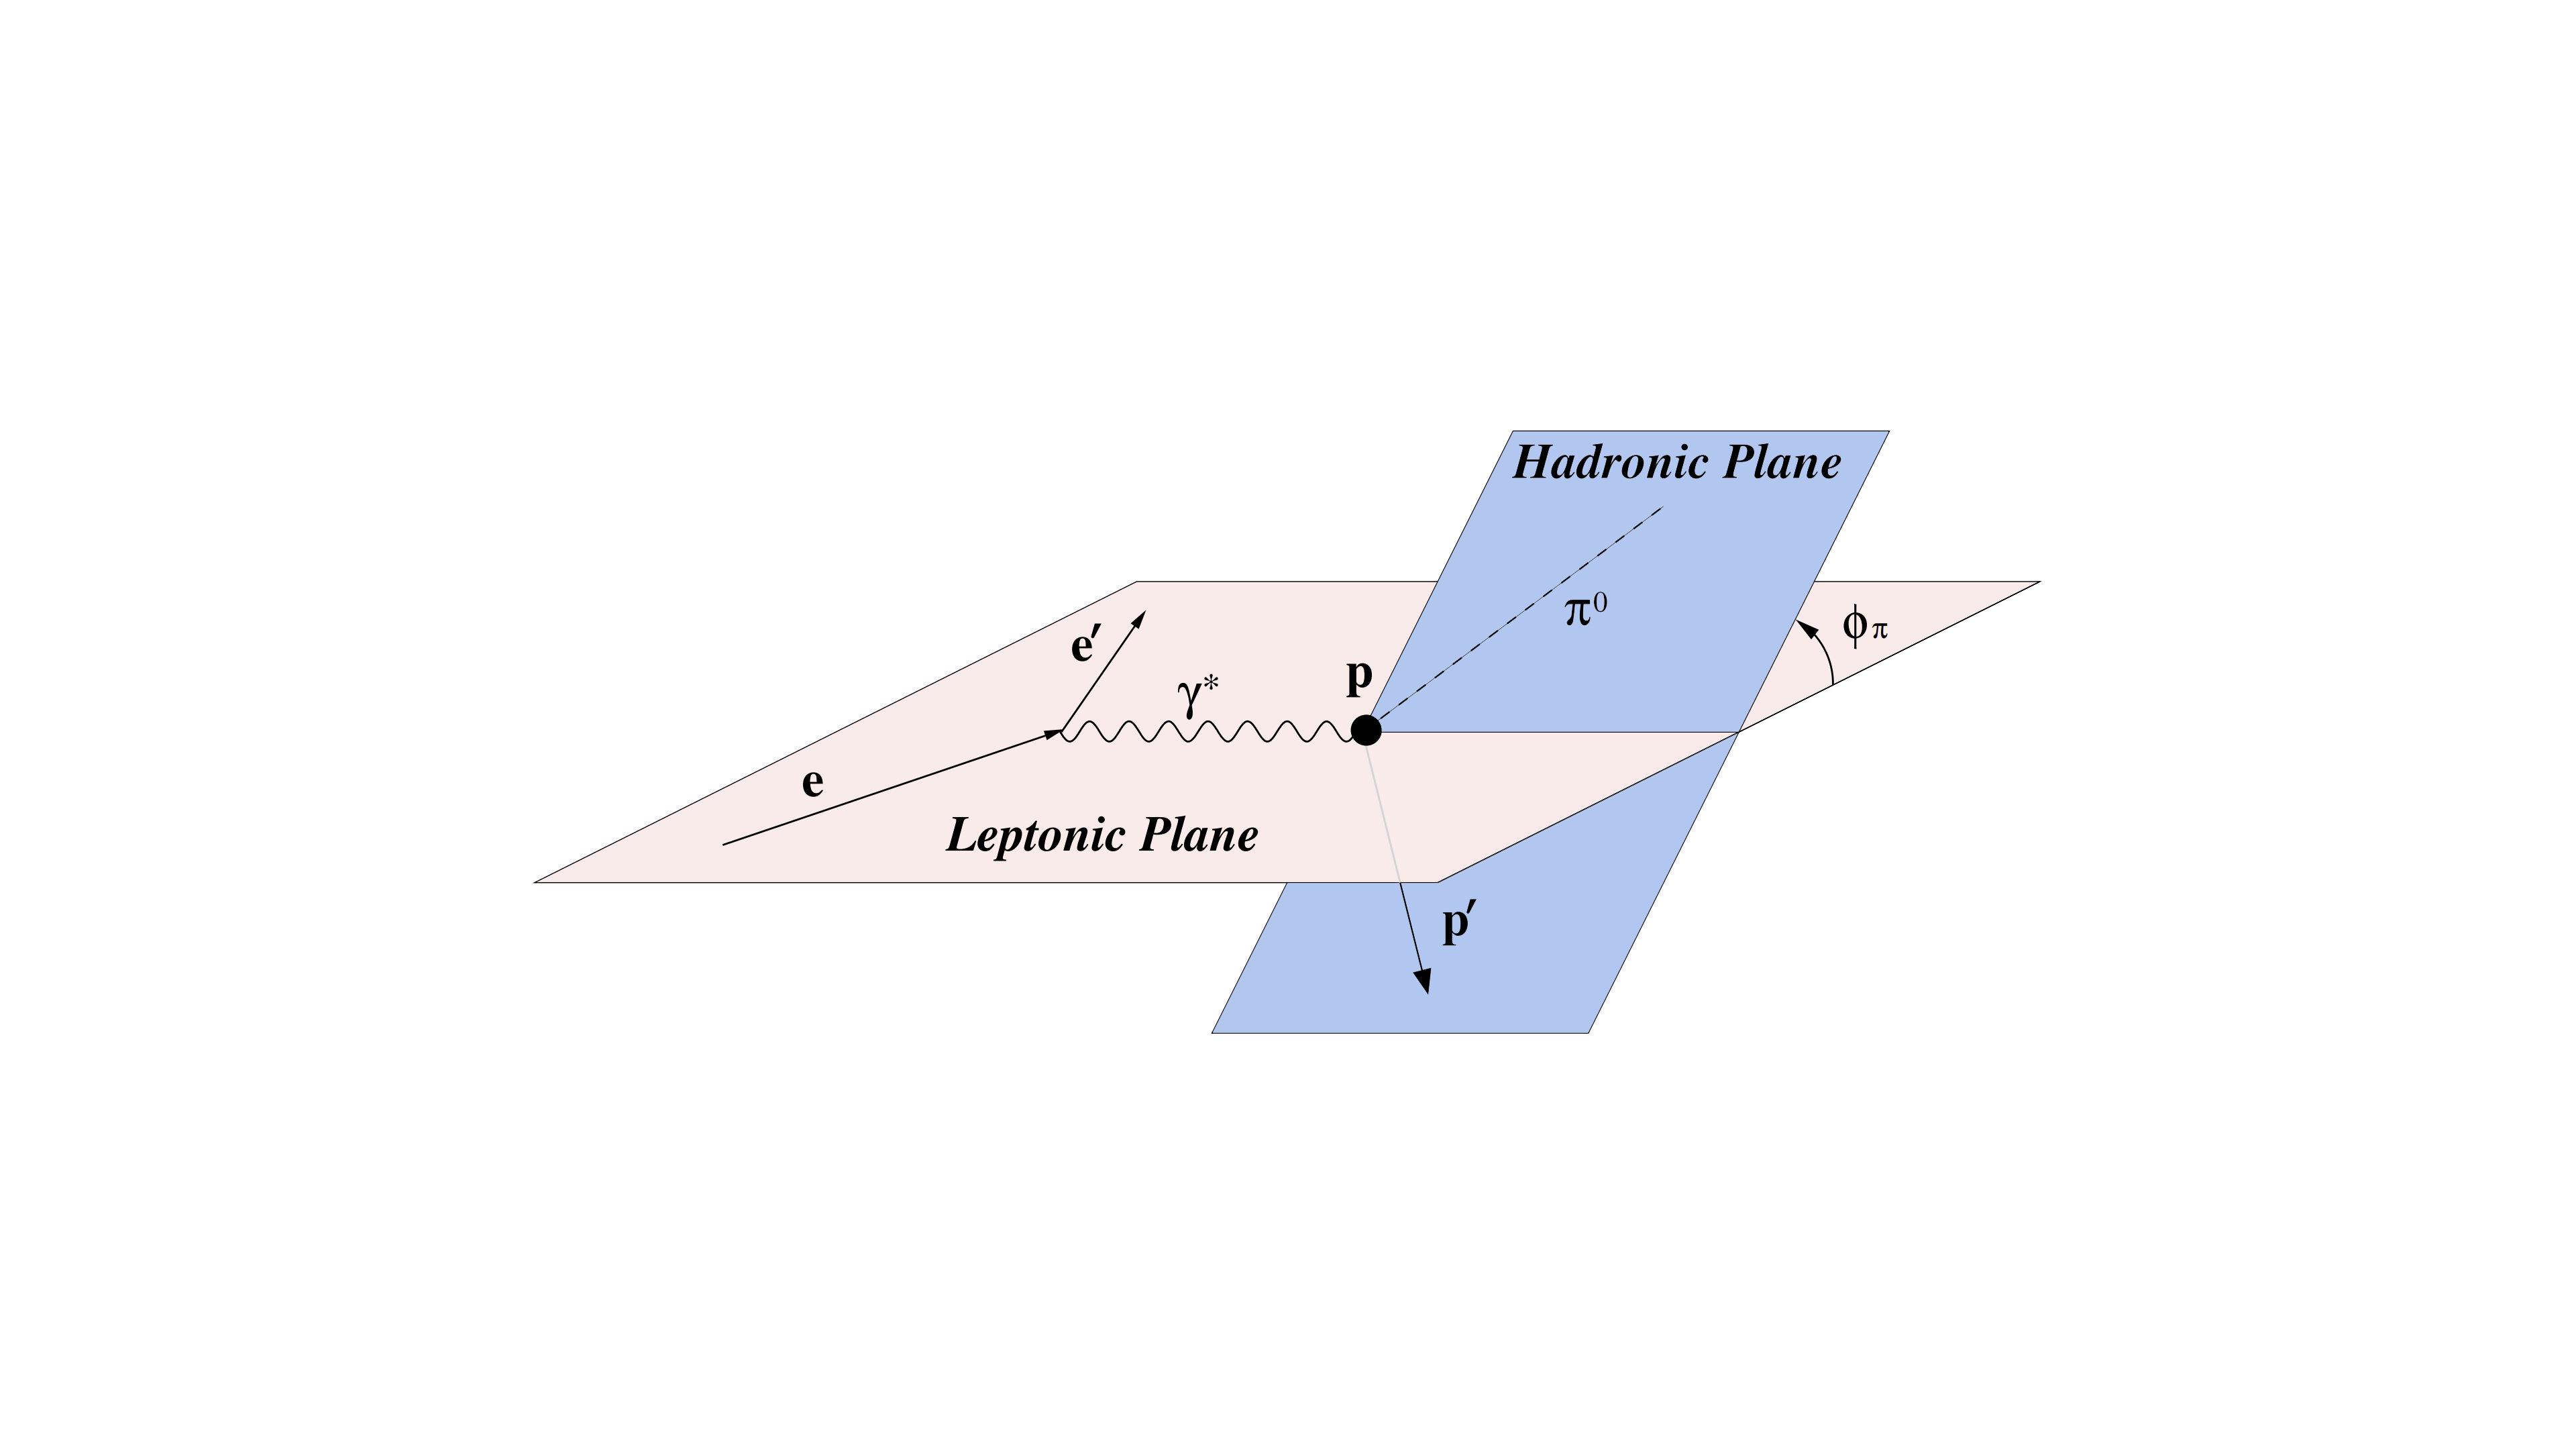
\includegraphics[trim={10cm 8cm 10cm 8cm} ,clip,width=.96546725995\textwidth]{DNP/lept_had_planes.png}
                            \end{center}
            \column{0.4\textwidth}
            \footnotesize{$\cos^{-1} \left( \frac{ \left(p_{e} \times p_{e'} \right) \cdot \left( p_{p'} \times p_{\gamma^*} \right) }{ \lVert p_{e} \times p_{e'} \rVert \: \lVert p_{p'} \times p_{\gamma^*} \rVert} \right)$}
          
          \vspace{1.5cm}
          {\myfont{\tiny     \textcolor{white}{lllllll} Images from S. Lee, A. Kim   }}
         \end{columns}
                            
                        \end{itemize}
                                            
                    \item In DIS regime: W$>2$GeV, $Q^2$> 1GeV$^2$
                \end{itemize}
                
     
                               
        \end{columns}
\end{frame}    







    

    
\begin{frame}{\textbf{Analysis Goal}: Extract DV$\pi^o$P Cross Section}
    Extracting the cross section for the process will extend the CLAS6 work to a larger kinematic range with higher statistics
        \begin{columns}
            \column{0.5\textwidth}
            \begin{figure}[H]
            \centering
            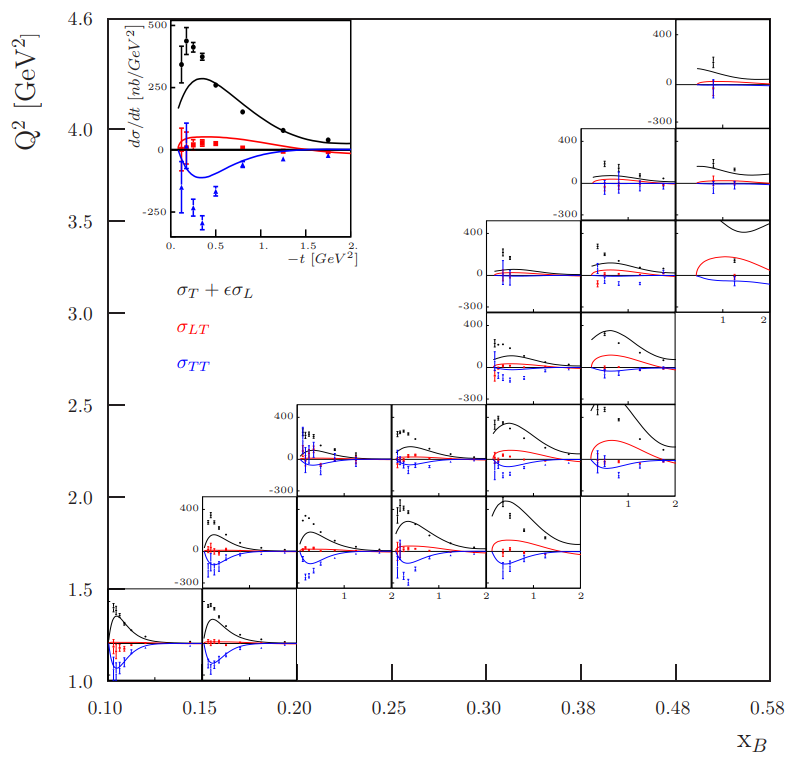
\includegraphics[width=.8\textwidth]{Pics/Goal/clas6CrossSection.png}
            \label{fig:clas6}
            \end{figure}
            
             \column{0.5\textwidth}
             \centering$Q^2$ vs. $x_B$ - CLAS12
             %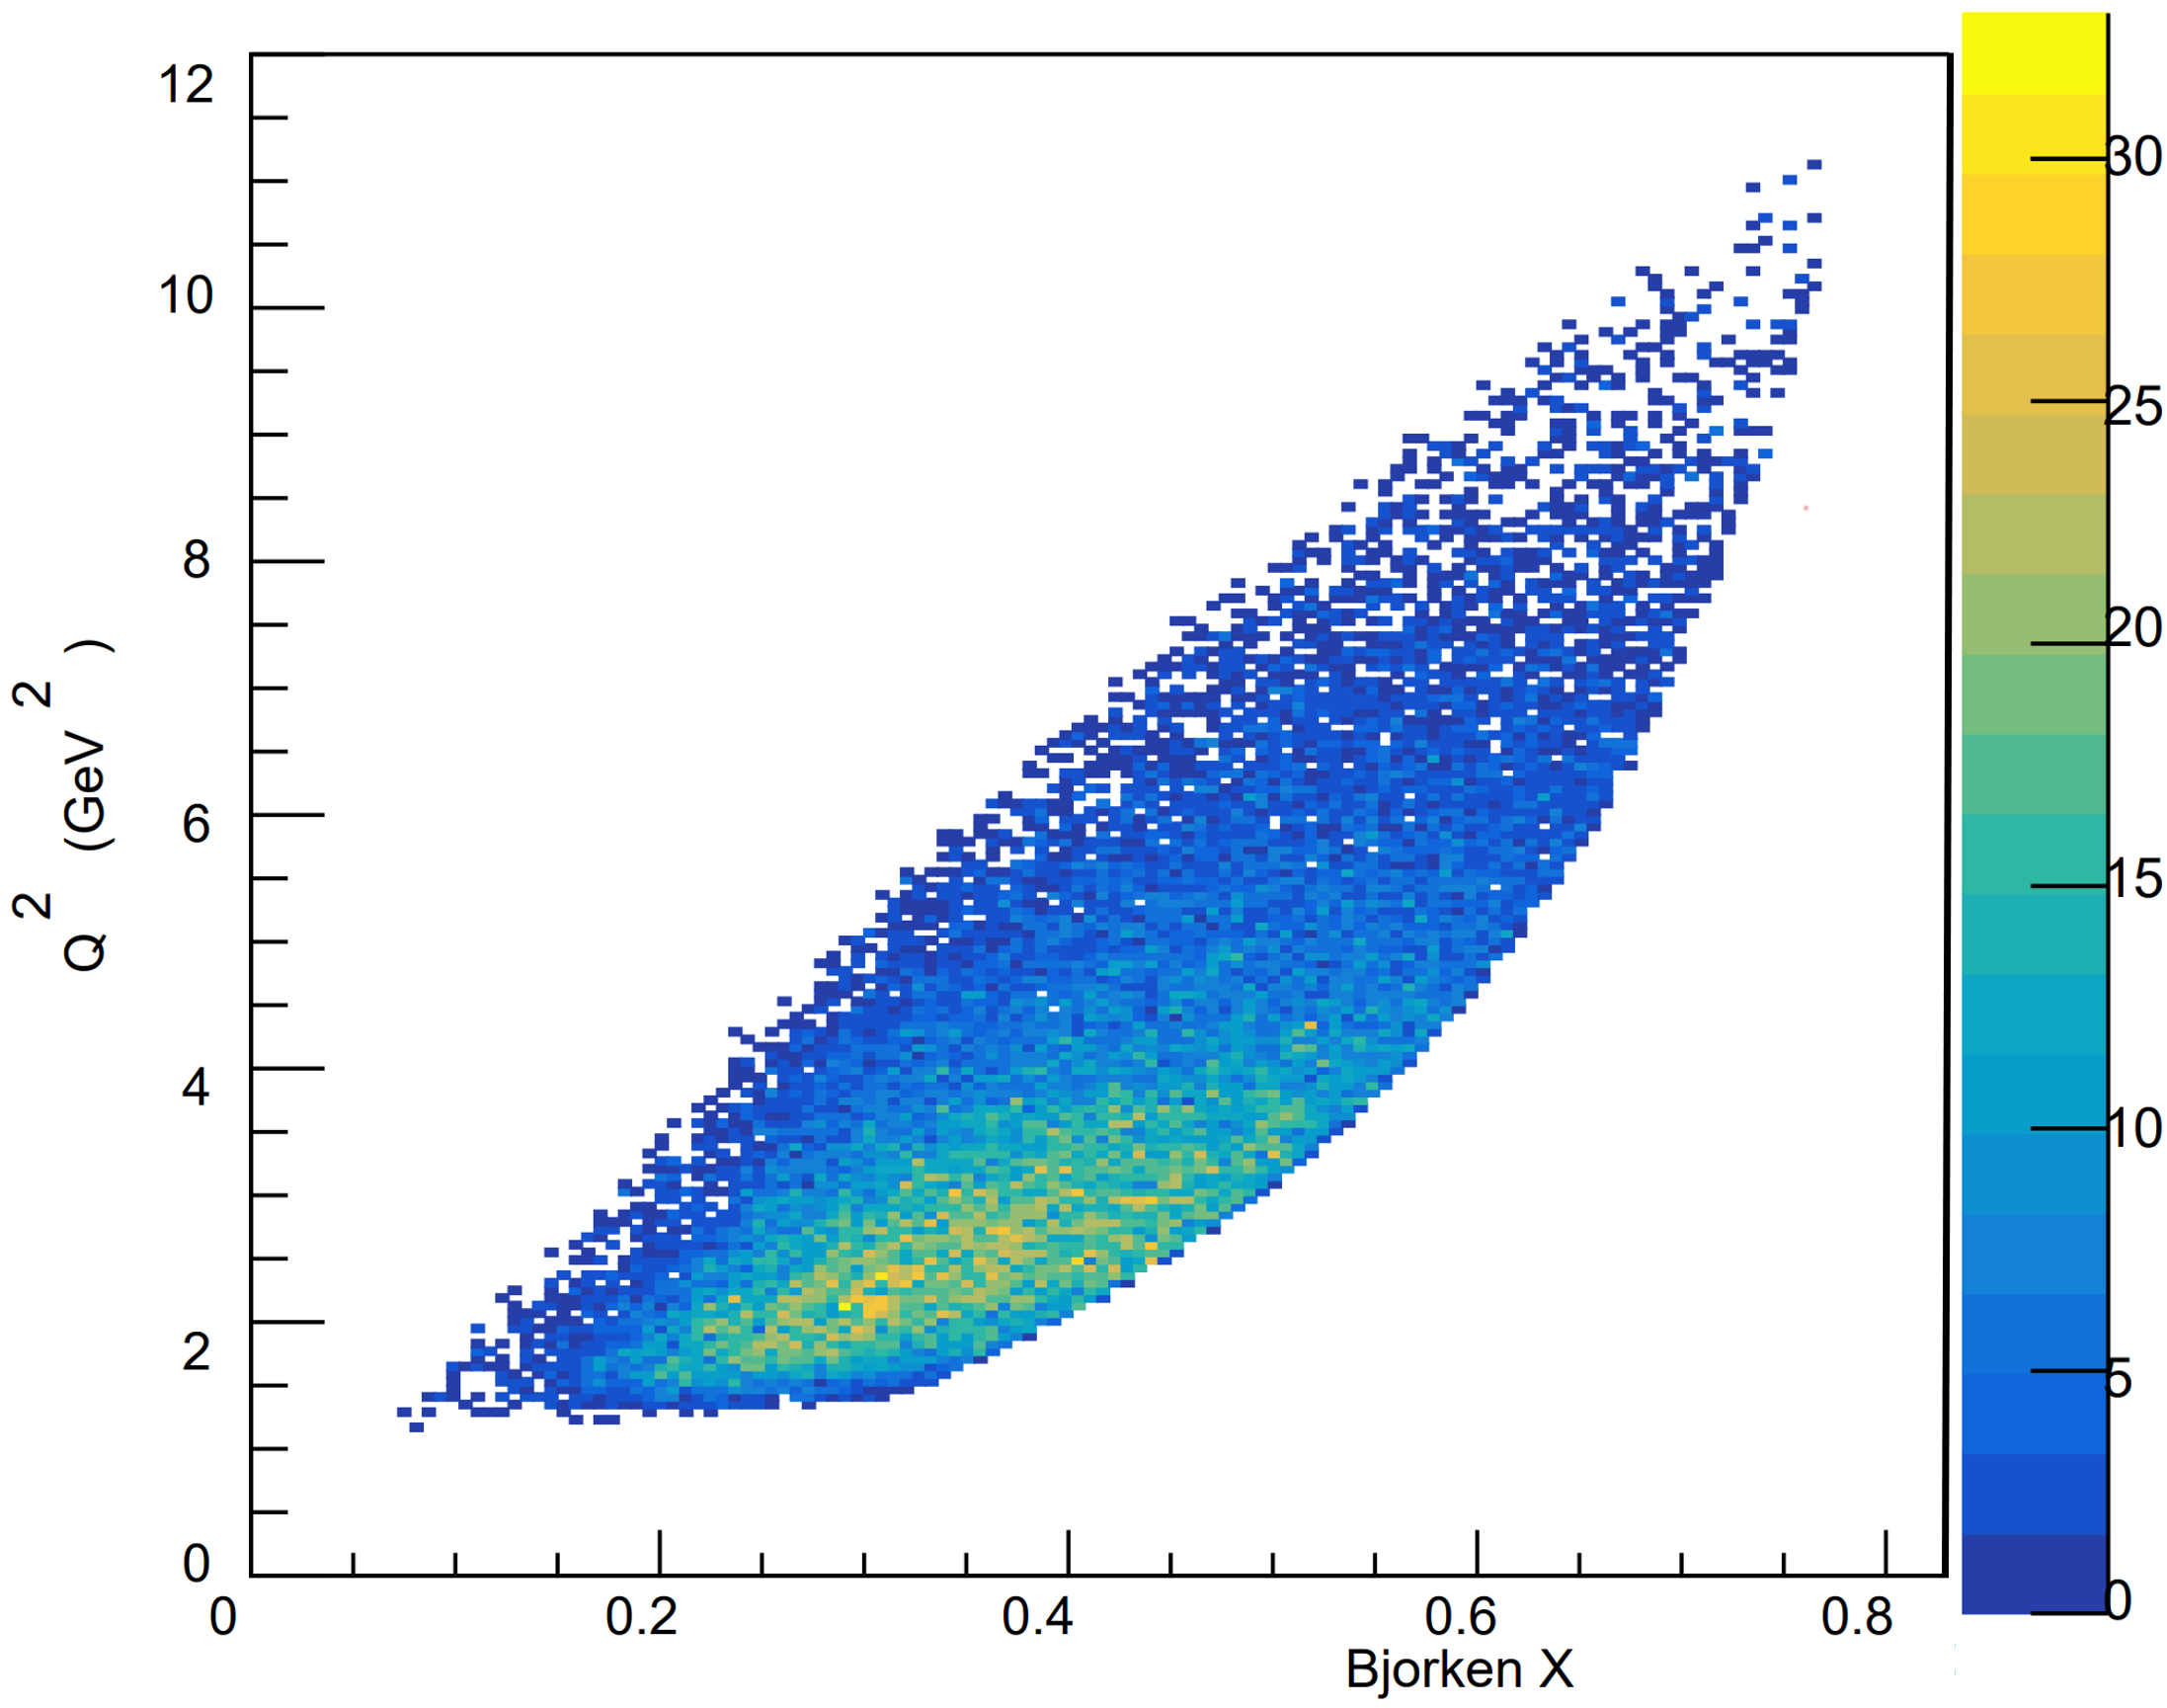
\includegraphics[width=.9\textwidth]{Pics/kinreach/bjorken_x_cropped.png}
             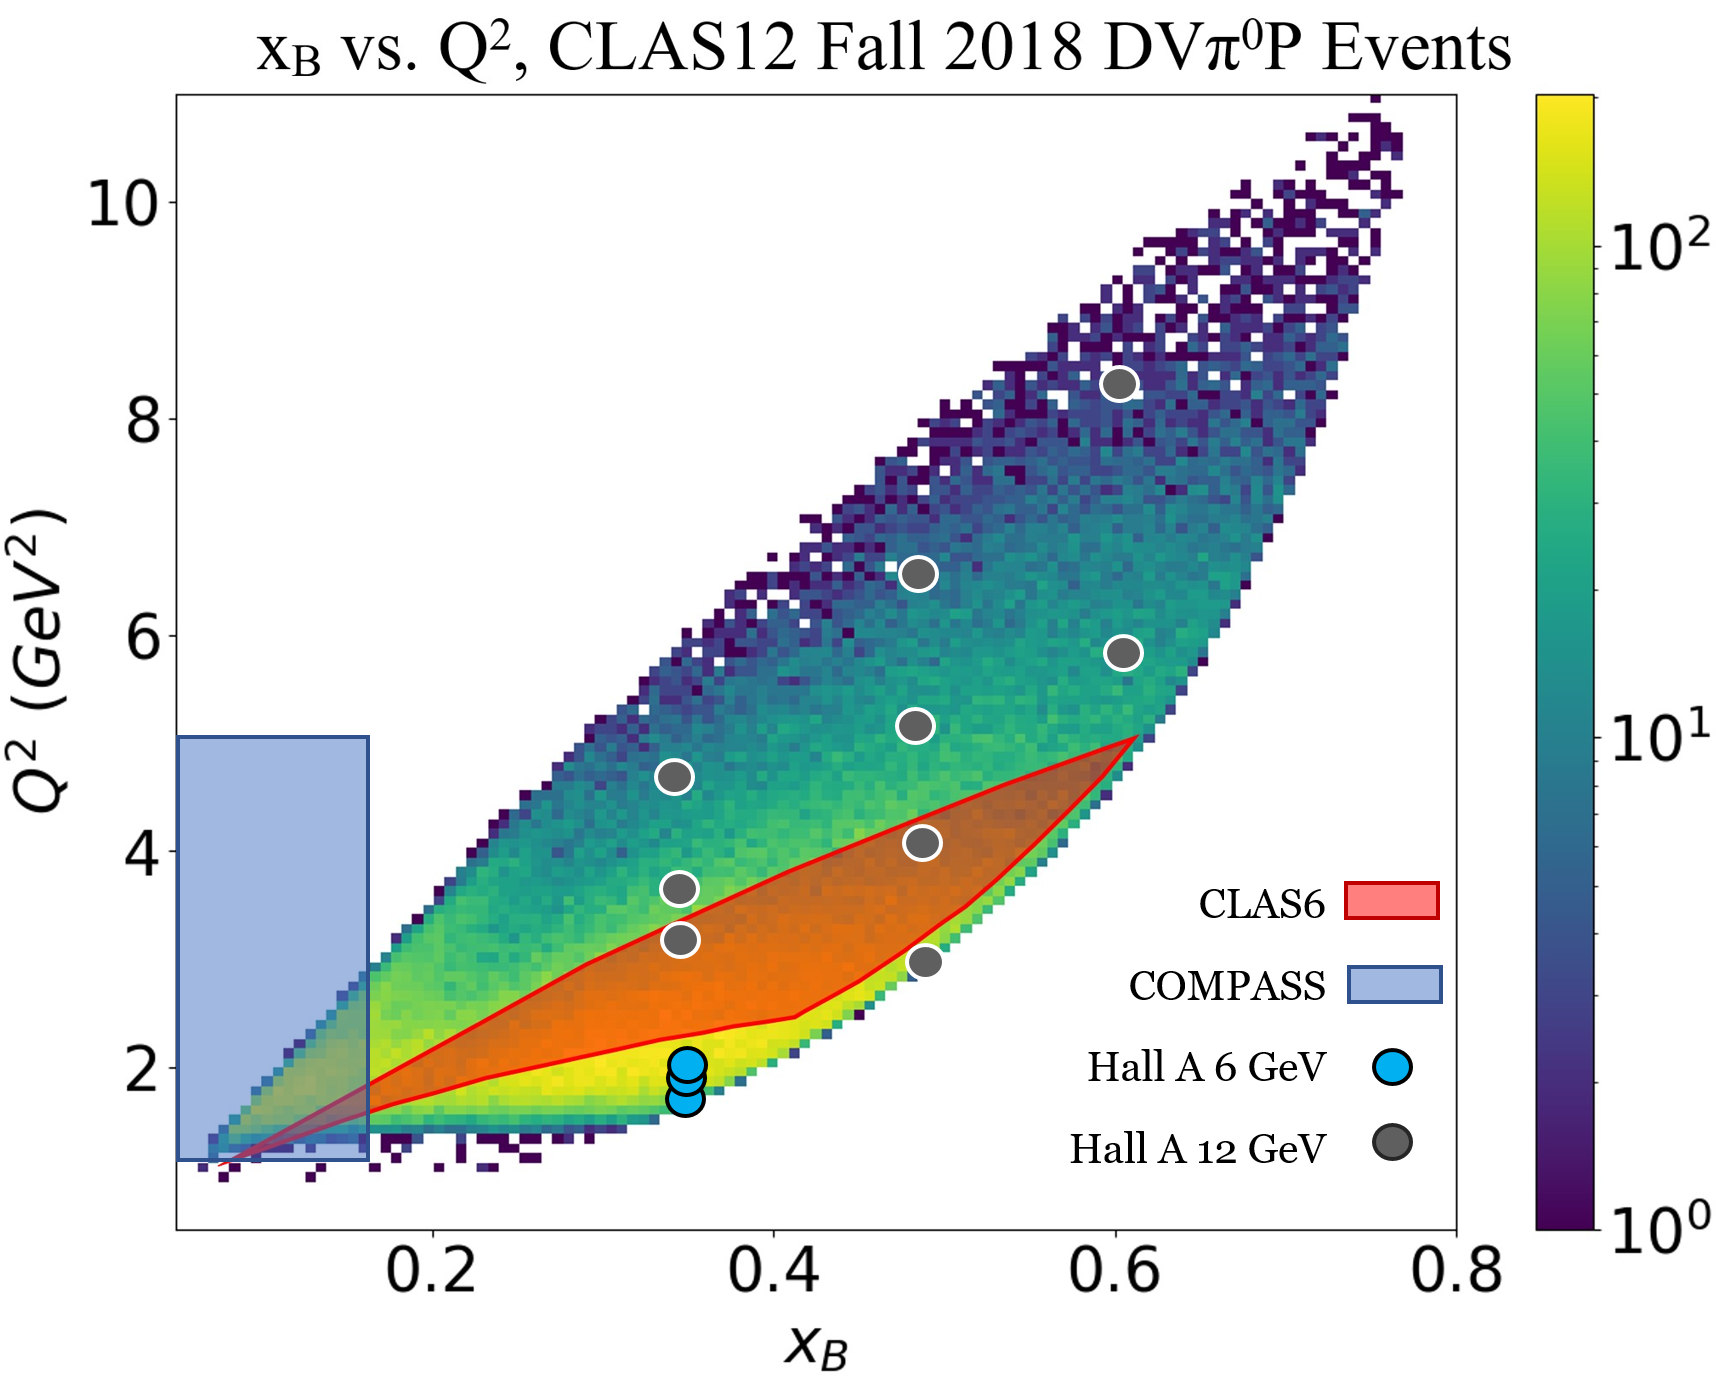
\includegraphics[trim={0 0 0 1.8cm} ,clip,width=.9725995\textwidth]{APS_2022/clas12_vs_clas6_kinematic_coverage.png}
    \end{columns}
    
    {\myfont{\tiny     [I. Bedlinskiy et al., PRC, 90, 025205     (2014)]   }}

\end{frame}


\begin{frame}{The Path to Measurement has Many Steps}
        \begin{columns}[t, onlytextwidth]
            \column{0.45\textwidth}
            
            \begin{itemize}
                \item \textbf{Design and Build Detectors}: 2006-2018
                \item \textbf{Take Data}: 2018 start, continuing
                \item \textbf{Process Data}: Reconstruct particle paths from detector signals 
                \item \textbf{Analyze Data}: Event selection to find raw process rates
                \item \textbf{Correct Data}: Run simulations and apply correction factors
                \item \textbf{Extract Physics}: Calculate structure functions, deconvolve GPDS, 
            \end{itemize}
            \column{0.6\textwidth}
                    \begin{figure}
                        \centering
                        \includegraphics[trim={0 0 0 0} ,clip,width=.8579562\textwidth]{Introduction/wirestring.png}
                        
                        %\caption{Parton Distribution Function at $Q^2=10GeV^2$}
                        %\caption{                       {\myfont{\tiny  [Quanta Magazine 20190911]   }}}
                        %Source  https://home.cern/science/engineering/accelerating-radiofrequency-cavities
                         
                    \end{figure} 
    \centering
                        Detector construction - wire chamber stringing\\
                         {\myfont{\tiny[V. Burkert et al., NIMA, 959, 163419 (2020)] }}
                    %\begin{figure}
                    %    \centering
                    %    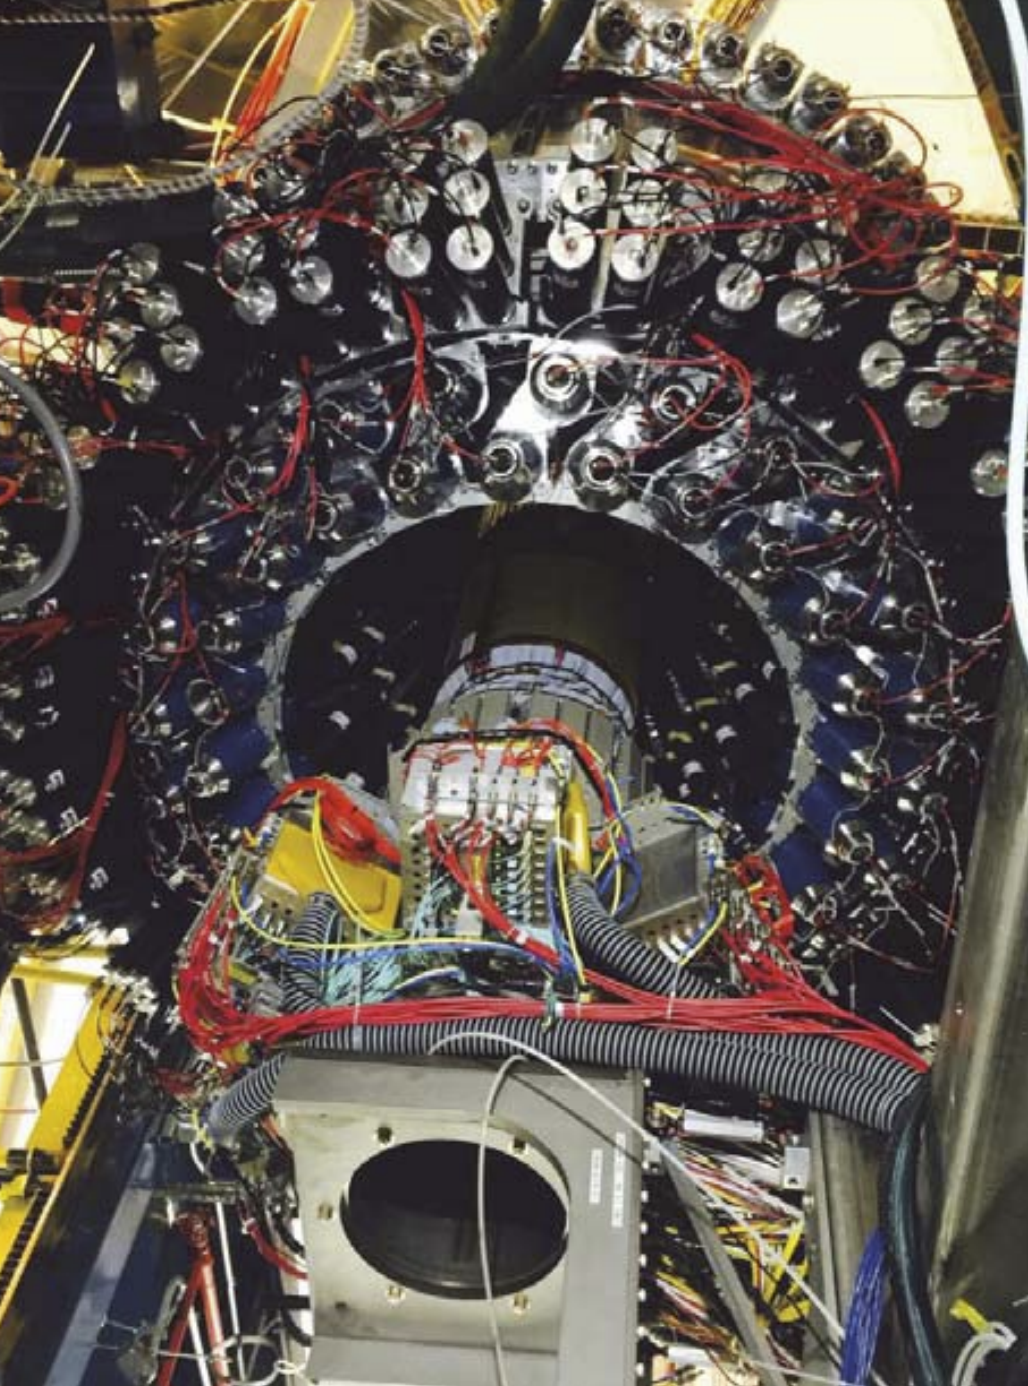
\includegraphics[angle=90,trim={0 0 0 0} ,clip,width=.579562\textwidth]{Introduction/Centraldet.png}
                    %    \caption{Detector Construction [V. Burkert et al., NIMA, 959, 163419 (2020)] }
                    %    \label{fig:awesome_image}
                    %\end{figure}
                 
        \end{columns}
        

\end{frame}


\begin{frame}{Jefferson Lab 10.6 GeV CEBAF Accelerator} \label{frame:datasets1}
        Thomas Jefferson National Accelerator Facility - Newport News, VA
        
        \begin{columns}[t, onlytextwidth]
            \column{0.5\textwidth}
                %\vspace{1cm}
                \begin{figure}[t!]
                    %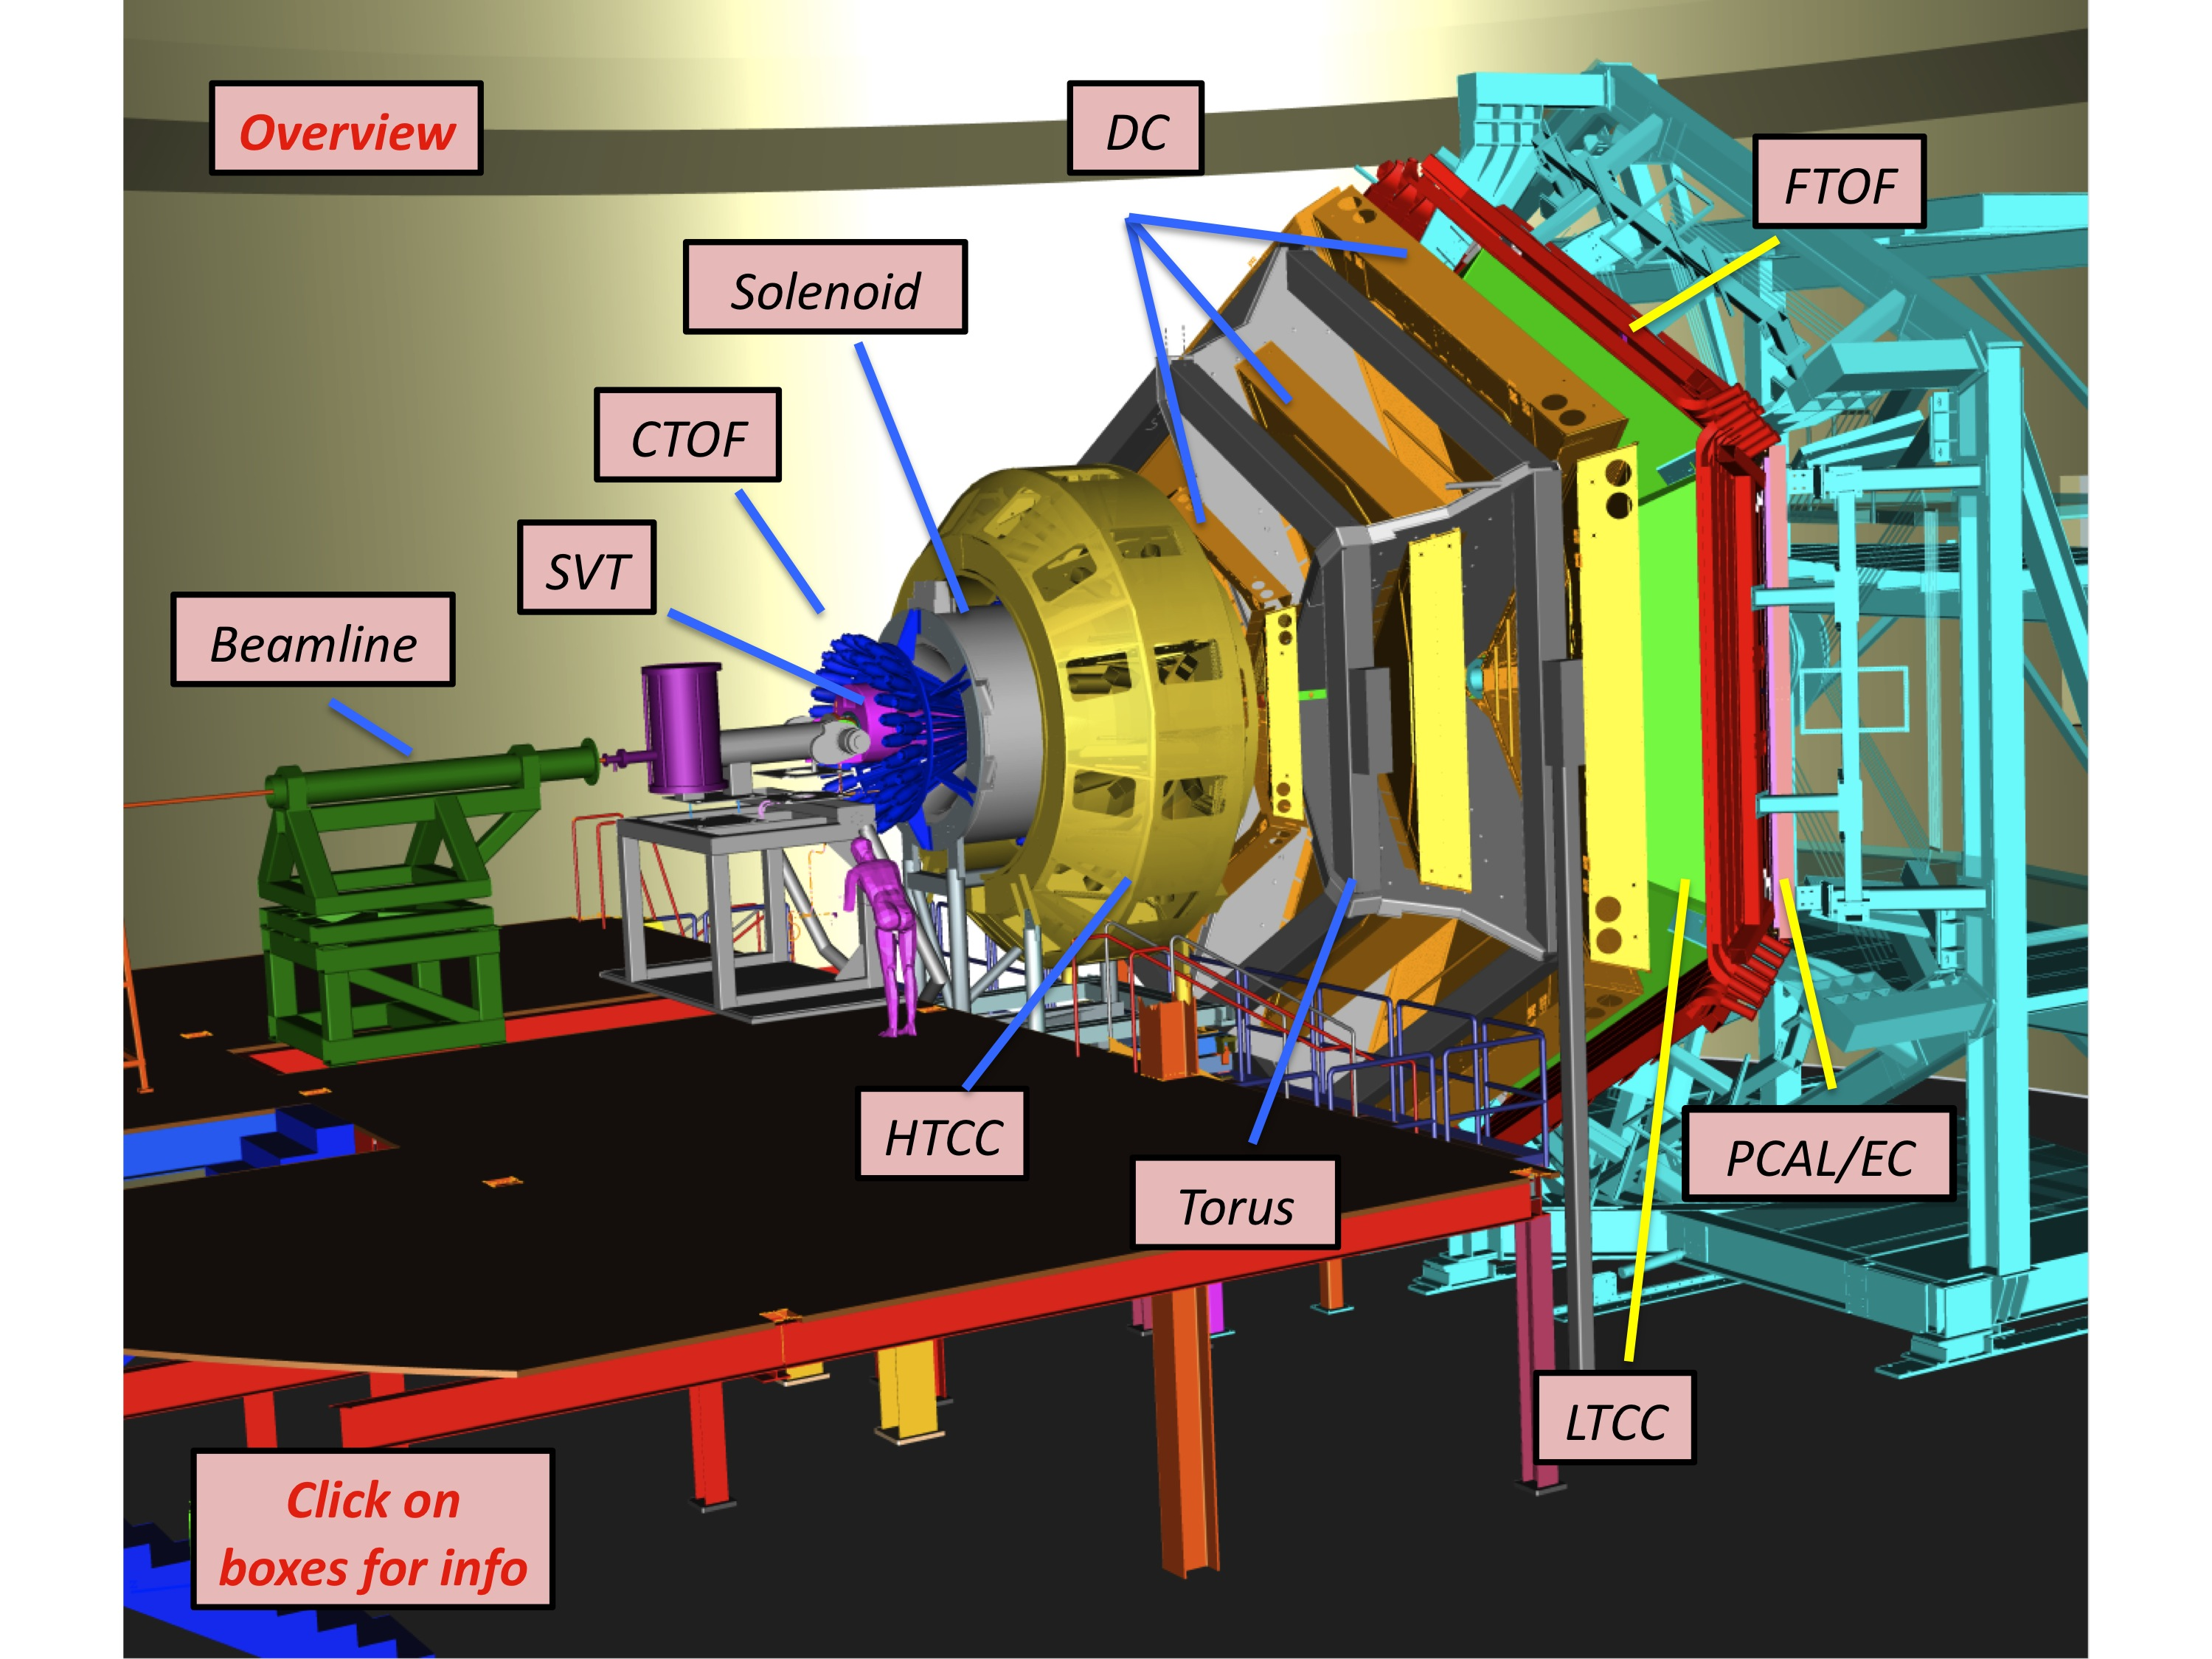
\includegraphics[height=\dimexpr0.5\textheight-0.5in]{Pics/dnp/clas12-overview.jpg}
                    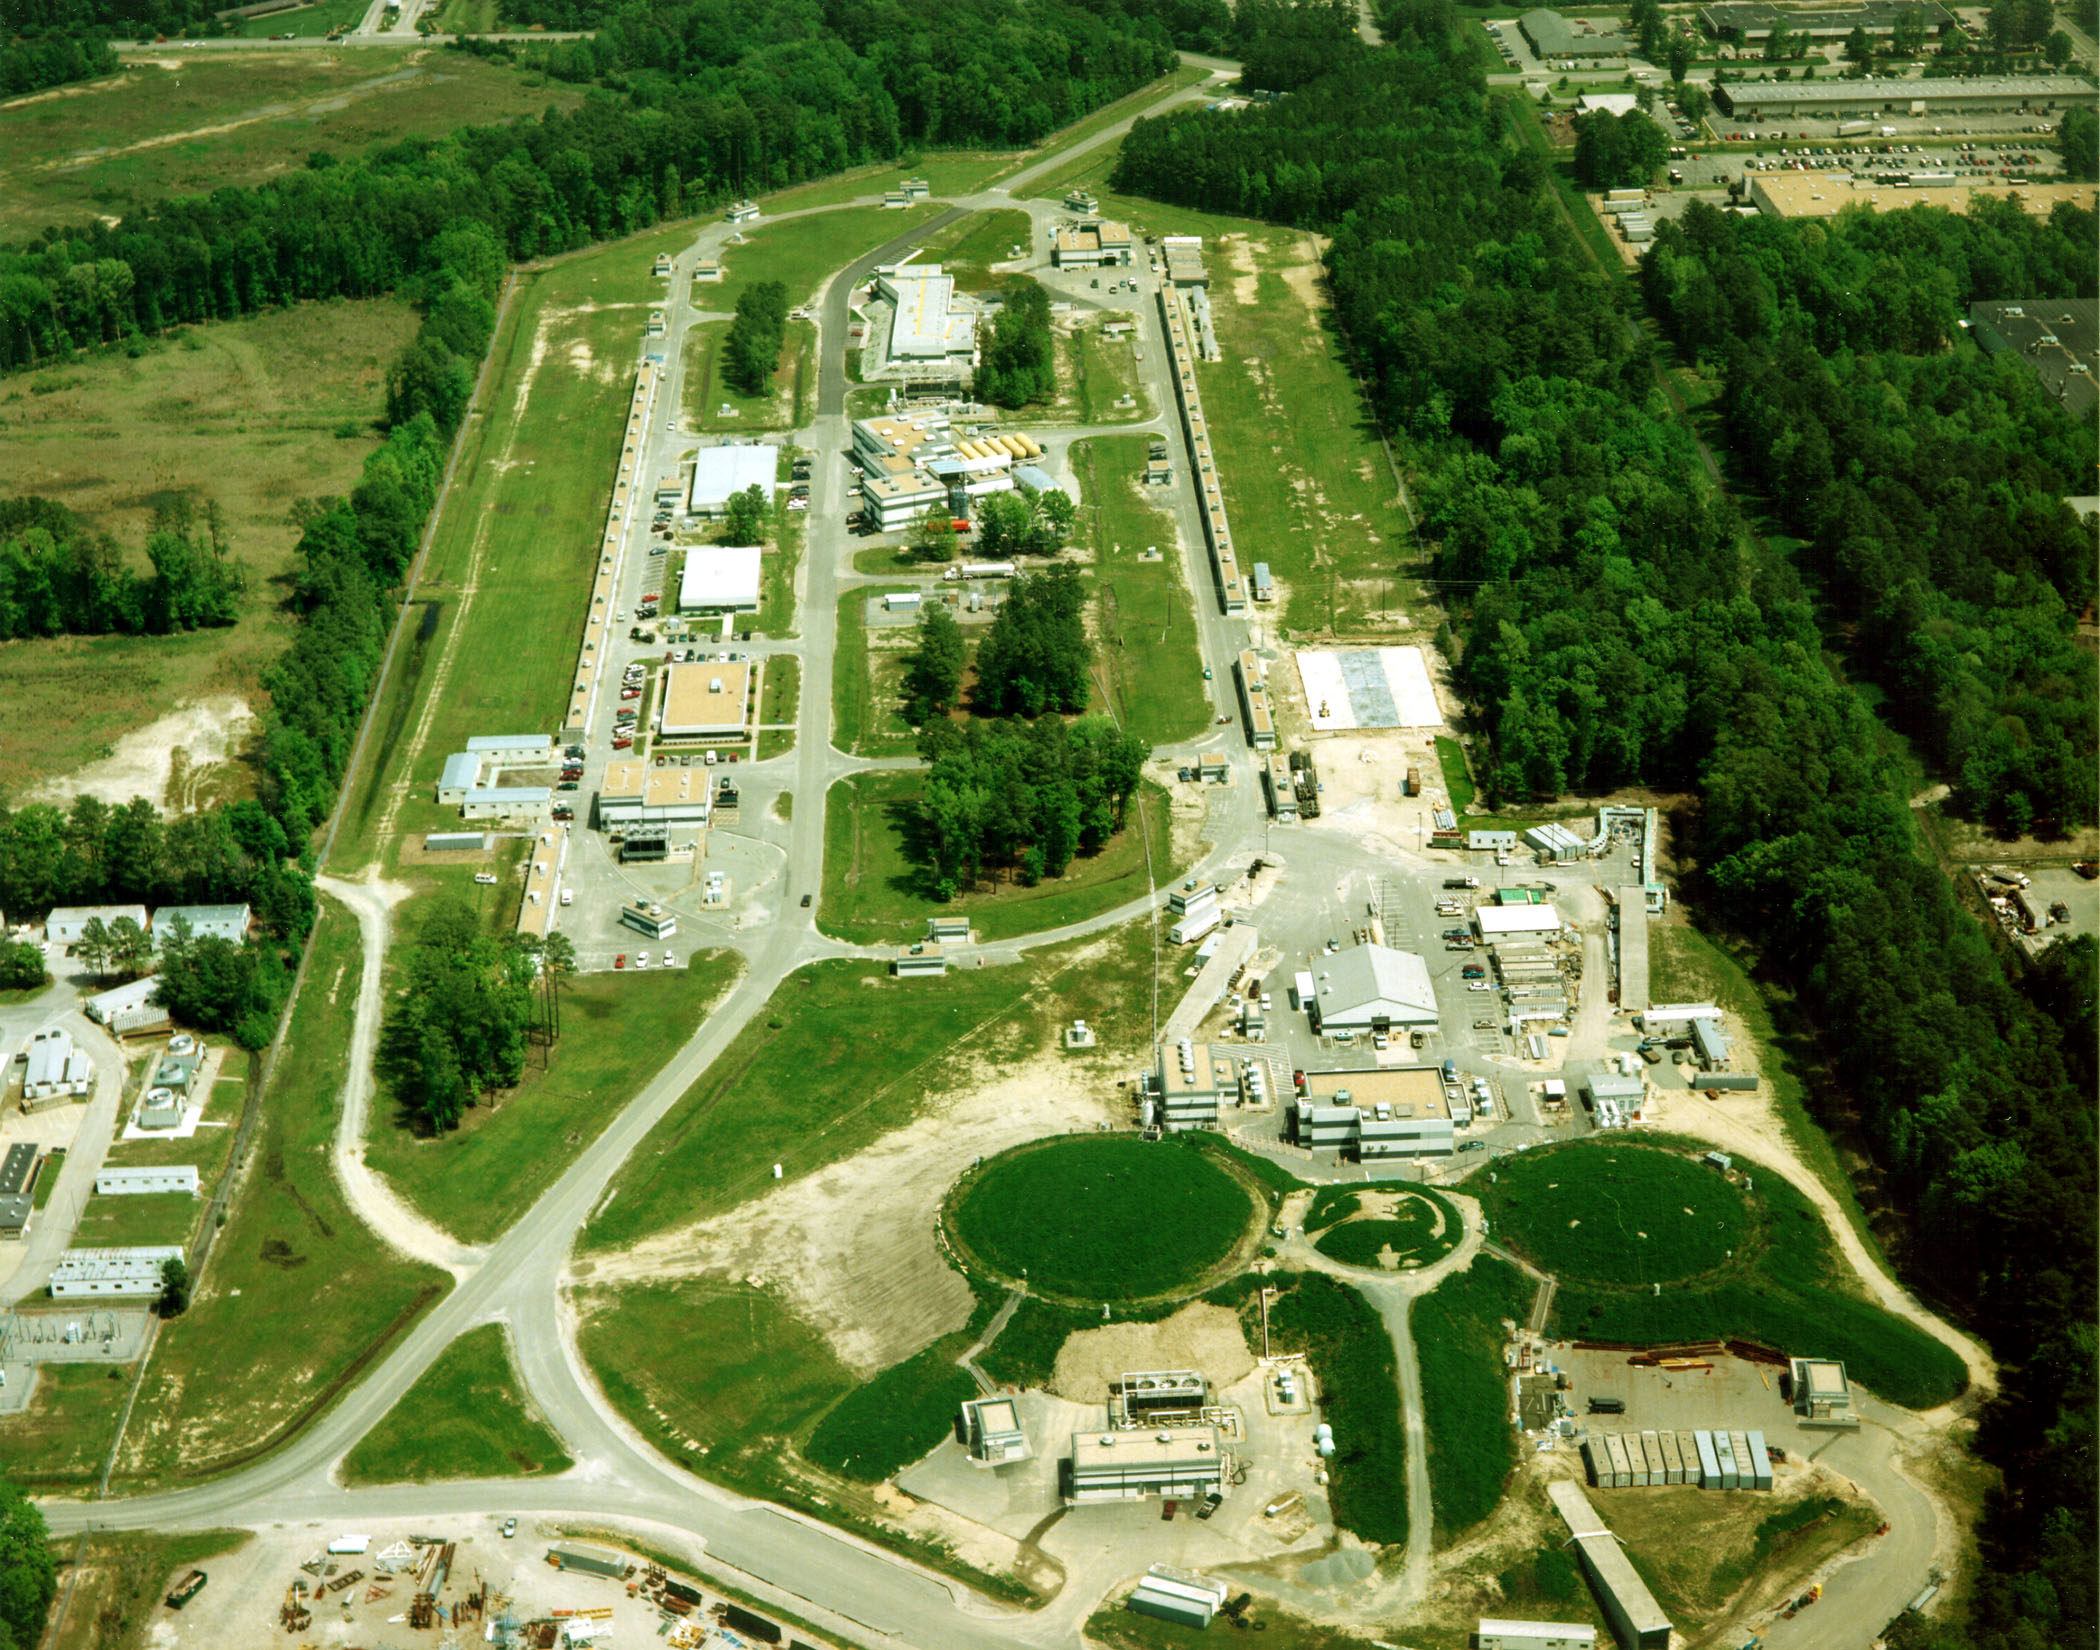
\includegraphics[width=.76349\textwidth]{Introduction/jlab.jpg}
                    
                    
                \end{figure}
                \vspace{-0.45cm}
            \begin{itemize}
                    \setlength\itemsep{1em}
                    \item Jefferson Lab aerial view
                    {\myfont{\tiny [jlab.org] }}
                    \end{itemize}
                    
            \column{0.5\textwidth}
                \begin{figure}[t!]
                    %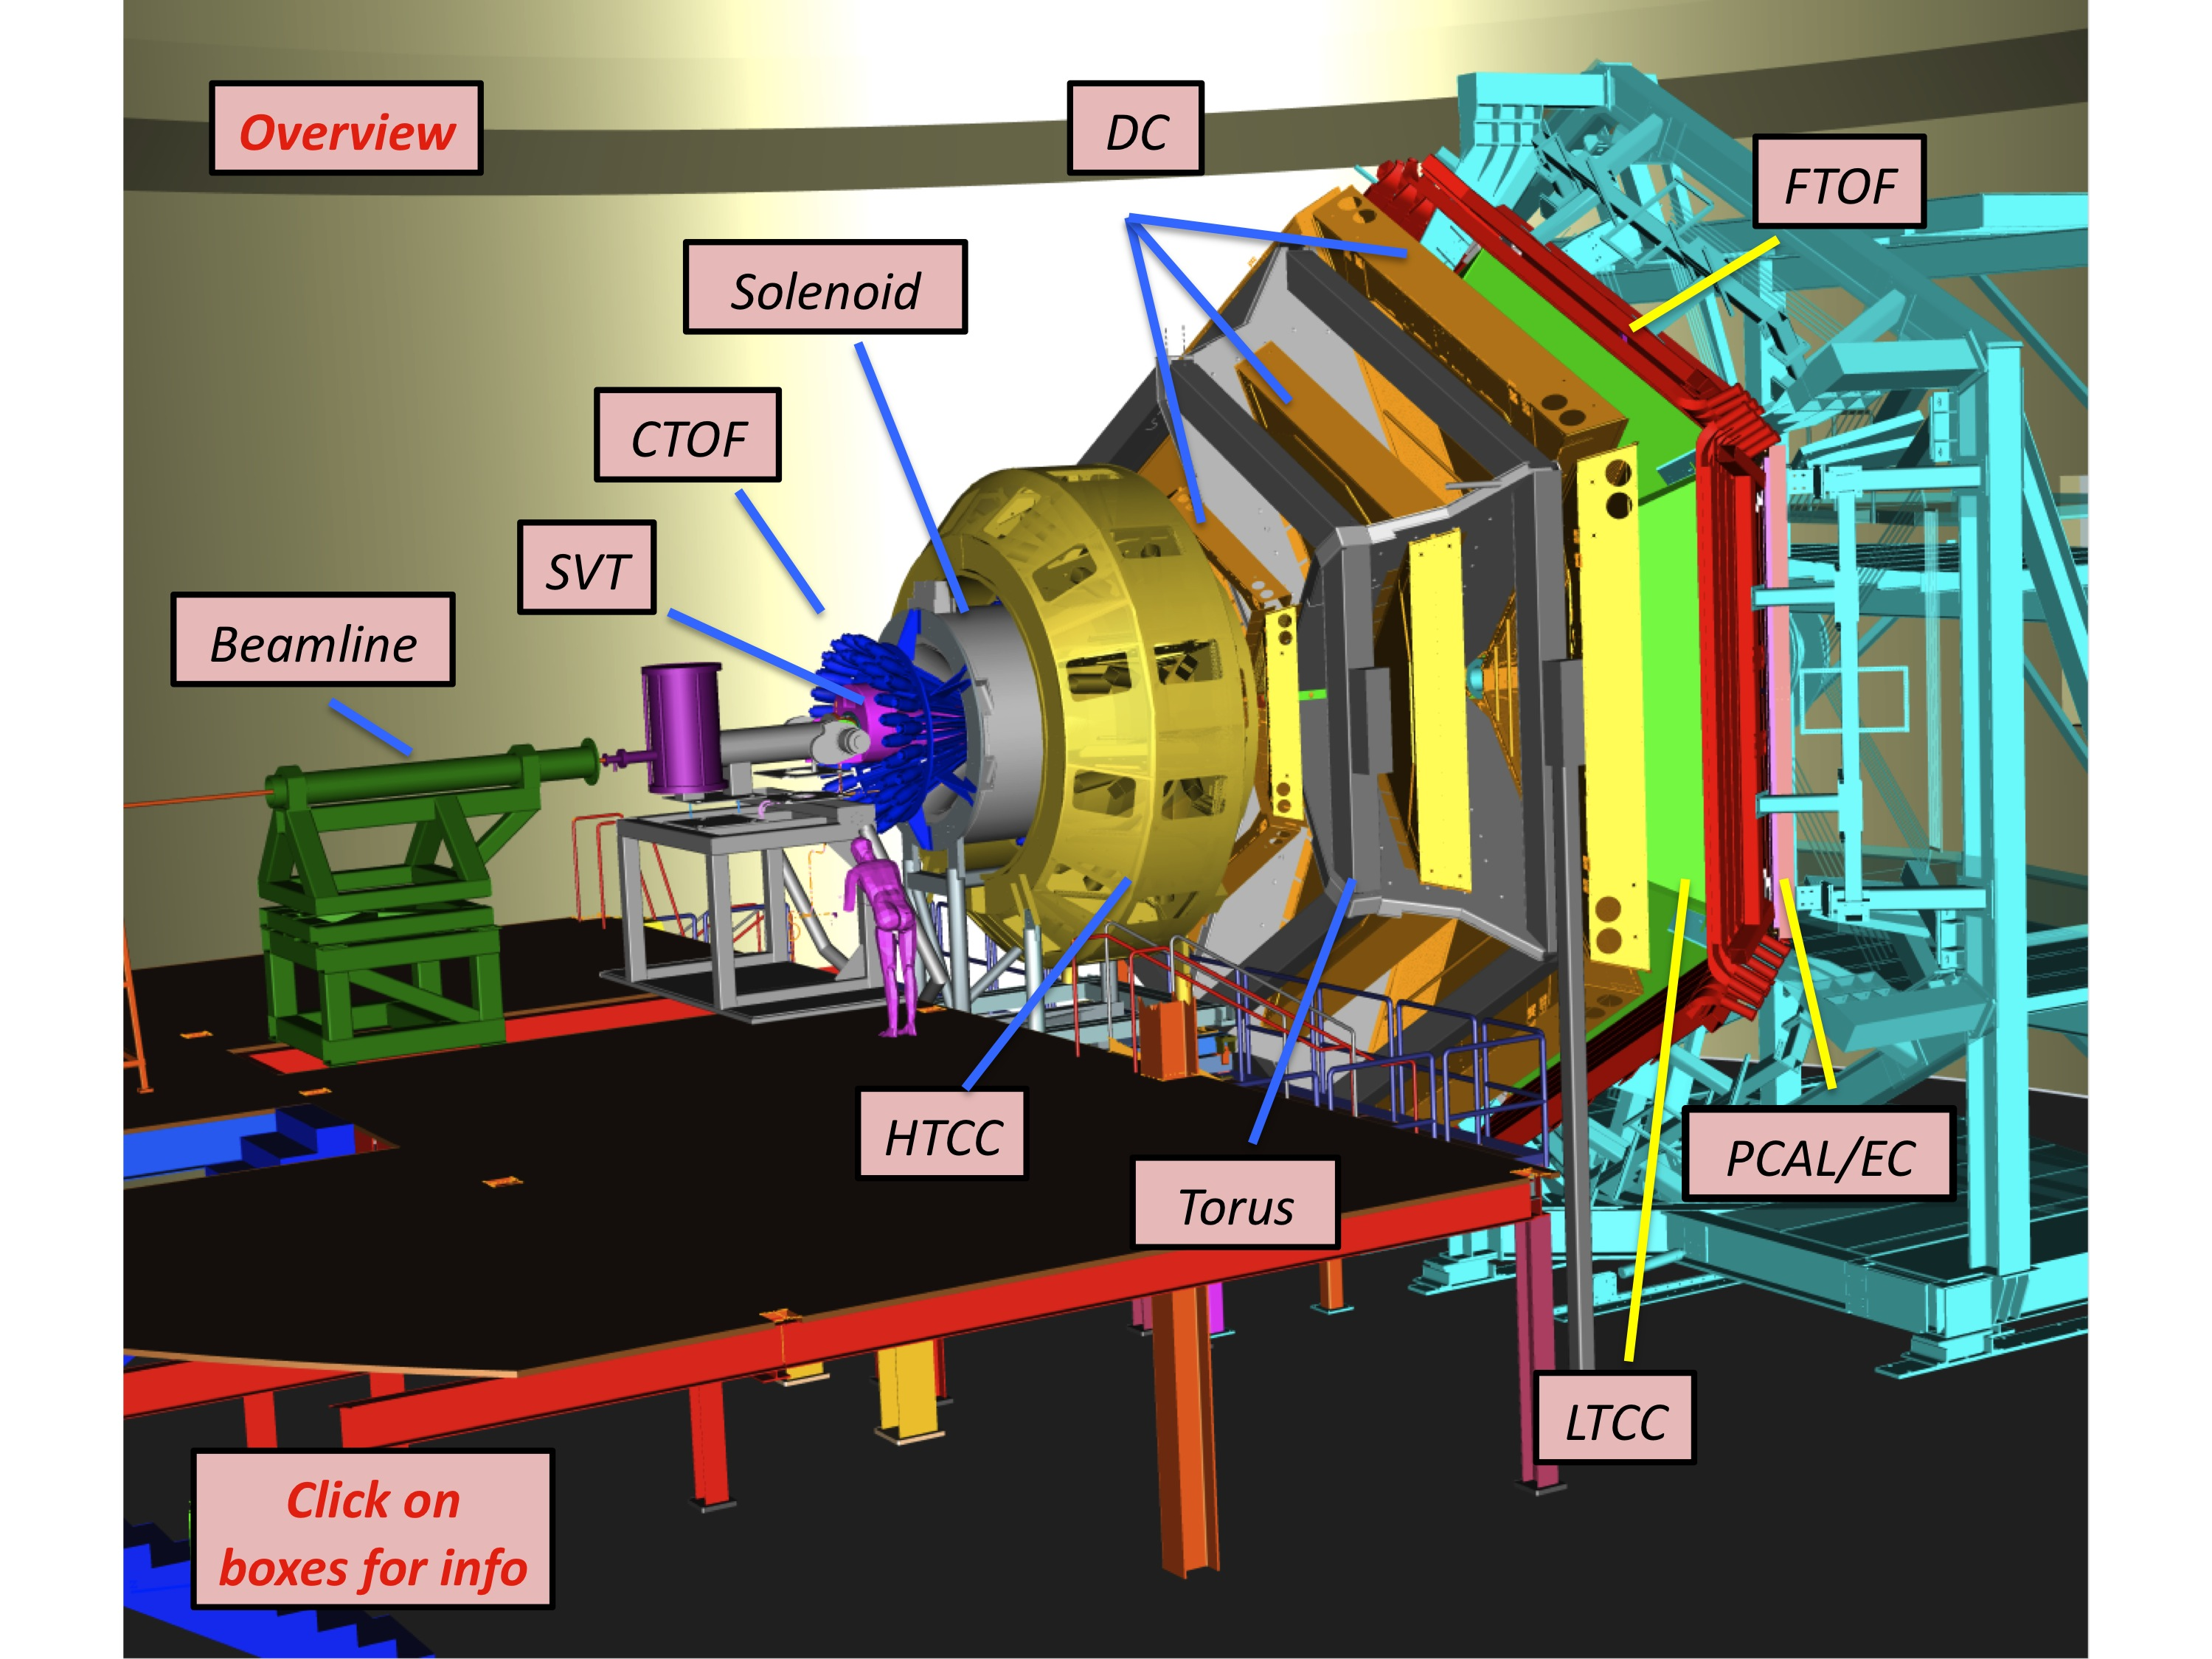
\includegraphics[height=\dimexpr0.5\textheight-0.5in]{Pics/dnp/clas12-overview.jpg}
                    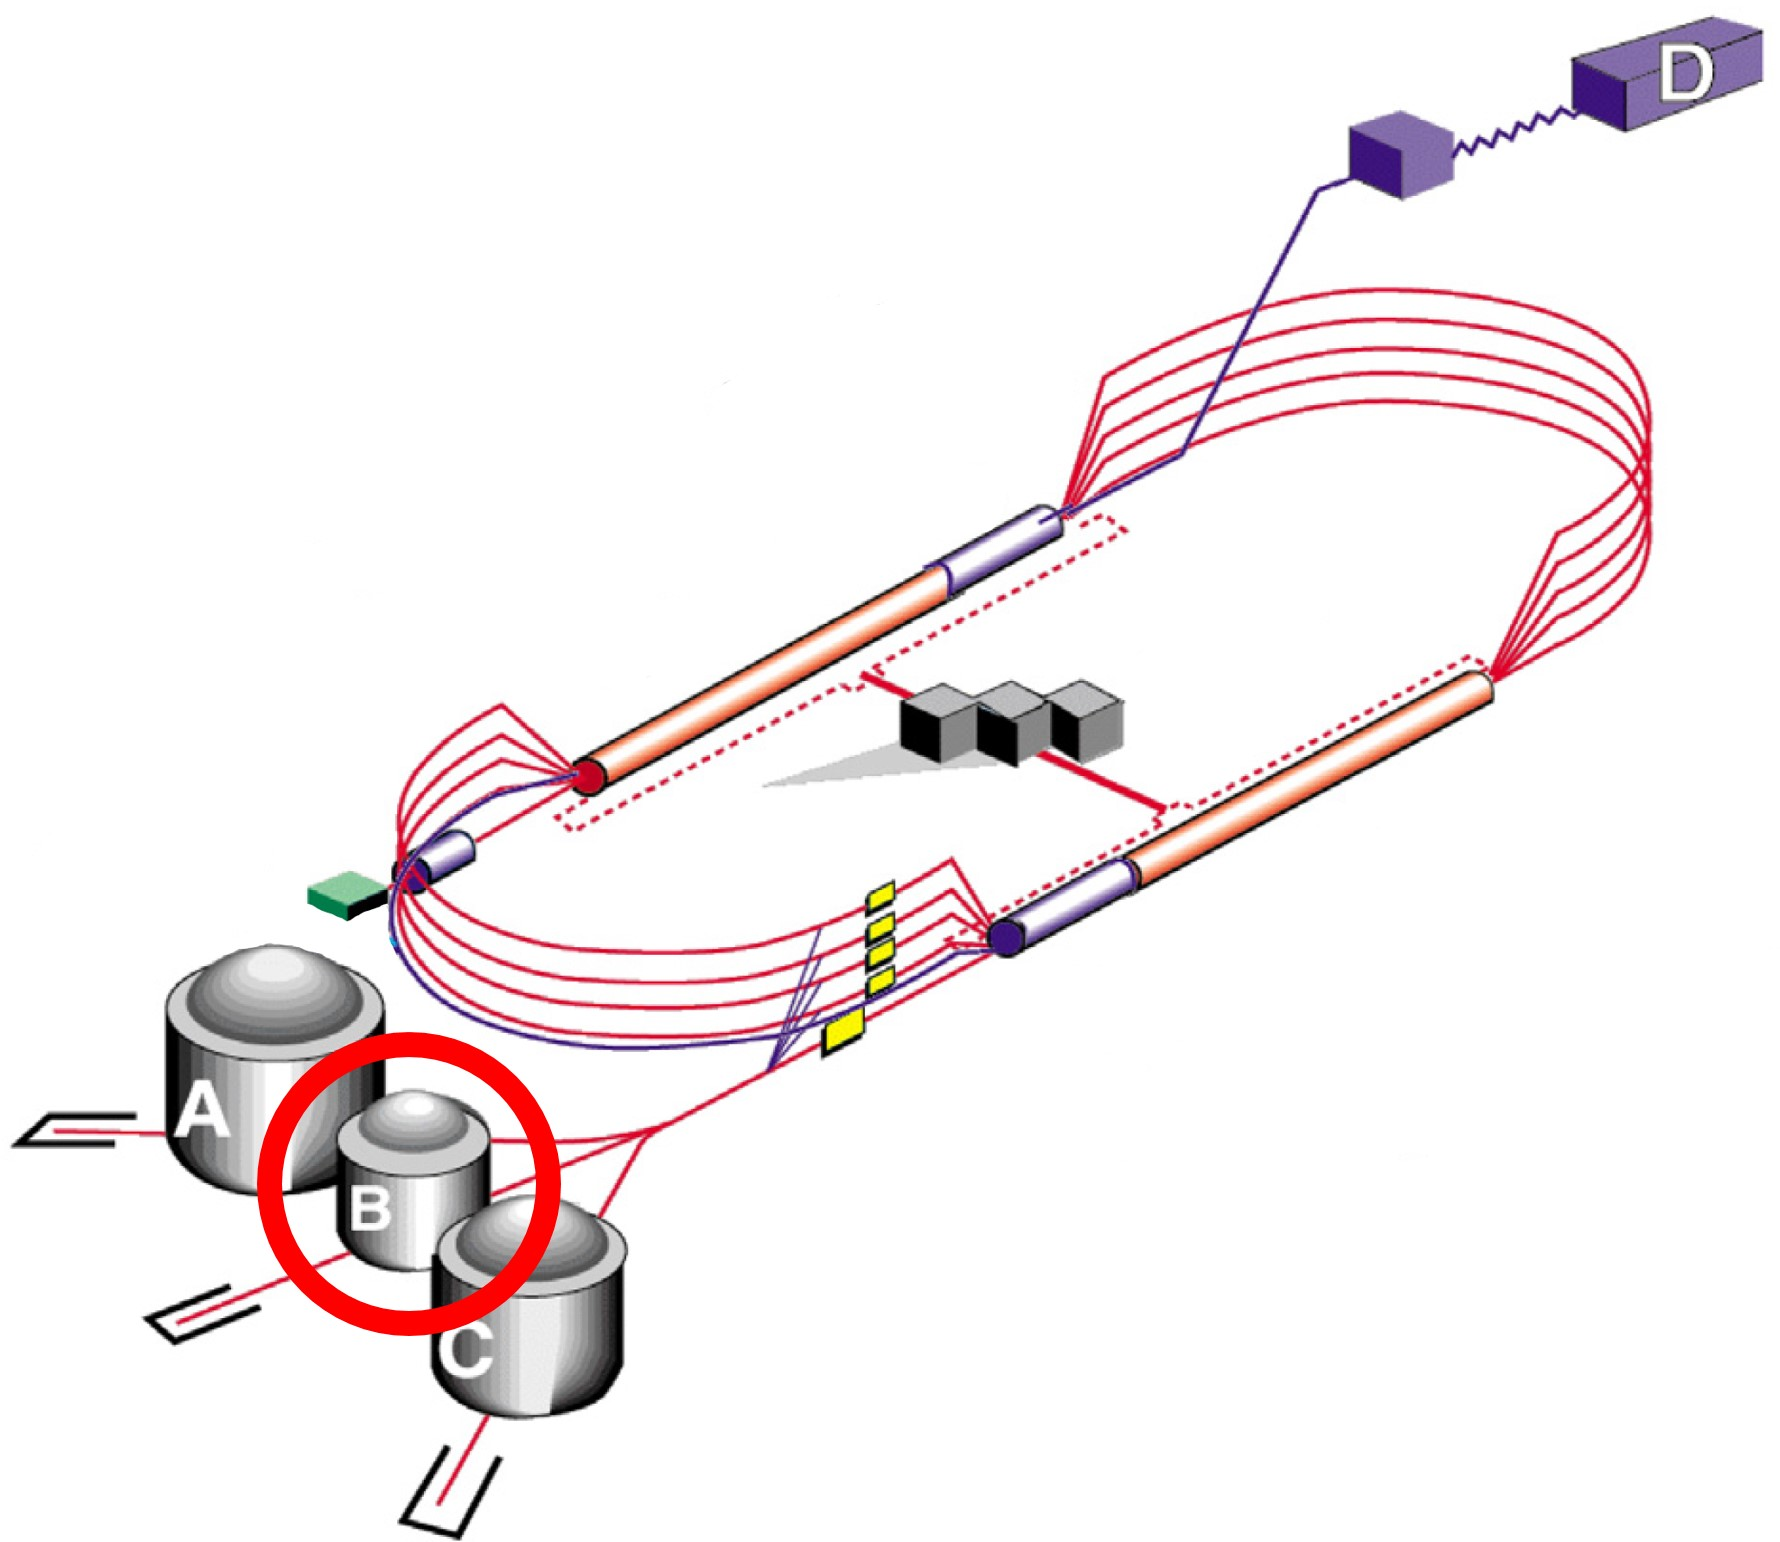
\includegraphics[width=.56765899\textwidth]{DNP/jlab_hall_b_circled.jpg}
                    
                    
                \end{figure}
                \vspace{-0.45cm}
                  \begin{itemize}
                    \setlength\itemsep{1em}
                    \item CEBAF 1,400 m racetrack, 50 RF cryomodules
                    \item 10.6 GeV, $\sim$ 50 nA electron beam
                    \end{itemize}
            
                \vspace{0.3cm}
                {\myfont{\tiny [V. Burkert et al., NIMA, 959, 163419 (2020)] }}
        \end{columns}
\end{frame}    




\begin{frame}{CLAS12 Detector at Jefferson Lab Hall B} 
        \vspace{-0.5cm}
        \begin{columns}[t, onlytextwidth]
            \column{0.5\textwidth}
                %\vspace{1cm}
                \begin{figure}[t!]
                    %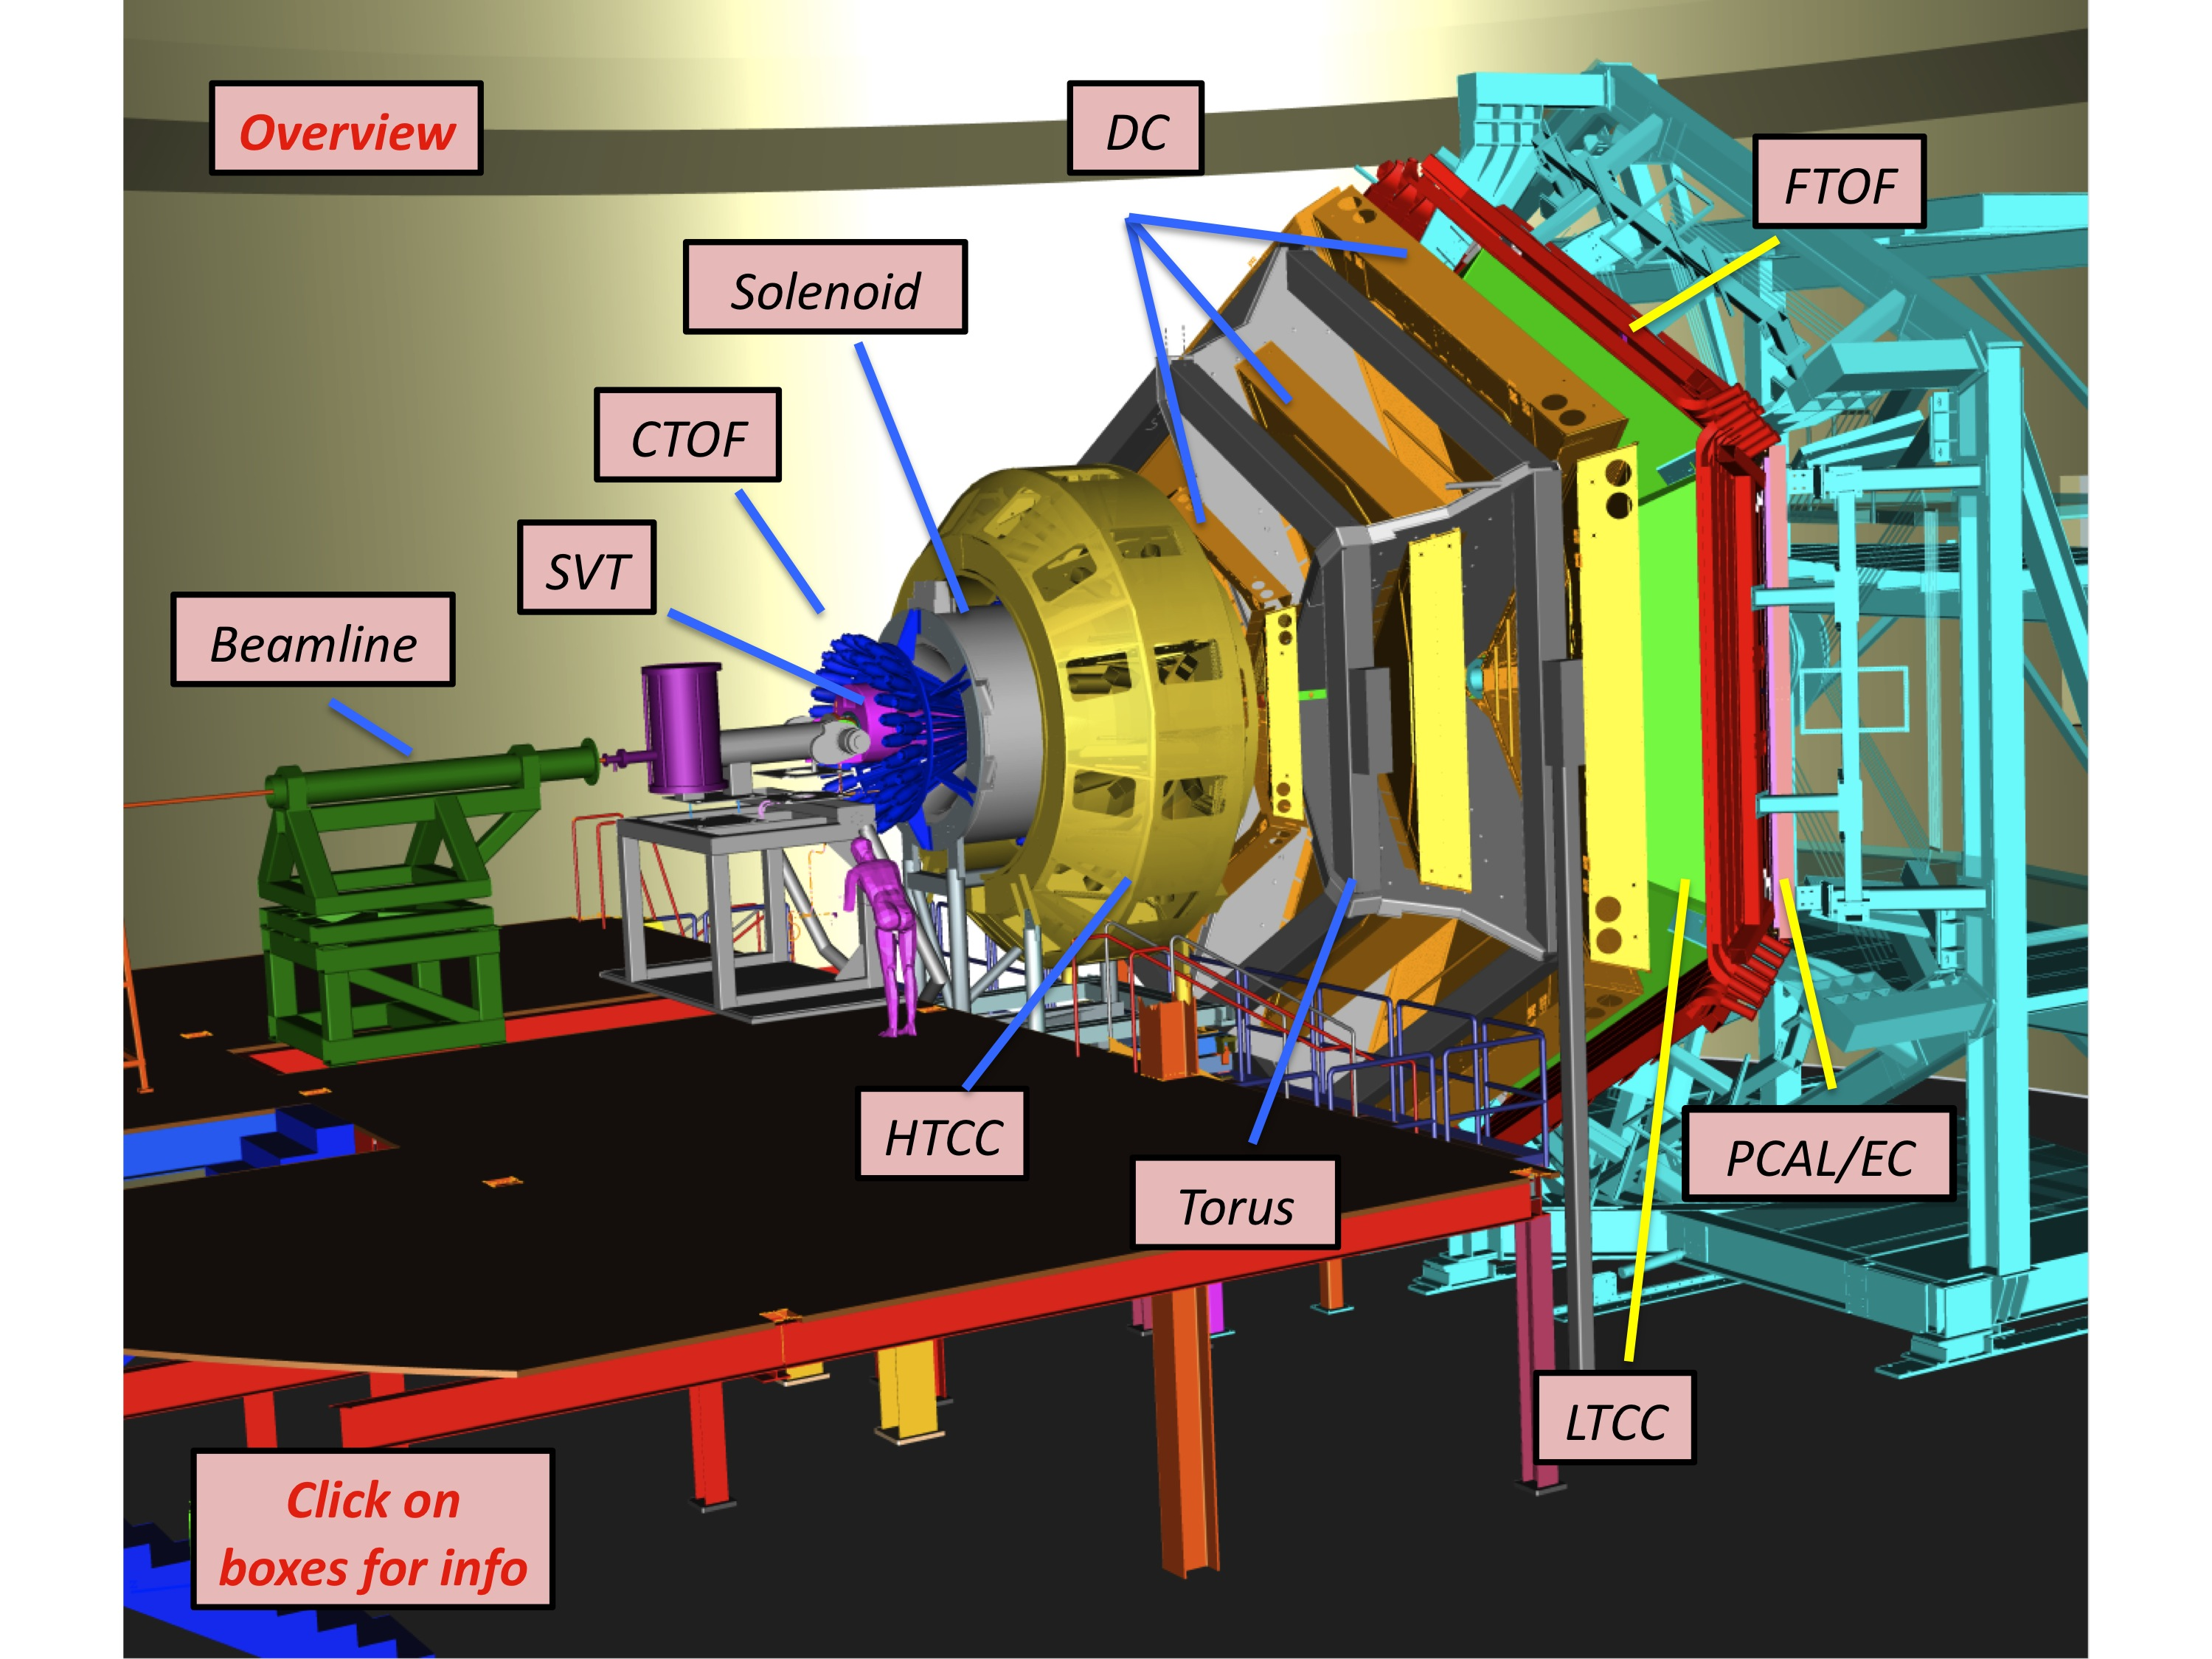
\includegraphics[height=\dimexpr0.5\textheight-0.5in]{Pics/dnp/clas12-overview.jpg}
                    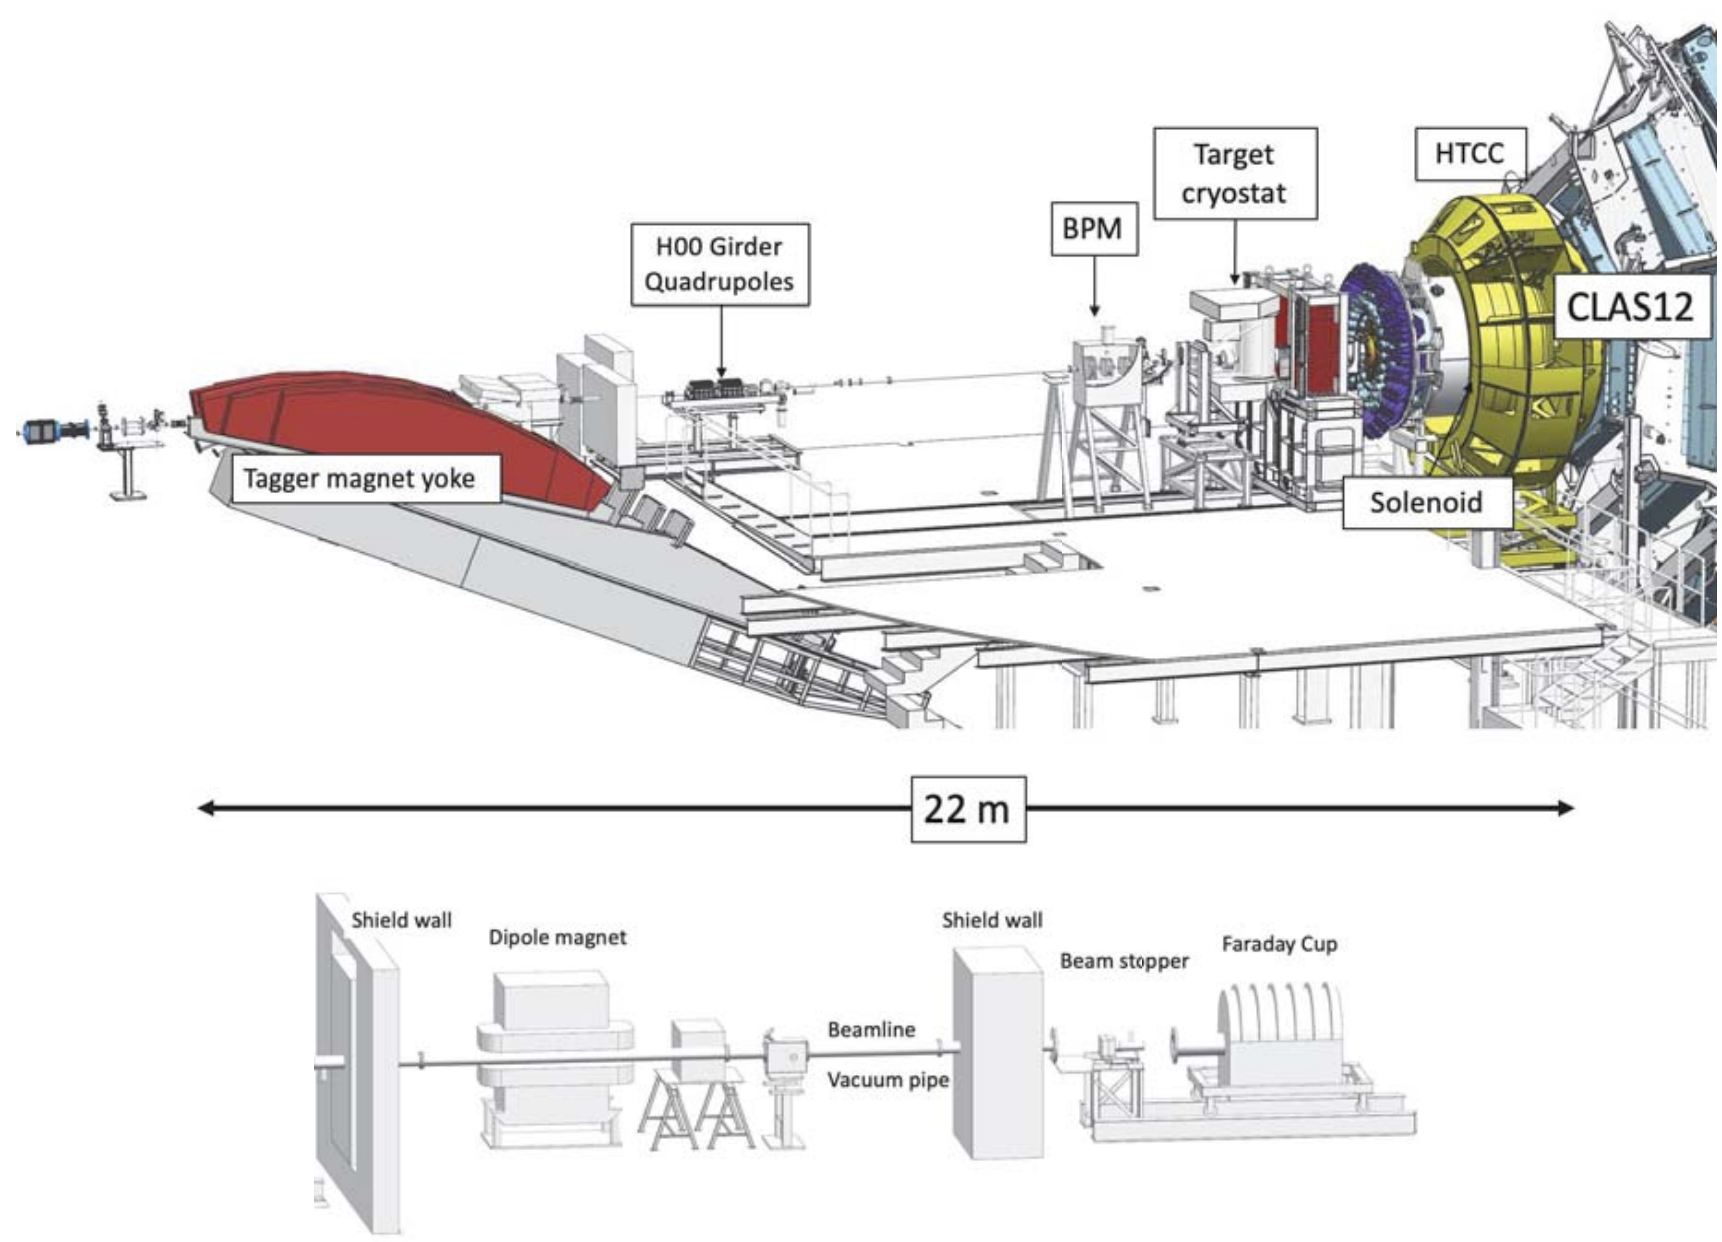
\includegraphics[width=.86349\textwidth]{Main/beamline.png}
                    
                    
                \end{figure}
                \vspace{-0.45cm}
                  \begin{itemize}
                    \setlength\itemsep{1em}
                    \item  Top: Beamline into unpolarized LH$_2$ target (cryostat)
                    \item Bottom: Downstream beamline to Faraday Cup (current monitor)
                    \end{itemize}
                    
            \column{0.5\textwidth}
                \begin{figure}[t!]
                    %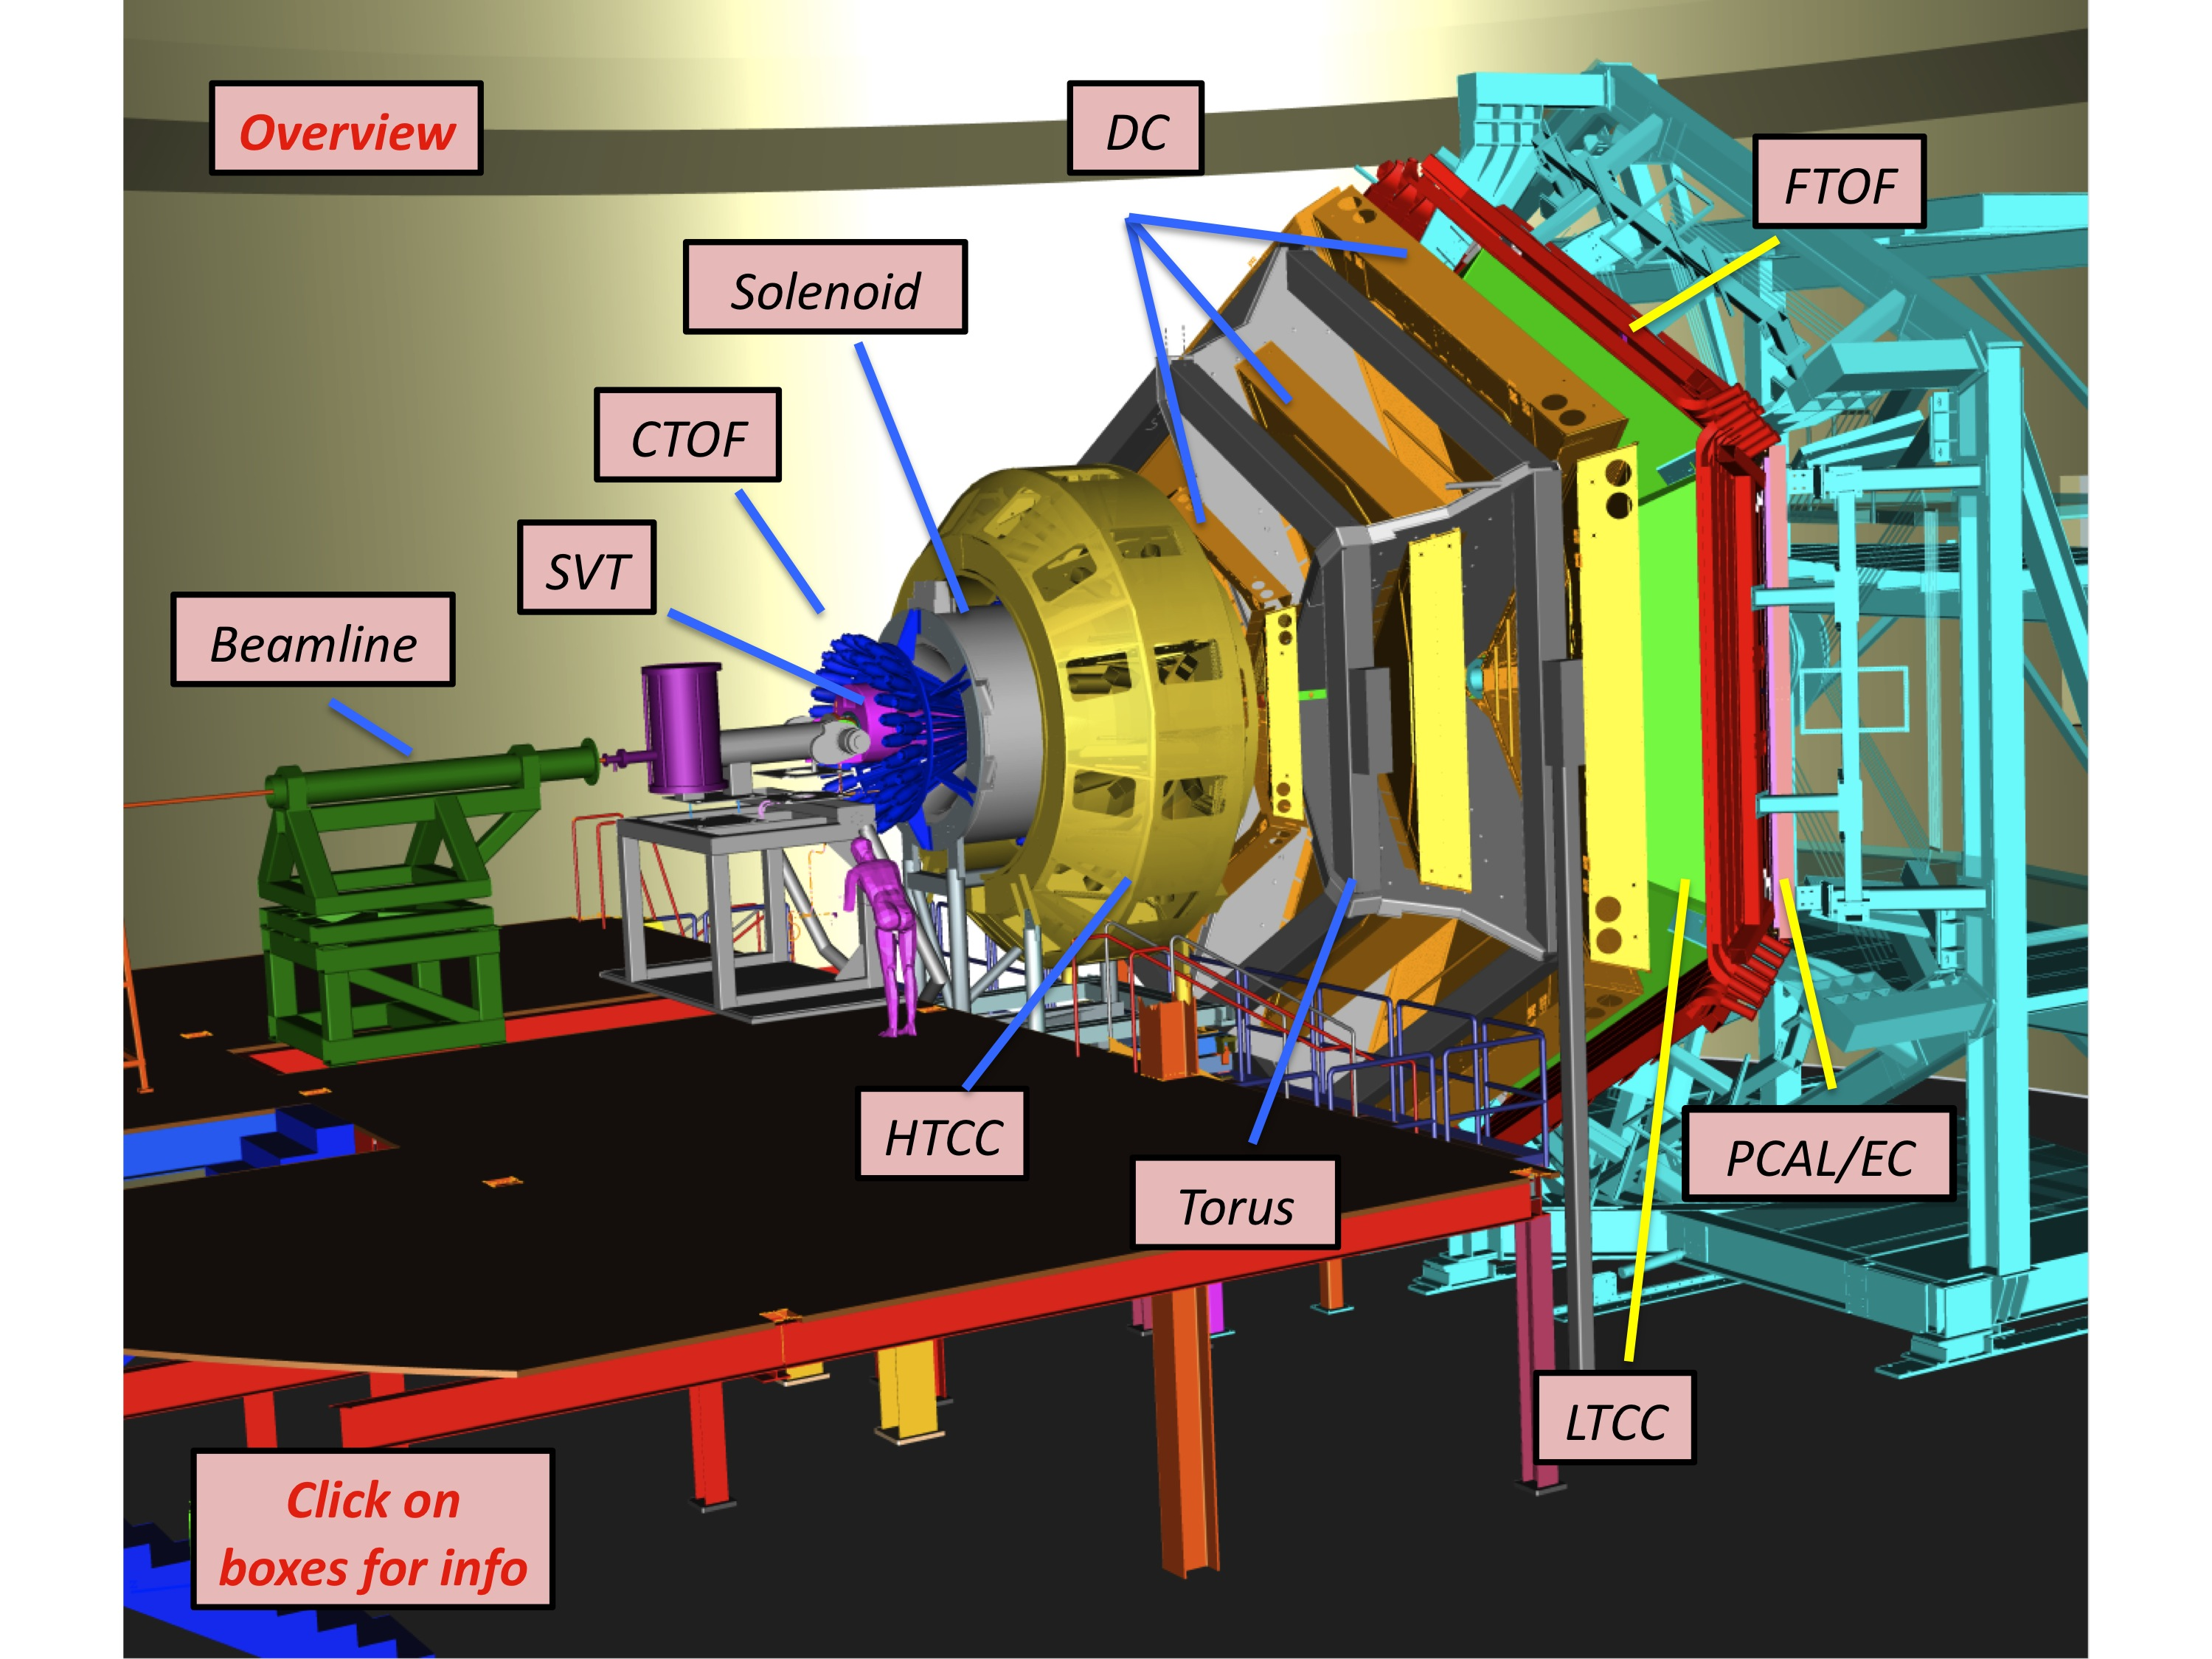
\includegraphics[height=\dimexpr0.5\textheight-0.5in]{Pics/dnp/clas12-overview.jpg}
                    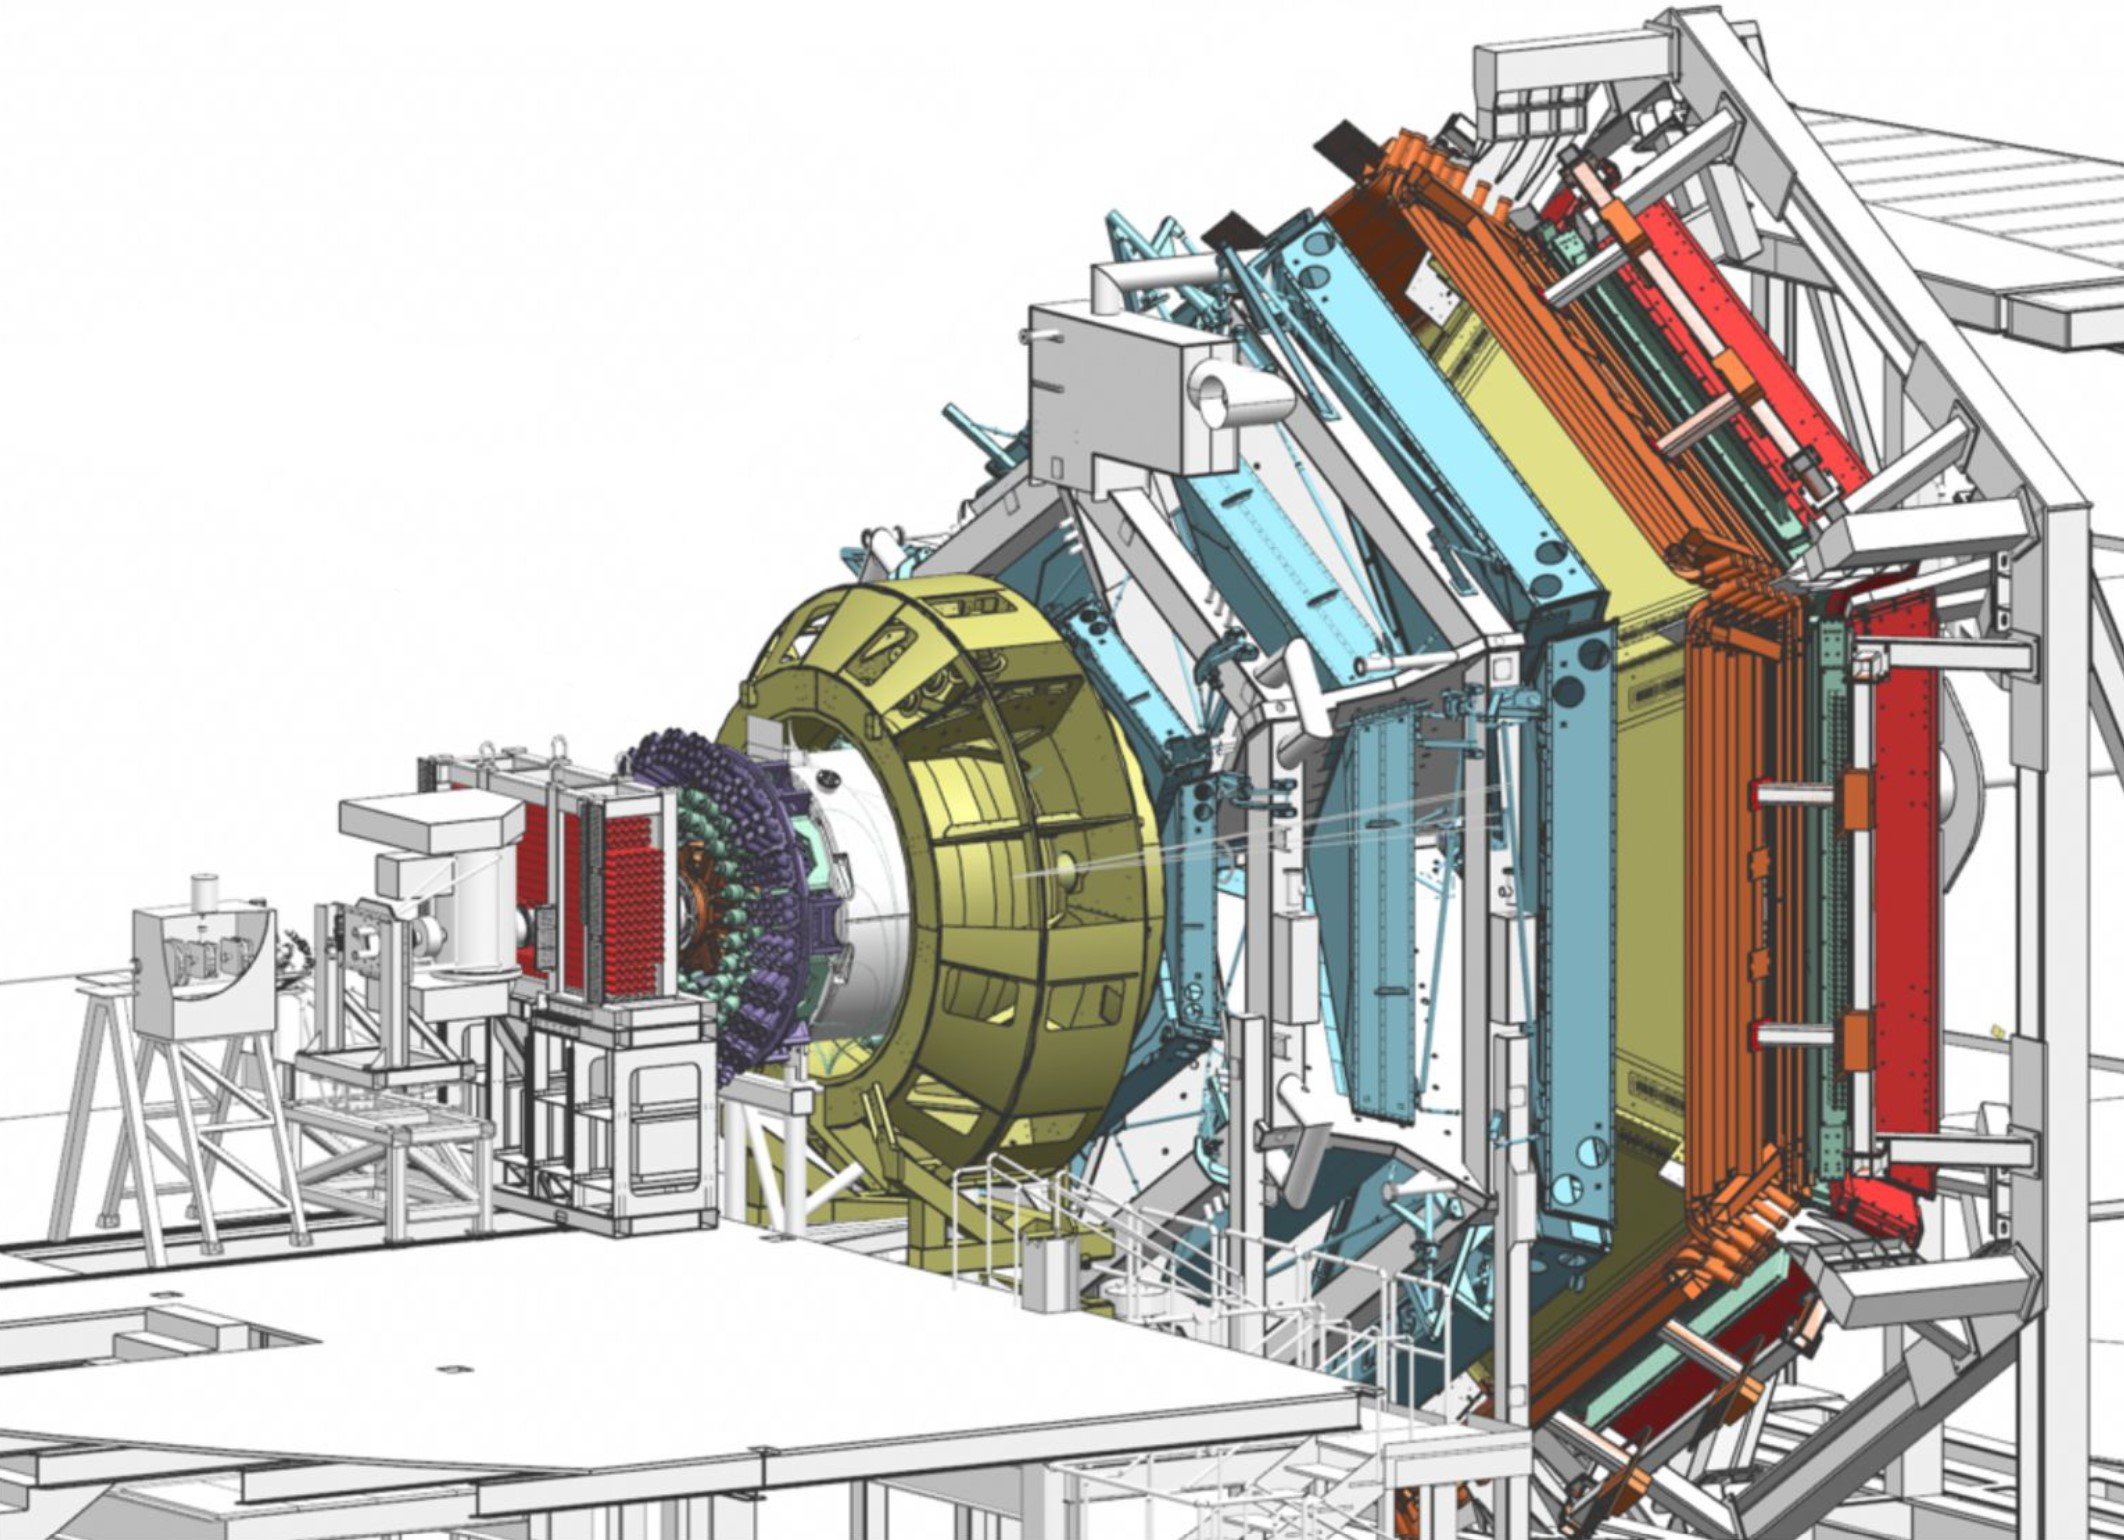
\includegraphics[width=.8565899\textwidth]{DNP/CLASdetector.jpg}
                    
                    
                \end{figure}
                \vspace{-0.45cm}
                \begin{itemize}
                    \setlength\itemsep{1em}

                    \item CEBAF Large Acceptance Spectrometer:\\
                     \begin{itemize}
                            \item $\sim$ 2$\pi$ coverage in $\phi$\\
                        \item  $5^\circ$ - $125^\circ$ coverage in $\theta$
                        \item Full 4 particle final state reconstruction for this process
                    \end{itemize}
                    
                    
                \end{itemize}
                %\vspace{0.3cm}
                {\myfont{\tiny [V. Burkert et al., NIMA, 959, 163419 (2020)] }}
        \end{columns}
\end{frame}    


\begin{frame}{Experiment Layout And Particle Detection} \label{frame:datasets3}
\vspace{-0.5cm}
        \begin{columns}[t, onlytextwidth]
            \column{0.55\textwidth}
                \begin{itemize}
                    \setlength\itemsep{.35em}
                    \item 6-fold symmetric Forward Detector ($\theta < \sim 40 ^{\circ}$) with torodial field
                     \begin{itemize}
                    \setlength\itemsep{.25em}
                        \item Cherenkov Counters
                        \item Drift Chambers
                        \item Time-of-Flight Detectors
                        \item EM Calorimeters
                    \end{itemize}
                      \item Central Detector ($\sim40^{\circ} < \theta < \sim 125 ^{\circ}$) \\
                      inside solenoid
                     \begin{itemize}
                    \setlength\itemsep{.25em}
                        \item Silicon Vertex Tracker
                        \item Micromegas
                        \item ToF Detector

                    \end{itemize}
                    
                    \item Forward Tagger, Backward Angle Neutron Detector
                    \item Faraday Cup for luminosity measurement
                
            
                \end{itemize}
            
                \vspace{0.1cm}
                
            \column{0.45\textwidth}
                %\vspace{1cm}
                \vspace{0.3cm}
                \begin{figure}[t!]
                    %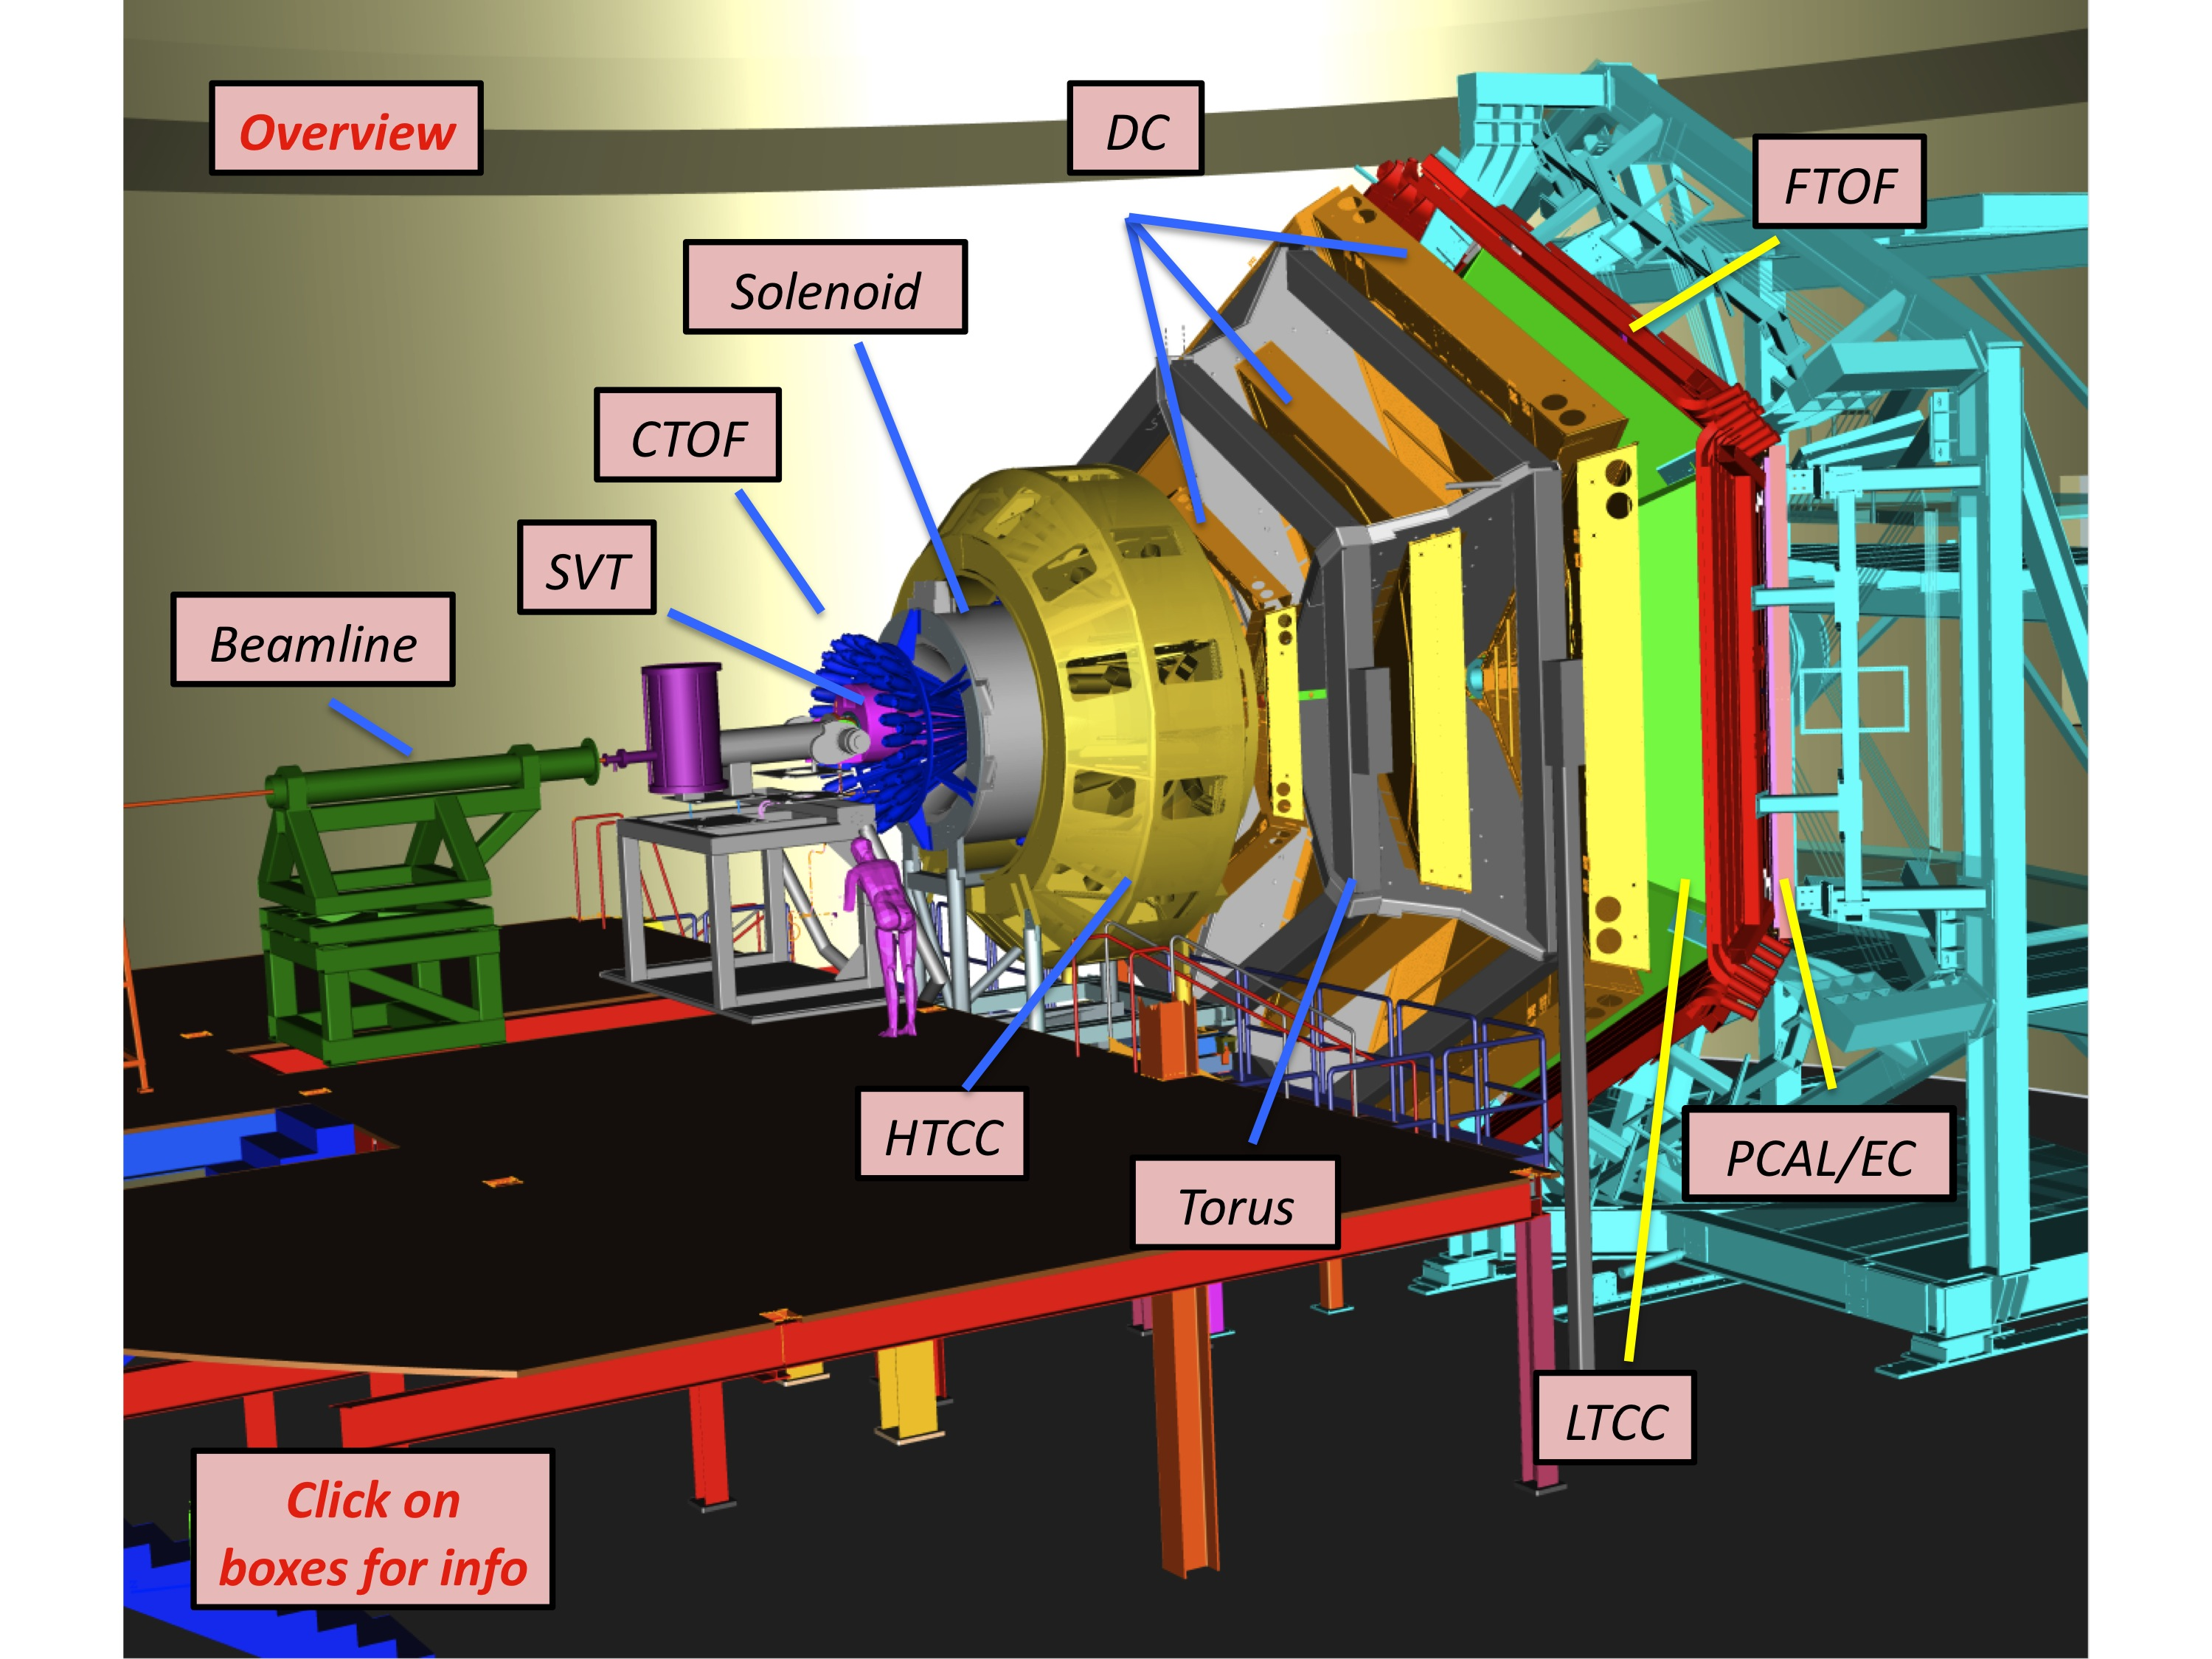
\includegraphics[height=\dimexpr0.5\textheight-0.5in]{Pics/dnp/clas12-overview.jpg}
                    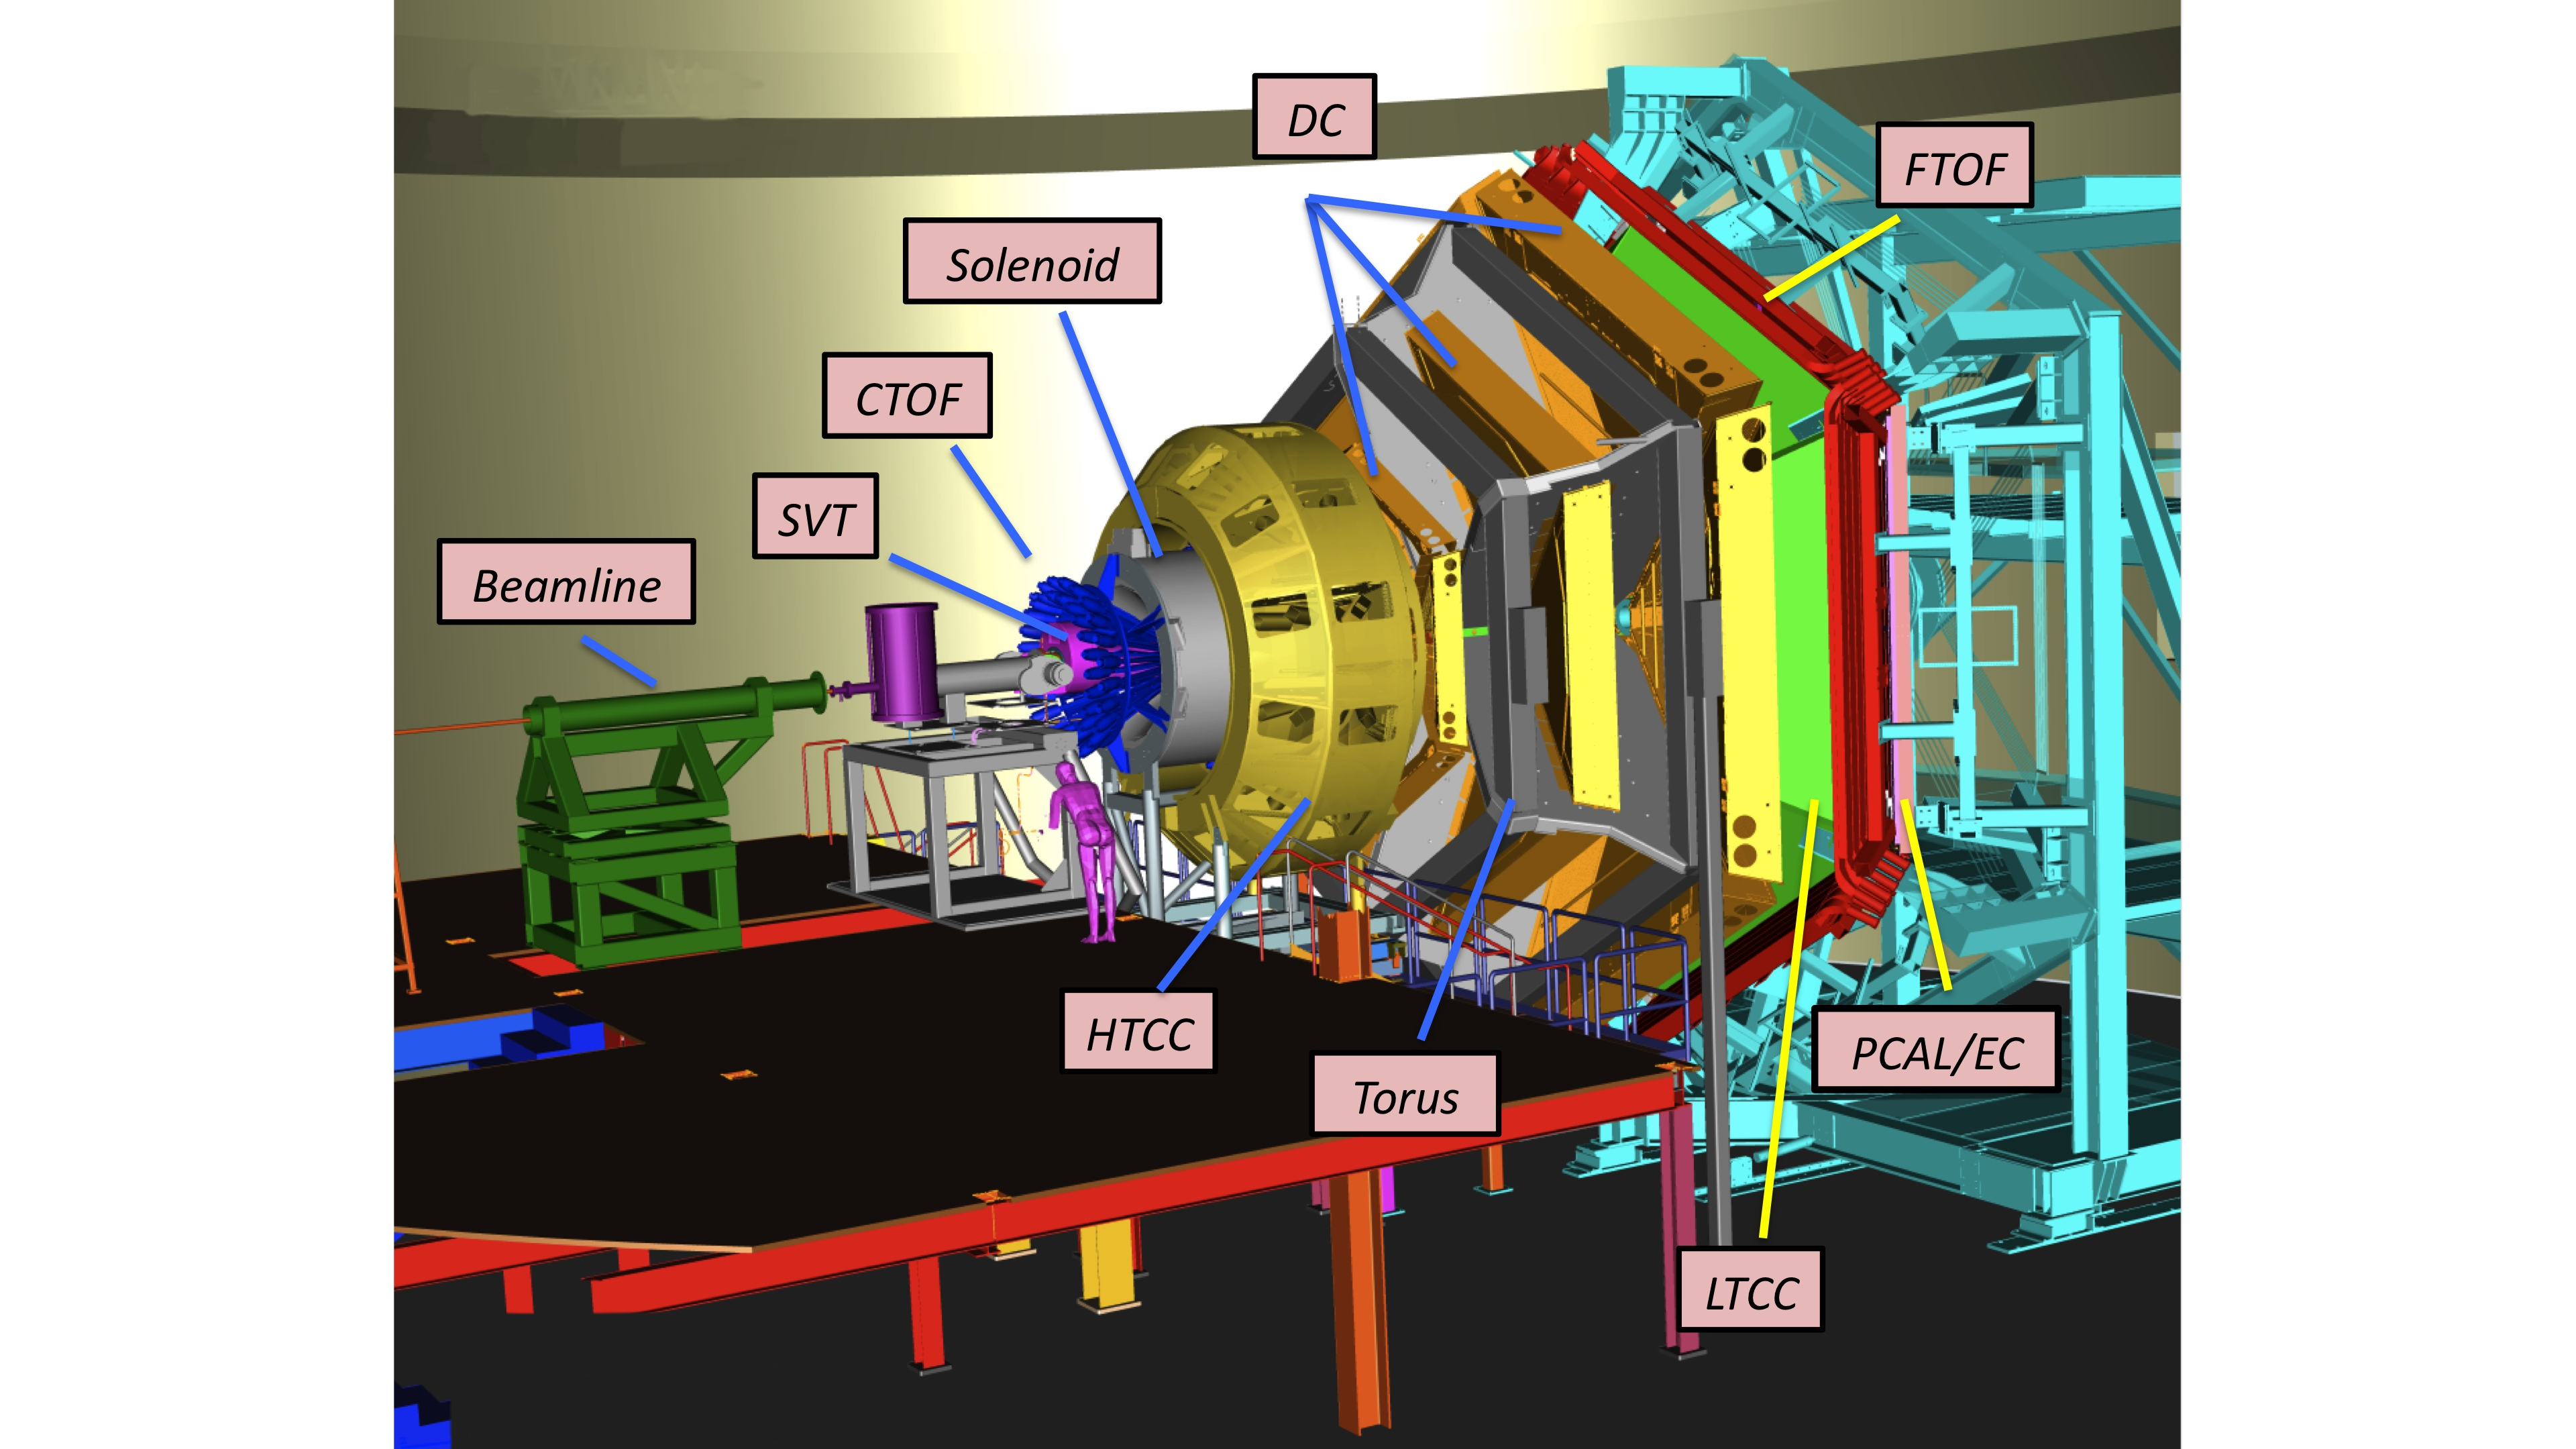
\includegraphics[trim={8cm 1cm  8cm 1cm},width=.899\textwidth]{DNP/jlab_clas_layout_1.png}
                    

                    
                \end{figure}
                \begin{itemize}
                    \setlength\itemsep{.35em}
                    \item This analysis examines data taken in Fall 2018
                    \end{itemize}
                {\myfont{\tiny [V. Burkert et al., NIMA, 959, 163419 (2020)] }}
        \end{columns}
\end{frame}    


\begin{frame}{Components of Cross Section}

    
    \begin{figure}[h]
        \centering
        \begin{tikzpicture}
            \node[anchor=south west,inner sep=0] at (0,0) {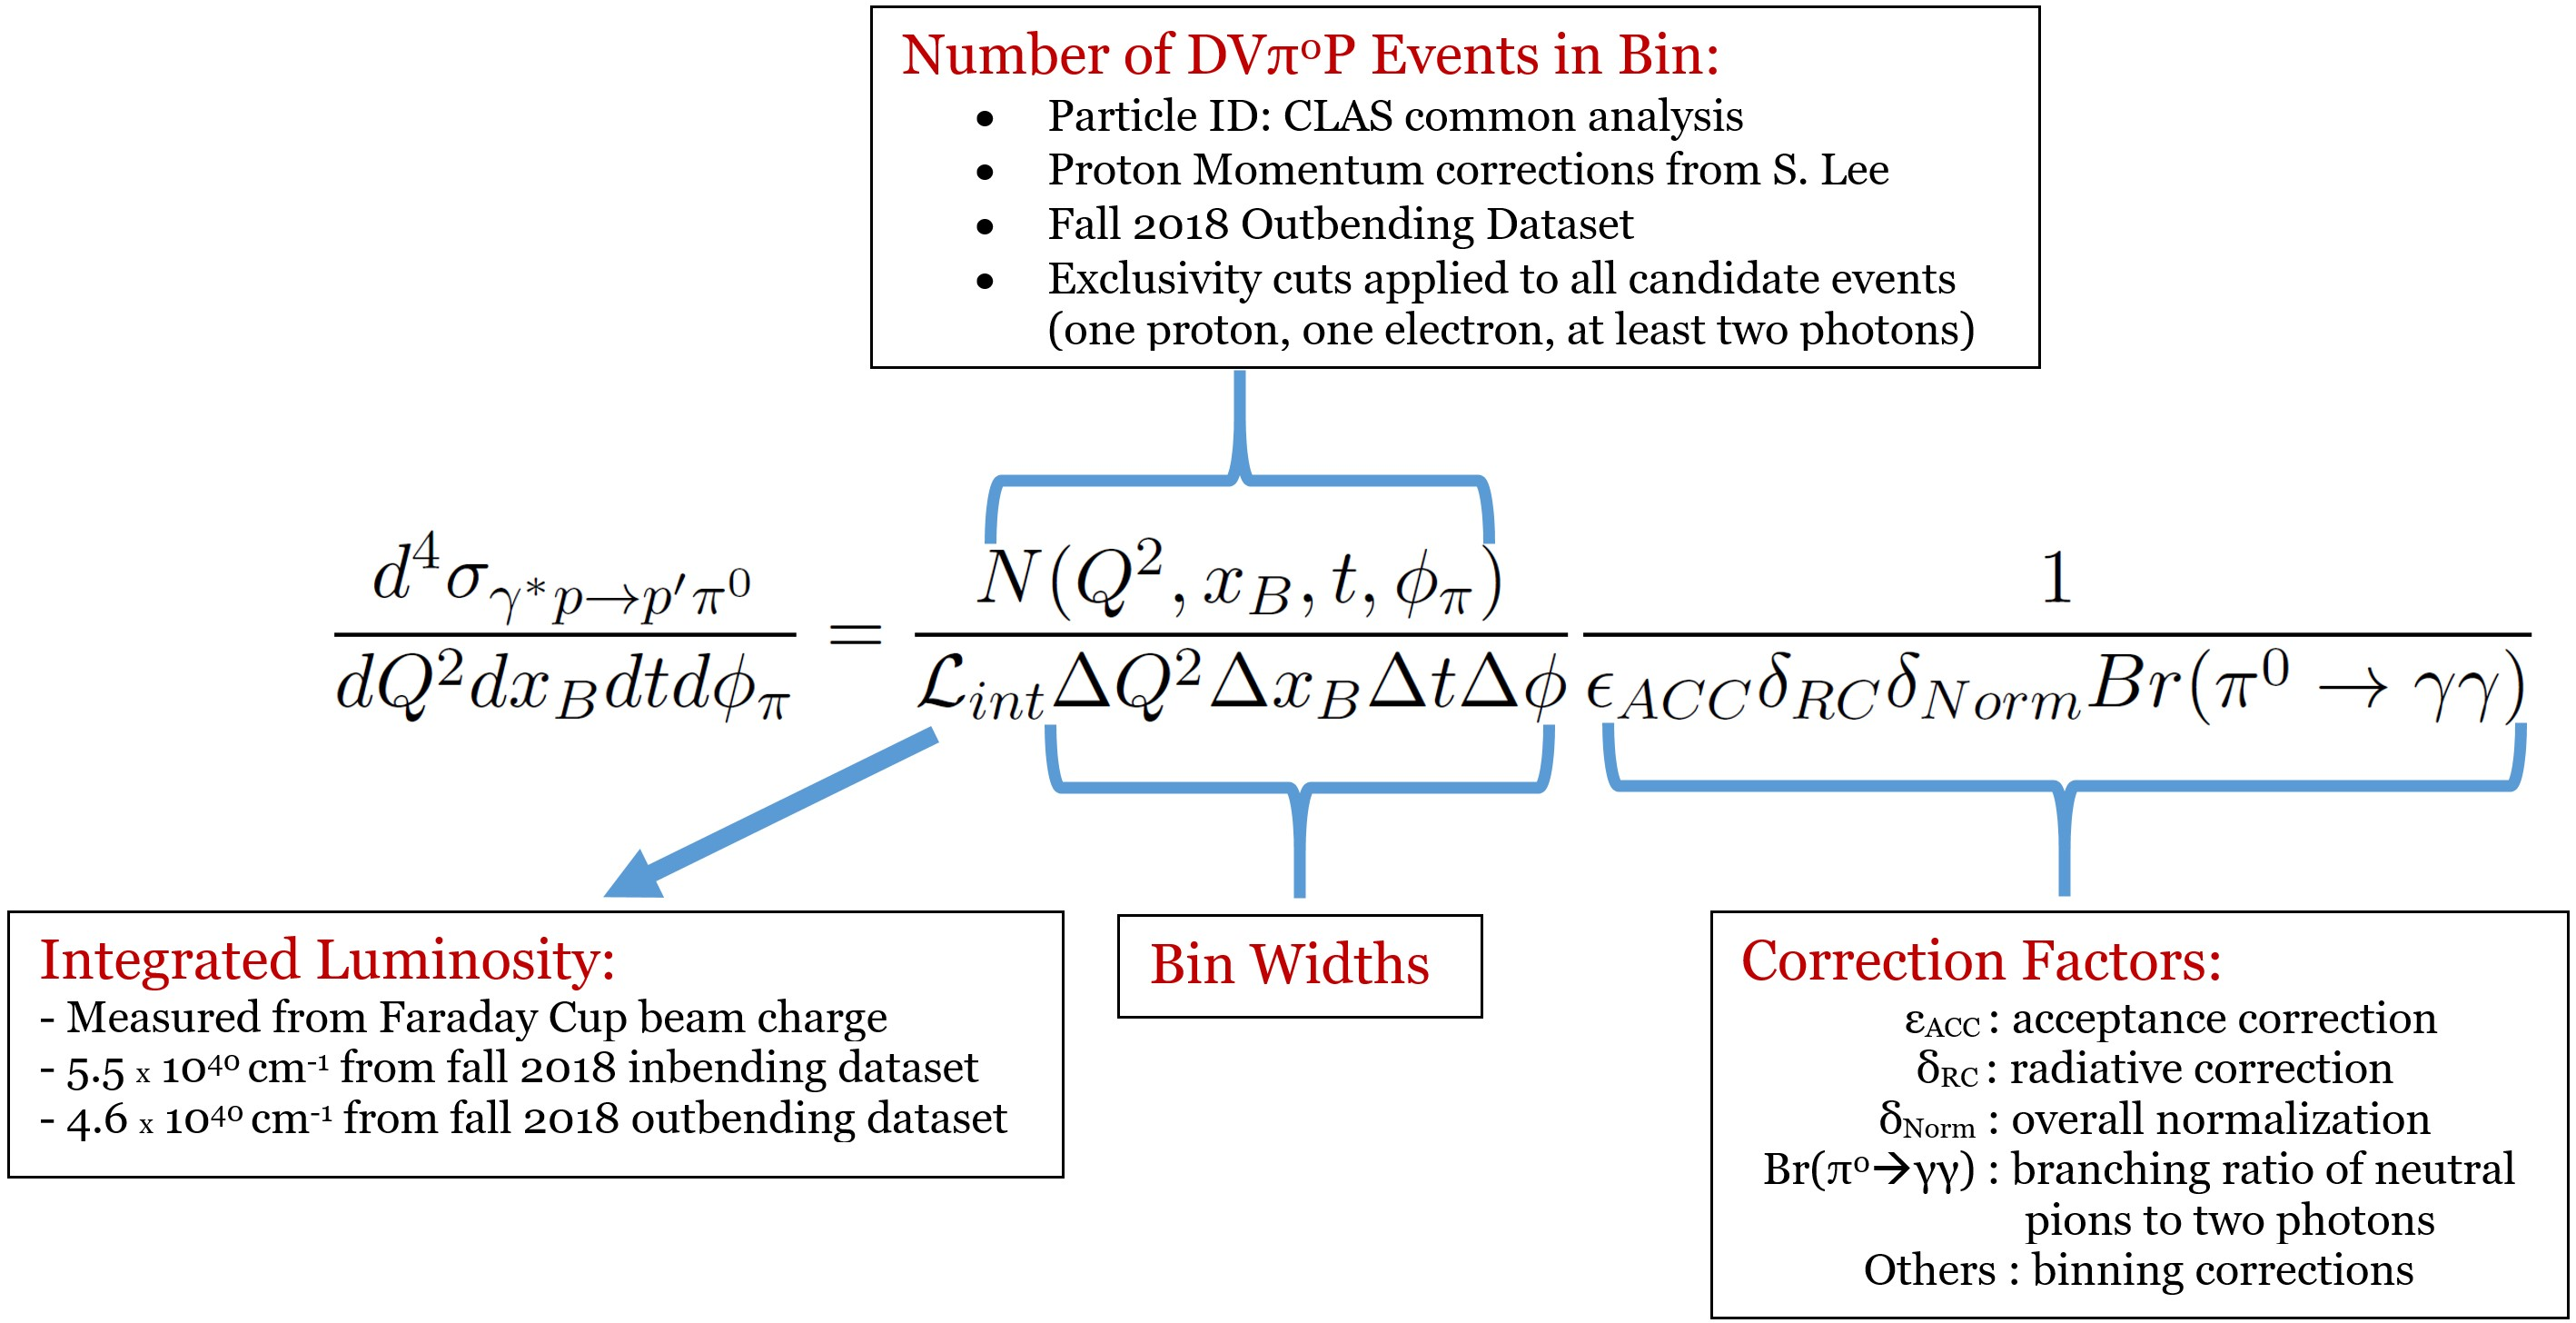
\includegraphics[trim={0 0  0 0cm} ,clip,width=.791725995\textwidth]{extra/steps3.jpg}};
            % The overlayed rectangle
            \fill[green, opacity=0] (4.5cm,3.25cm) rectangle (7cm,3.65cm);
        \end{tikzpicture}
    \end{figure}
\end{frame}






\begin{frame}{Components of Cross Section: Luminosity}
    \begin{figure}[h]
        \centering
        \begin{tikzpicture}
            \node[anchor=south west,inner sep=0] at (0,0) {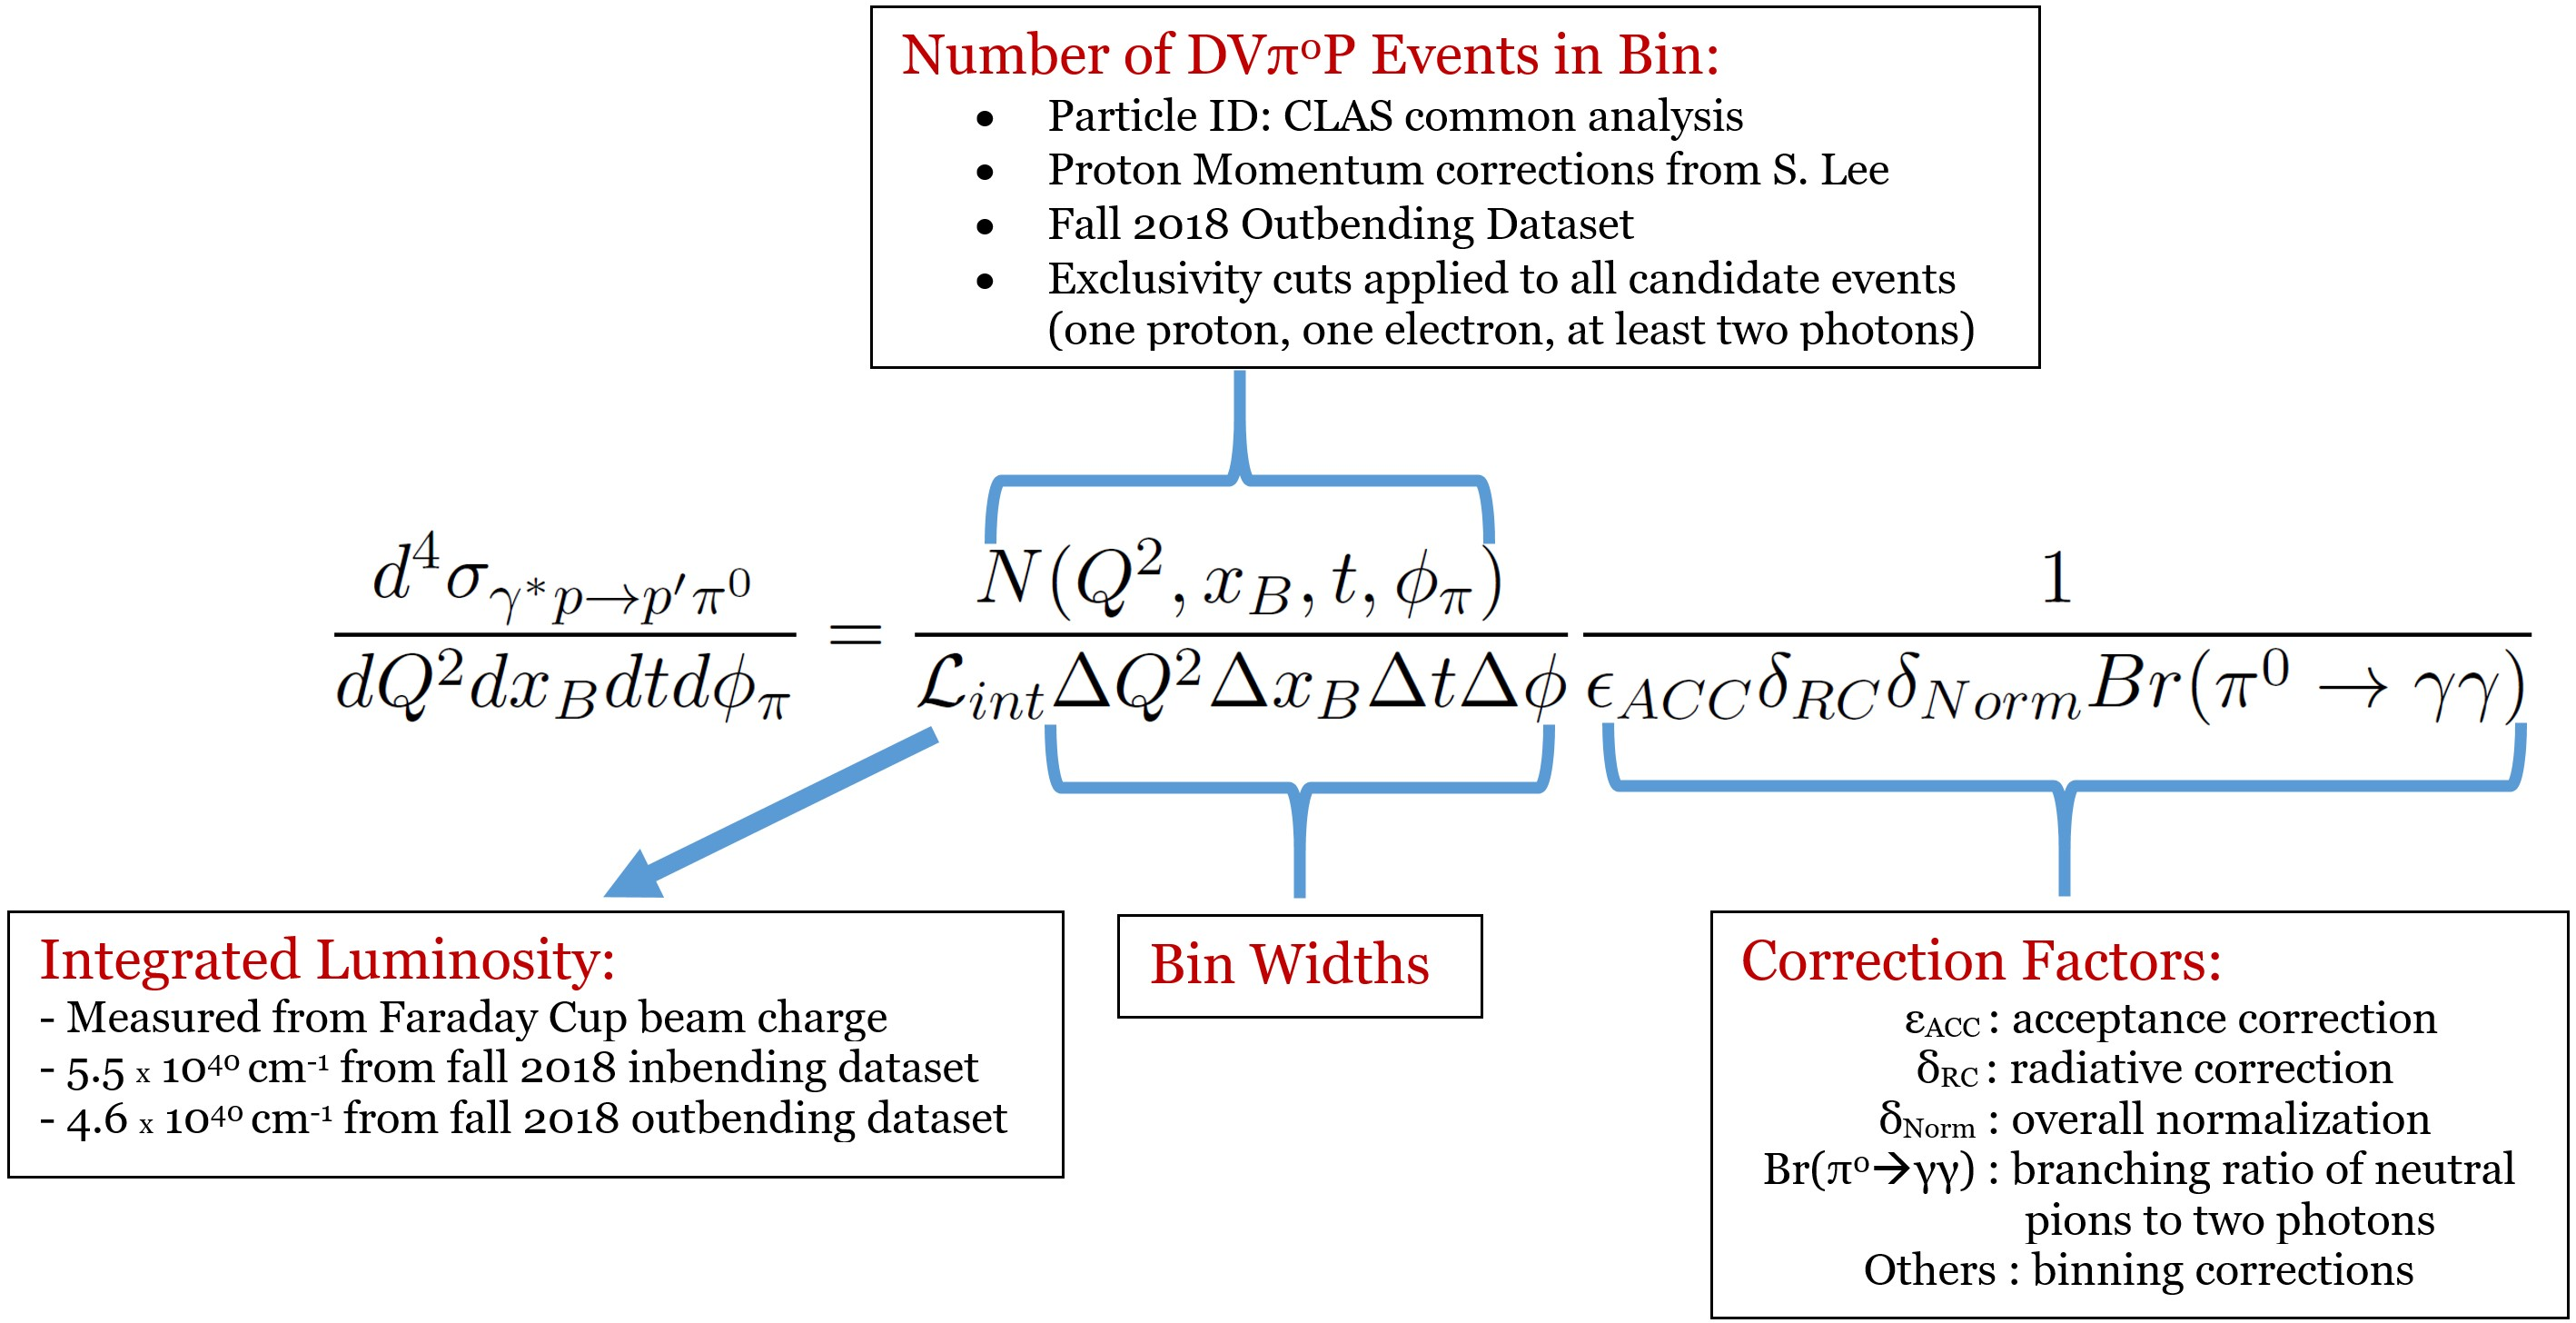
\includegraphics[trim={0 0  0 0cm} ,clip,width=.791725995\textwidth]{extra/steps3.jpg}};
            % The overlayed rectangle
            \fill[green, opacity=0.25] (4.2cm,2.75cm) rectangle (4.85cm,3.15cm);
        \end{tikzpicture}
    \end{figure}
\end{frame}

\begin{frame}{ Luminosity Determination}
         \begin{equation*}
                    \Lumi = \frac{N_A l \rho Q_{FCUP}}{e}
        \end{equation*}
        
        \begin{columns}
                                
            \column{0.58\textwidth}
                \begin{table}
                    \centering
                    \begin{tabular}{rcc}
                         %& Heading 1 & Heading 2 \\\hline
                        Quantity &  & CLAS12 Value \\\hline
                       Avogadro's Number &  N$_A$  & $6x10^{23}$ \\
                        Electron Charge &e  &  $1.6x10^{-19}$ \\
                        Target Length &l &  5 cm \\
                        Target Density &$\rho$  &  0.07 $g/cm^3$ (LH2) \\
                        Charge on Faraday Cup & $Q_{FCUP}$ &  In data\\
                    \end{tabular}
                    \label{tab:demo}
                \end{table}

            \column{0.42\textwidth}
                \begin{figure}
                    \centering
                    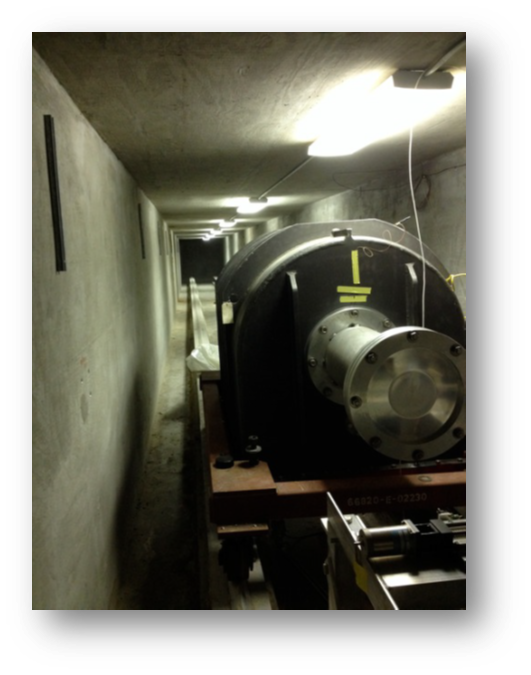
\includegraphics[width=0.6\textwidth]{defense/beamdump1.png}
                    \caption{Caption}
                    \label{fig:enter-label}
                \end{figure}
            
        \end{columns}
       Calculated Integrated Luminosity from Fall 2018  dataset: 5.512 e+40 $cm^{-2}$ inbending, 4.652 e+40 $cm^{-2}$ outbending
\end{frame}    



\begin{frame}{Components of Cross Section}
    \begin{figure}[h]
        \centering
        \begin{tikzpicture}
            \node[anchor=south west,inner sep=0] at (0,0) {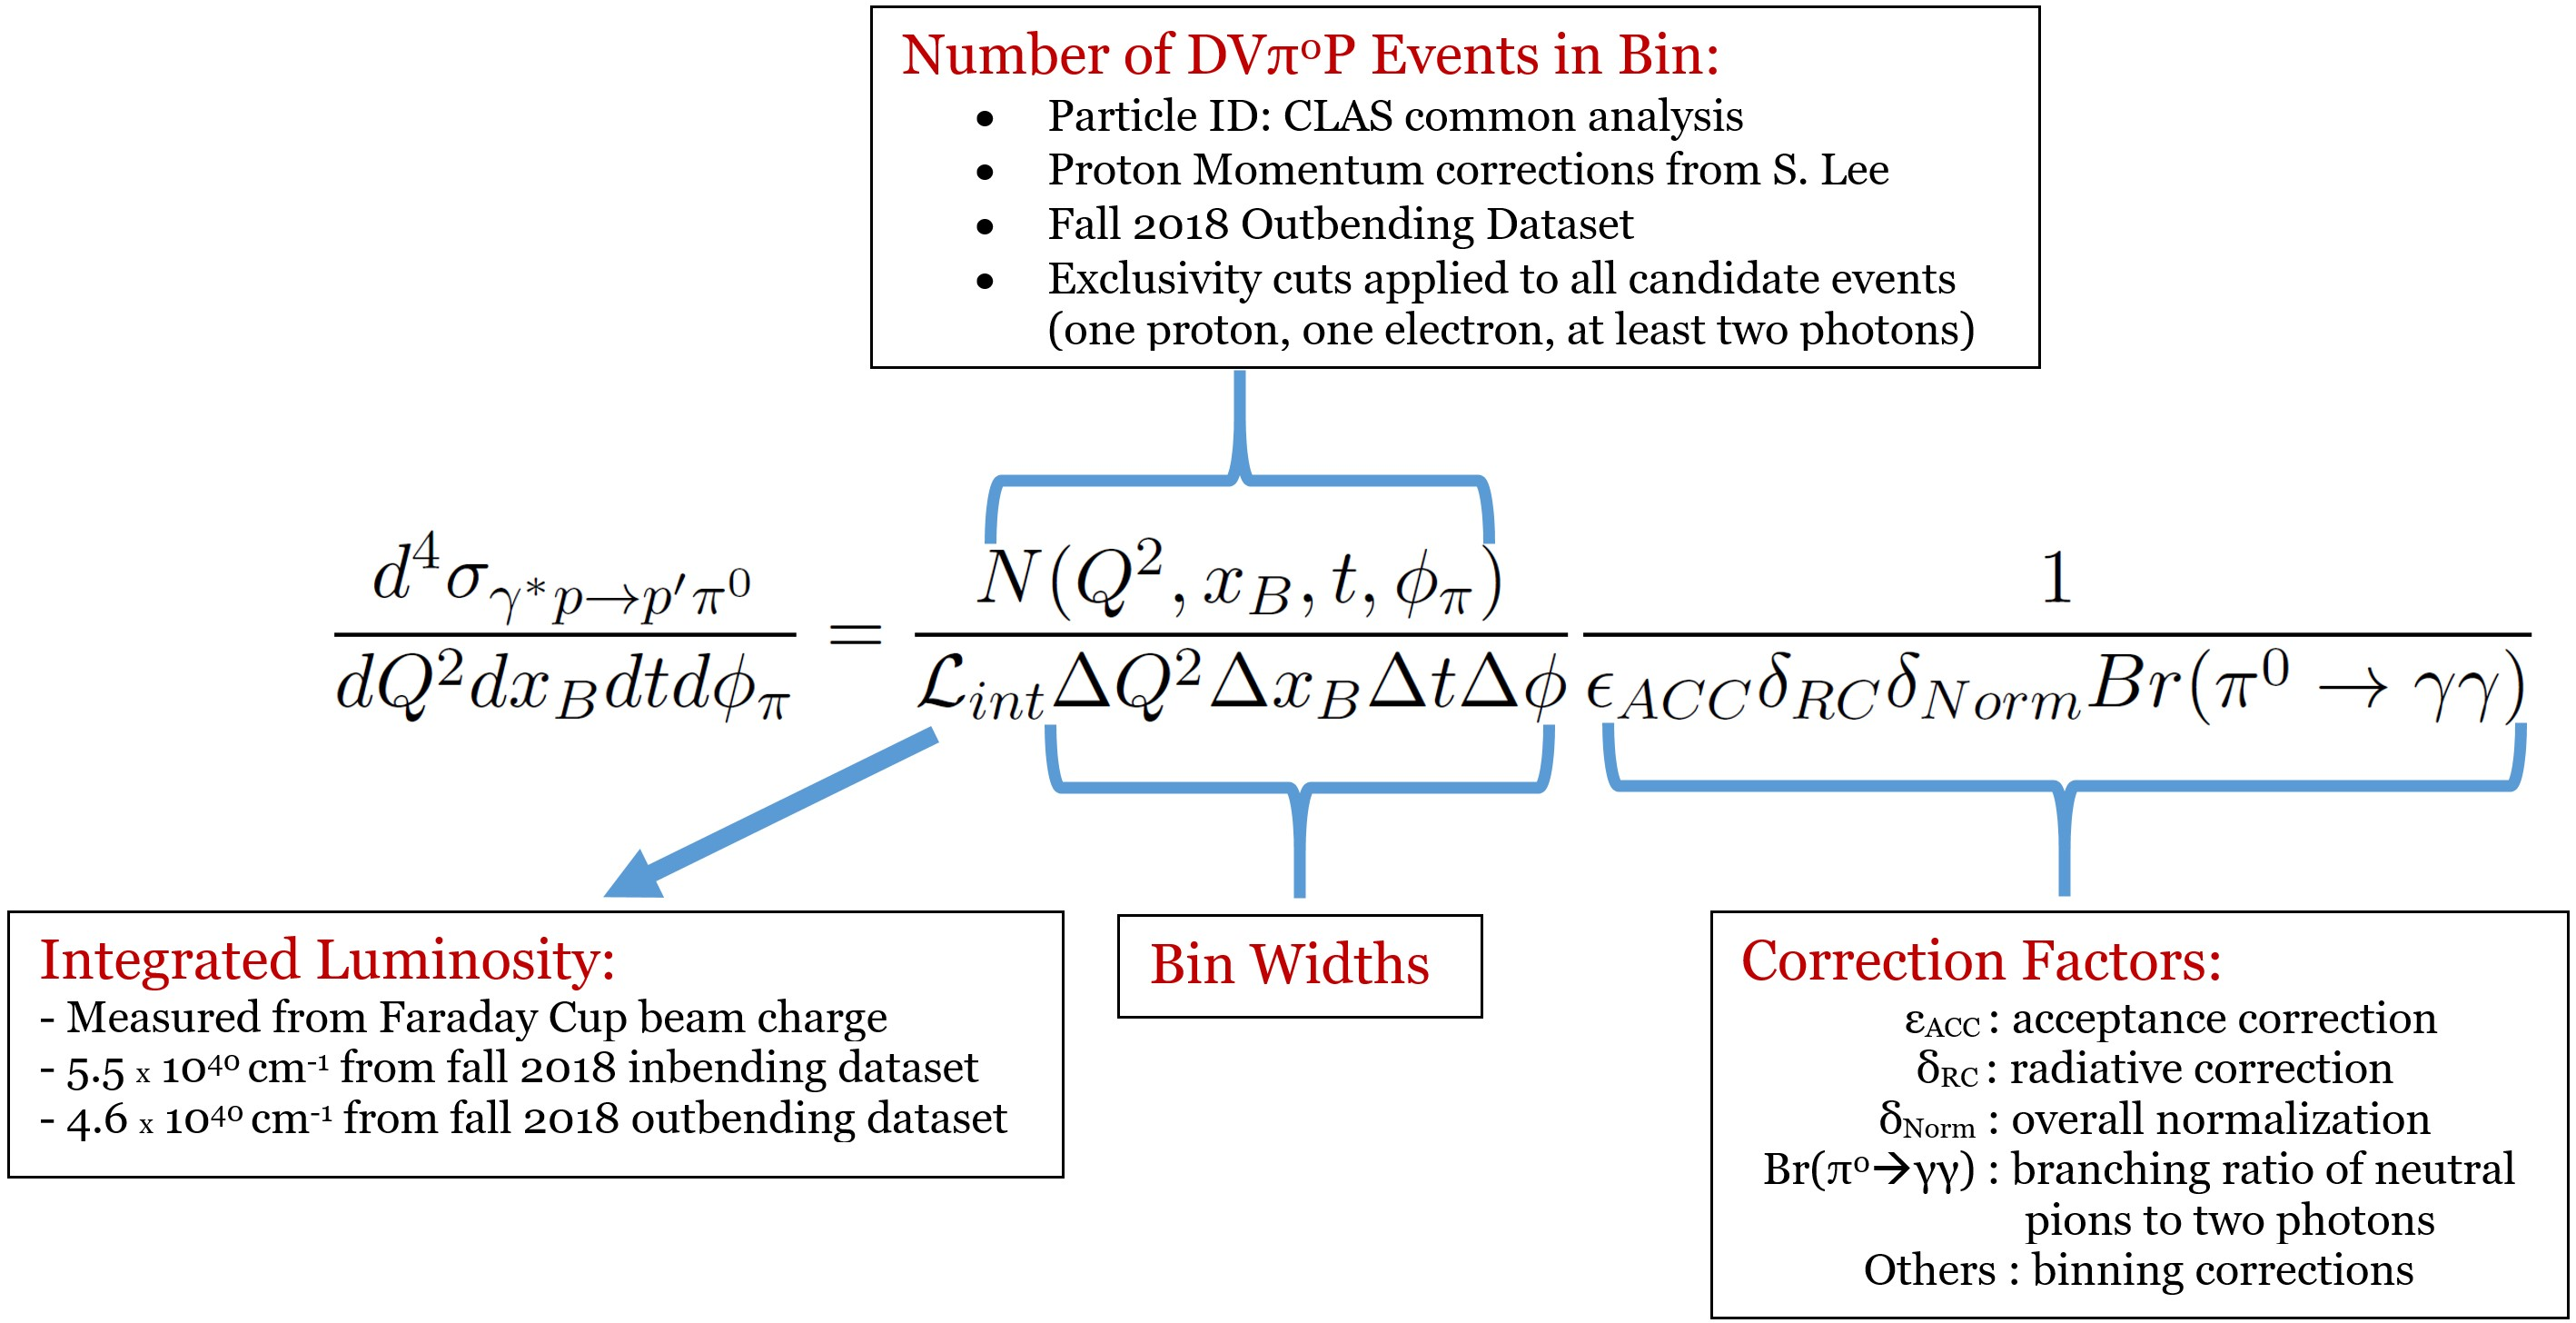
\includegraphics[trim={0 0  0 0cm} ,clip,width=.791725995\textwidth]{extra/steps3.jpg}};
            % The overlayed rectangle
            \fill[blue, opacity=0.25] (4.2cm,2.75cm) rectangle (4.85cm,3.15cm);
        \end{tikzpicture}
    \end{figure}
\end{frame}

\begin{frame}{Components of Cross Section: Event Counts}


    \begin{figure}[h]
        \centering
        \begin{tikzpicture}
            \node[anchor=south west,inner sep=0] at (0,0) {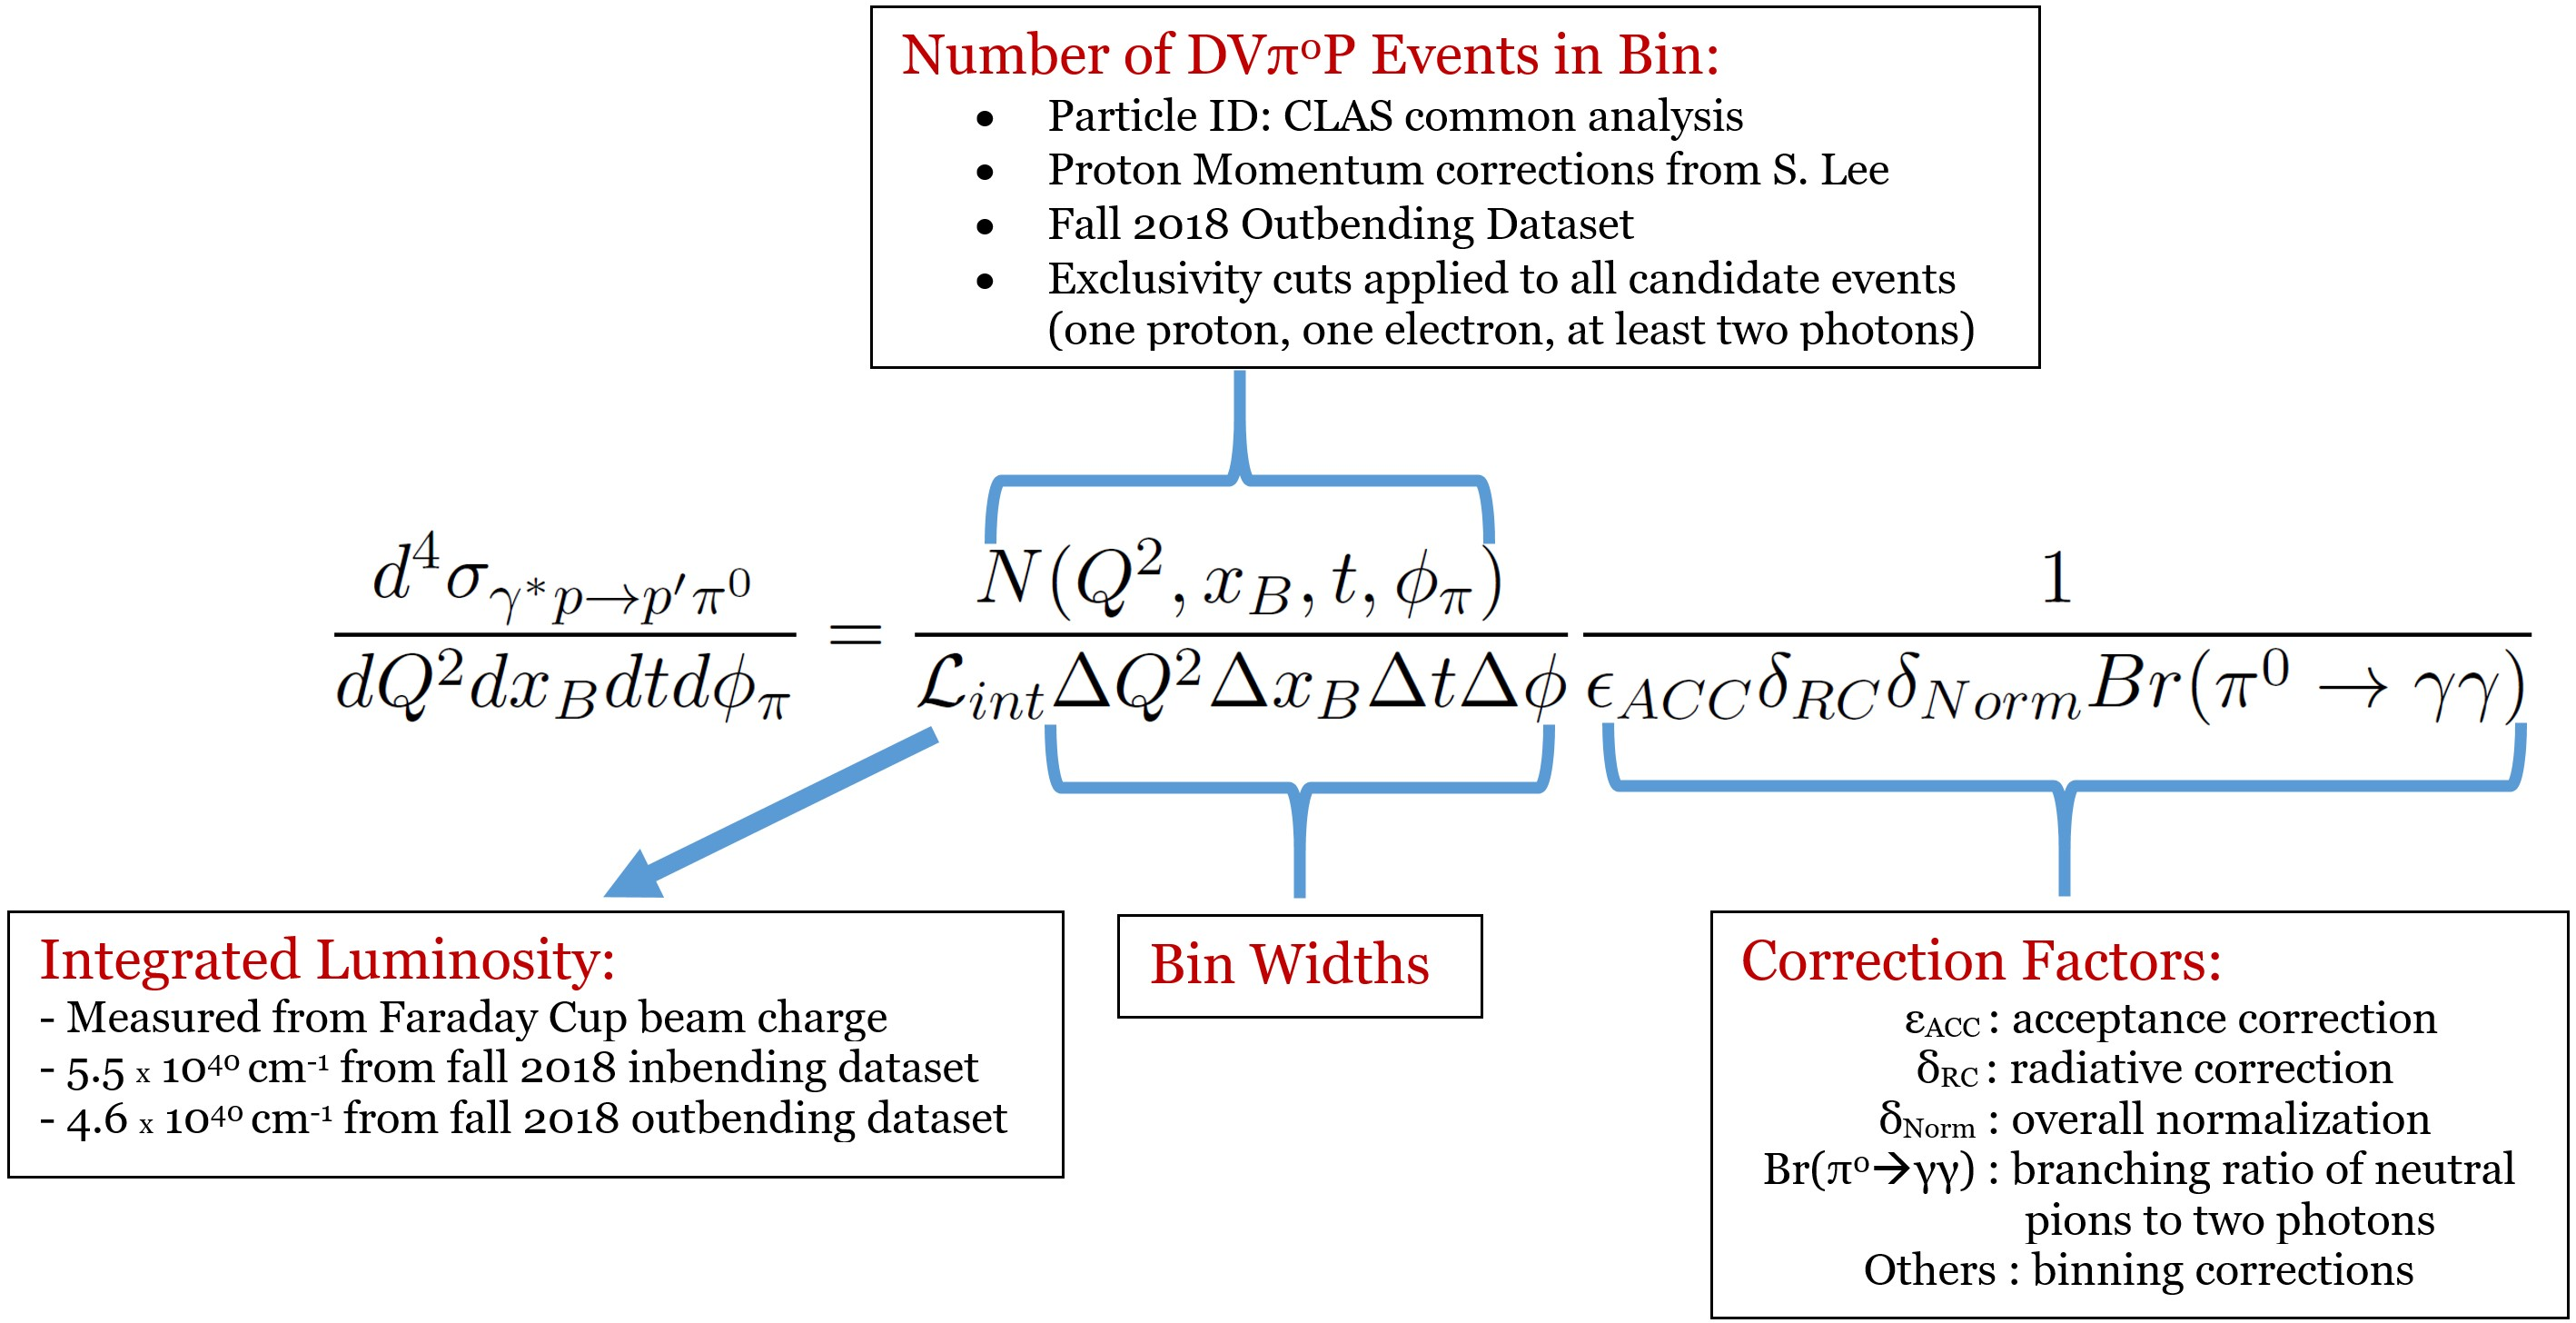
\includegraphics[trim={0 0  0 0cm} ,clip,width=.791725995\textwidth]{extra/steps3.jpg}};
            % The overlayed rectangle
            \fill[blue, opacity=0.25] (4.2cm,2.75cm) rectangle (4.85cm,3.15cm);
            \fill[green, opacity=0.25] (4.5cm,3.25cm) rectangle (7cm,3.65cm);
        \end{tikzpicture}
    \end{figure}
\end{frame}


\begin{frame}{Events and Preliminary Particle Identification} \label{frame:datasets2}
        \vspace{-0.5cm}
        \begin{columns}[t, onlytextwidth]
            \column{0.5\textwidth}
                %\vspace{1cm}
                \begin{figure}[t!]
                    %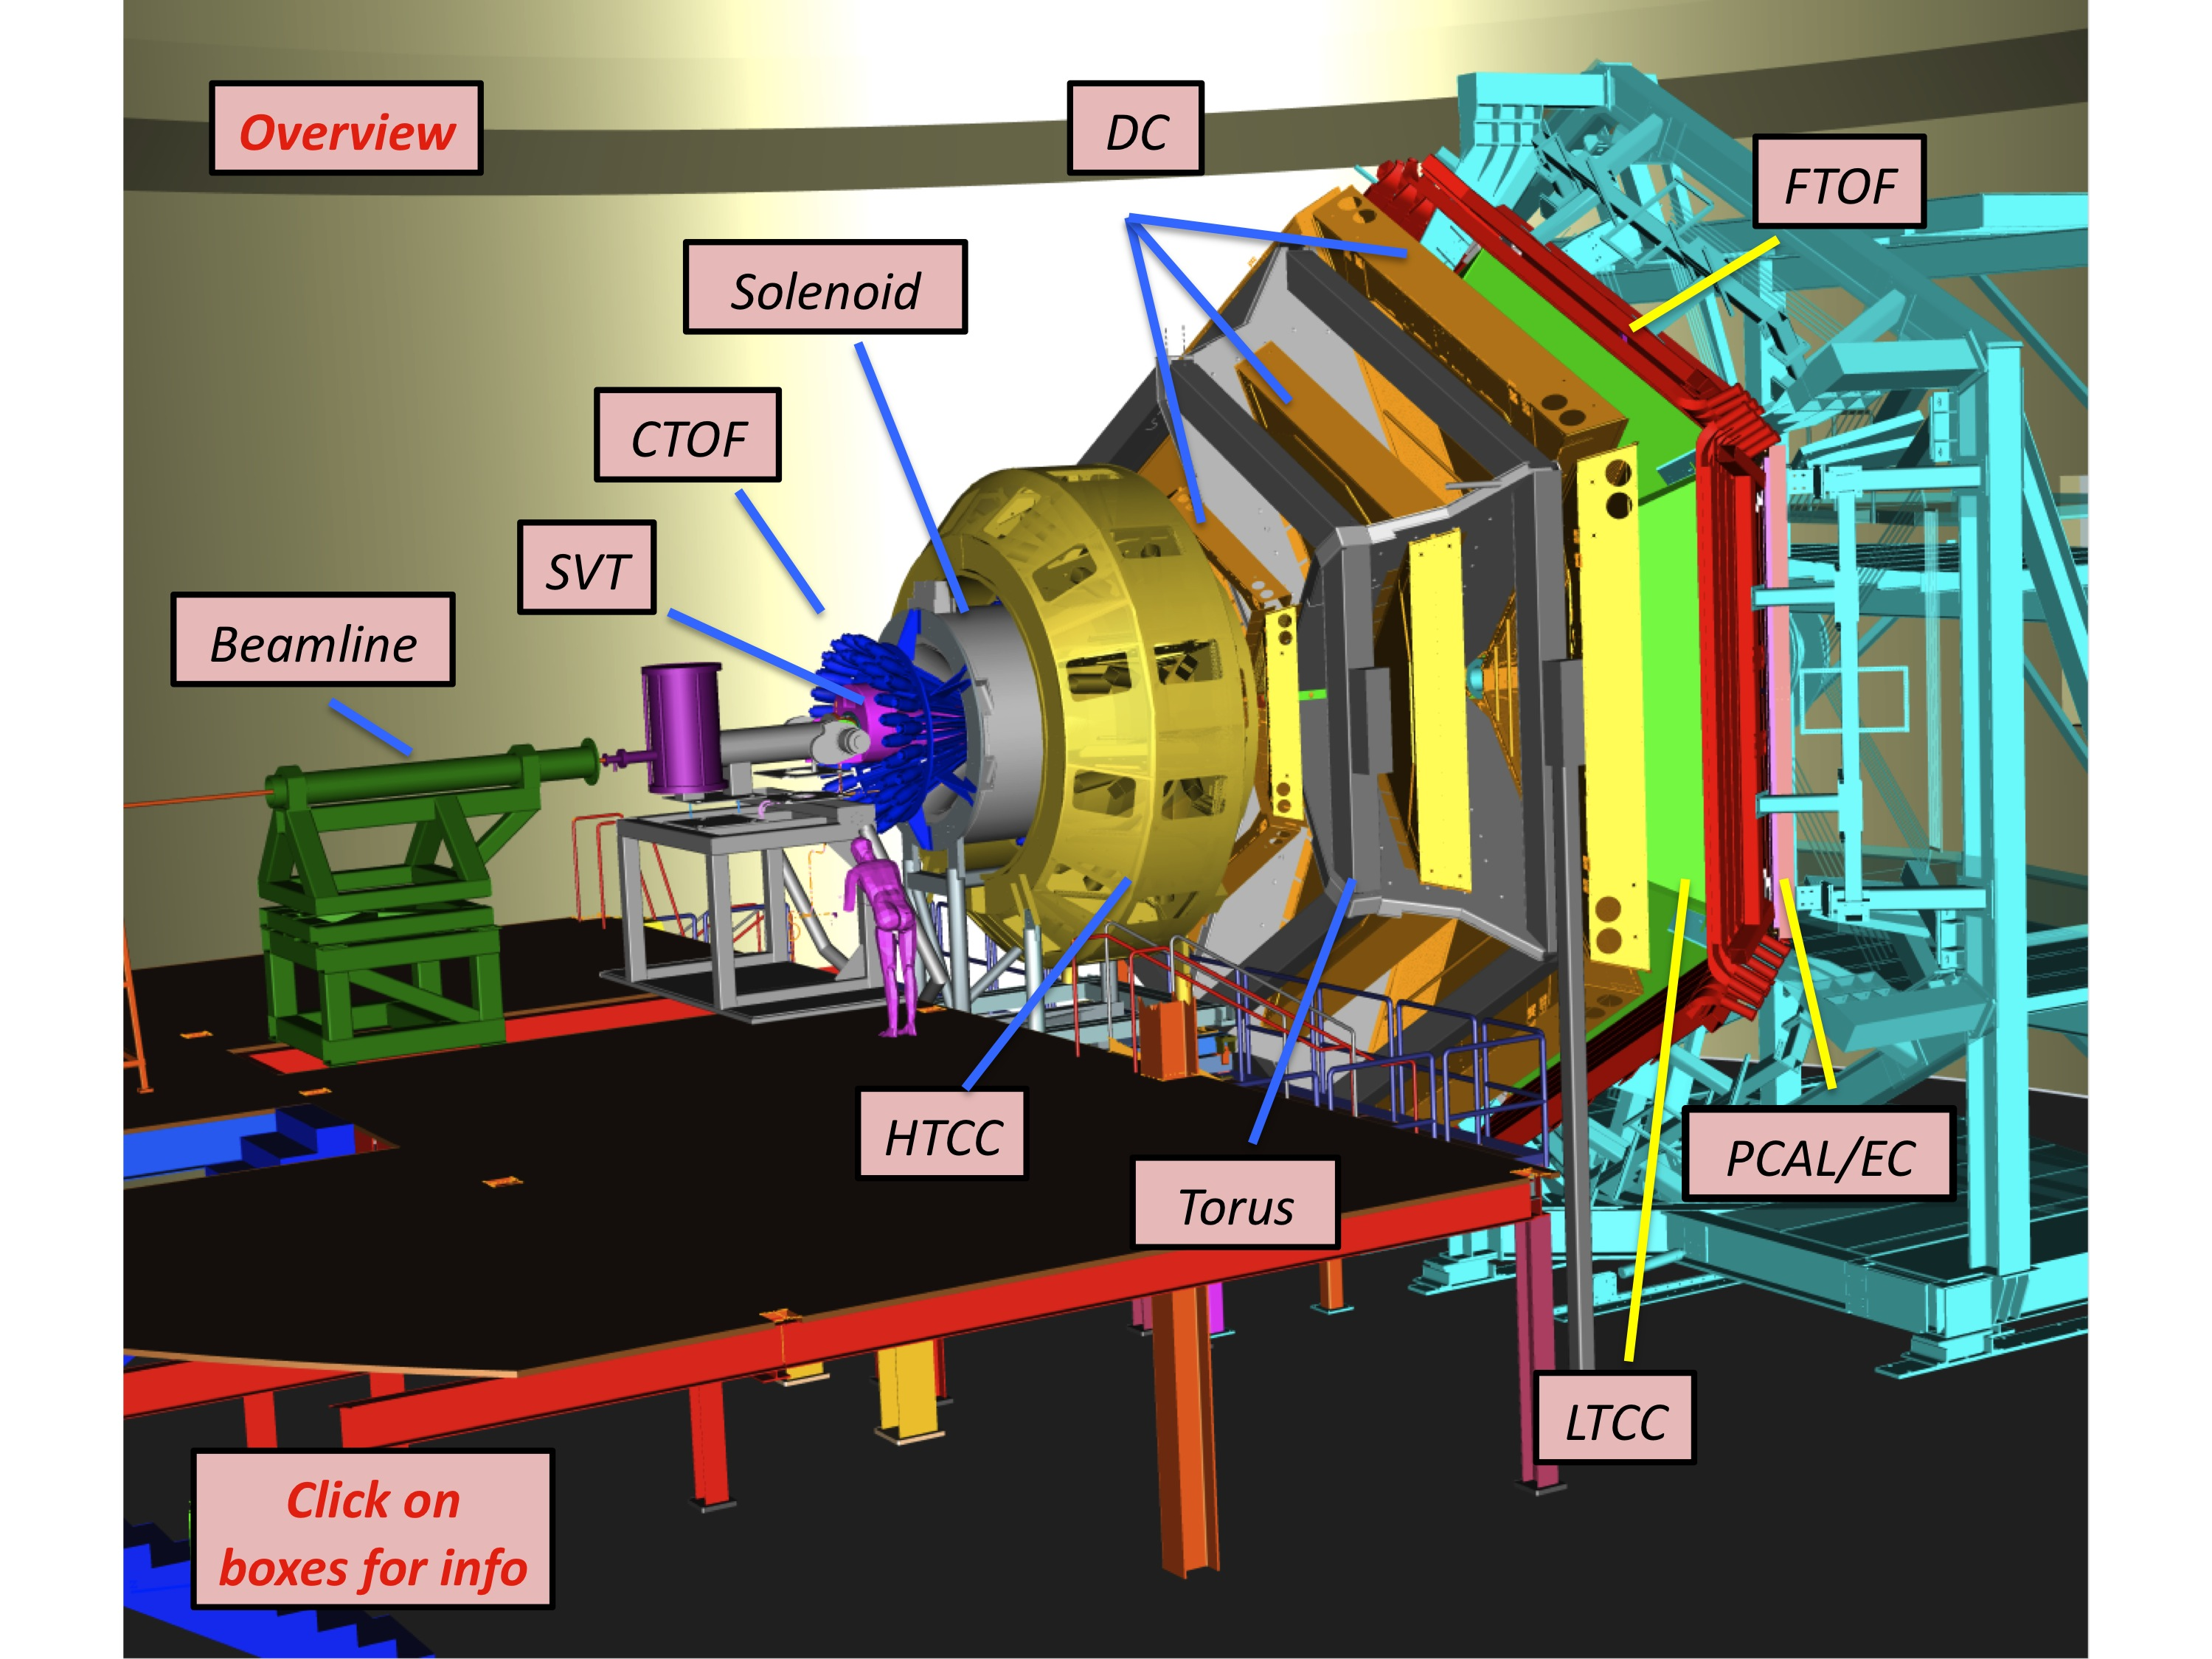
\includegraphics[height=\dimexpr0.5\textheight-0.5in]{Pics/dnp/clas12-overview.jpg}
                    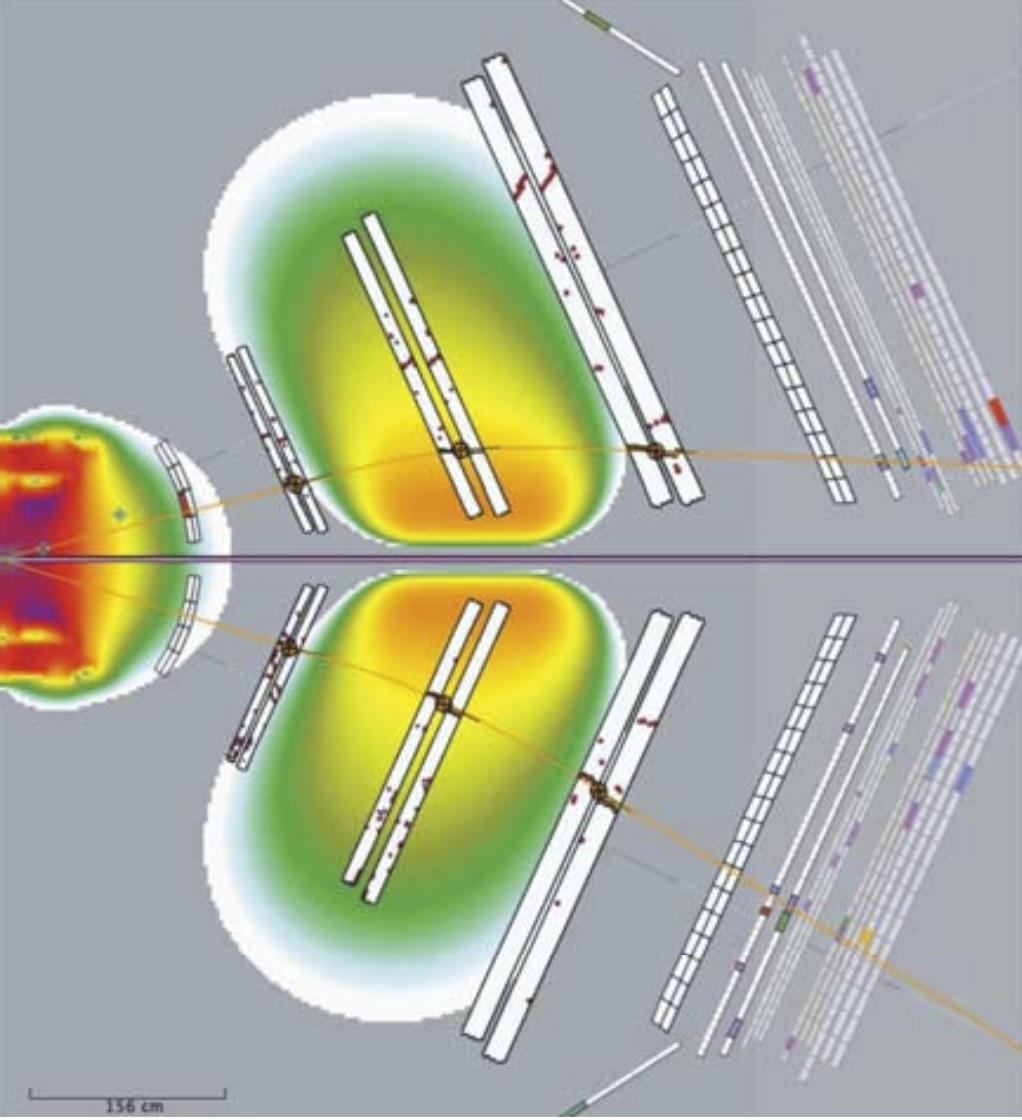
\includegraphics[width=.76349\textwidth]{midana/example_event.png}
                    \caption{ Sample Recon. Event with Detector Hits}
                    
                \end{figure}
                \vspace{-0.45cm}
                
                    
            \column{0.5\textwidth}
                \begin{itemize}
                    \item Reconstruction conducted at collaboration level
                    \item Provides particle features (momentum, charge, mass)
                    \item Additional fiducial cuts, momentum corrections applied afterwards
                \end{itemize}
   \begin{columns}[t, onlytextwidth]
            \column{0.5\textwidth}
             \begin{figure}[t!]
                    %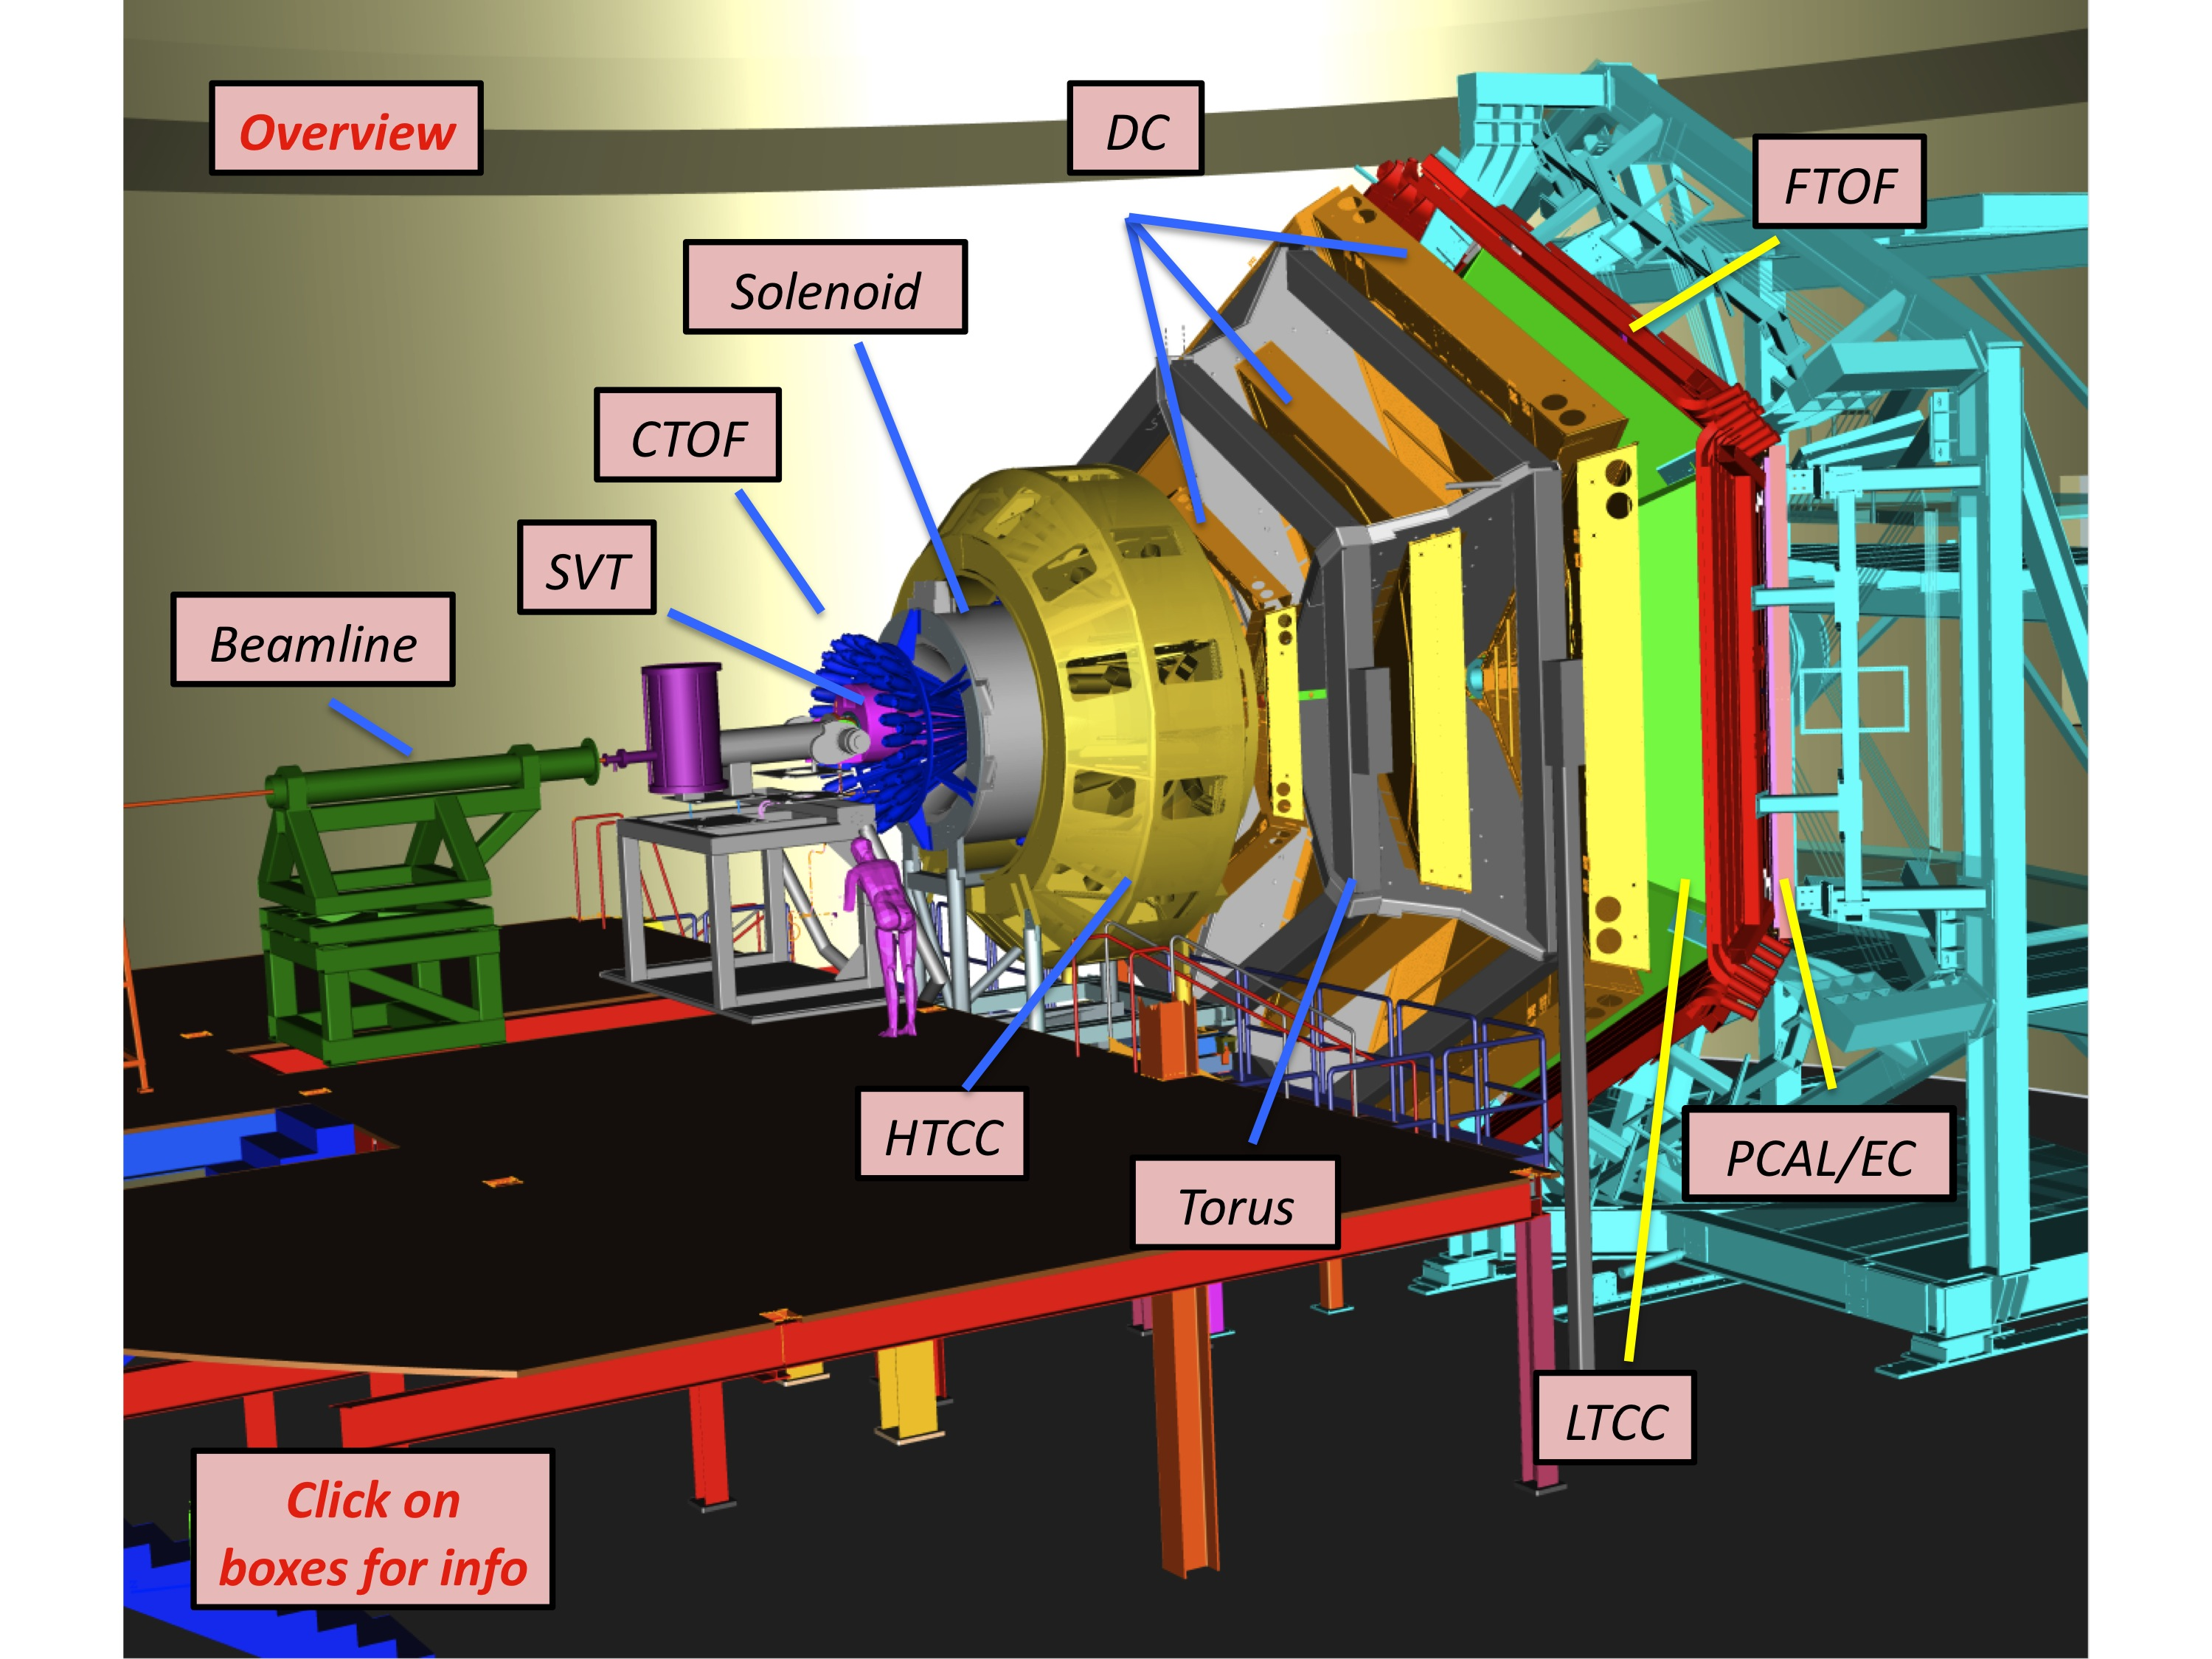
\includegraphics[height=\dimexpr0.5\textheight-0.5in]{Pics/dnp/clas12-overview.jpg}
                    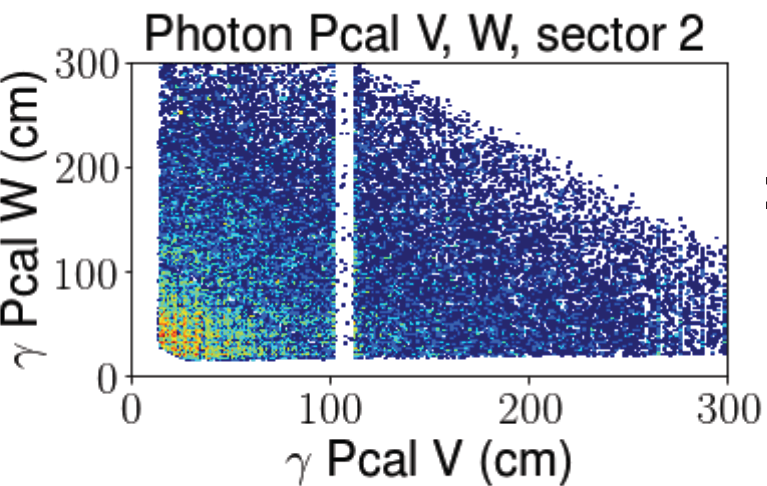
\includegraphics[trim={0 0  0 0cm} ,clip,width=.92\textwidth]{midana/pcalcut.png}
                    
                    
                    
                \end{figure}
            \column{0.5\textwidth}
            
                    \begin{figure}[t!]
                    %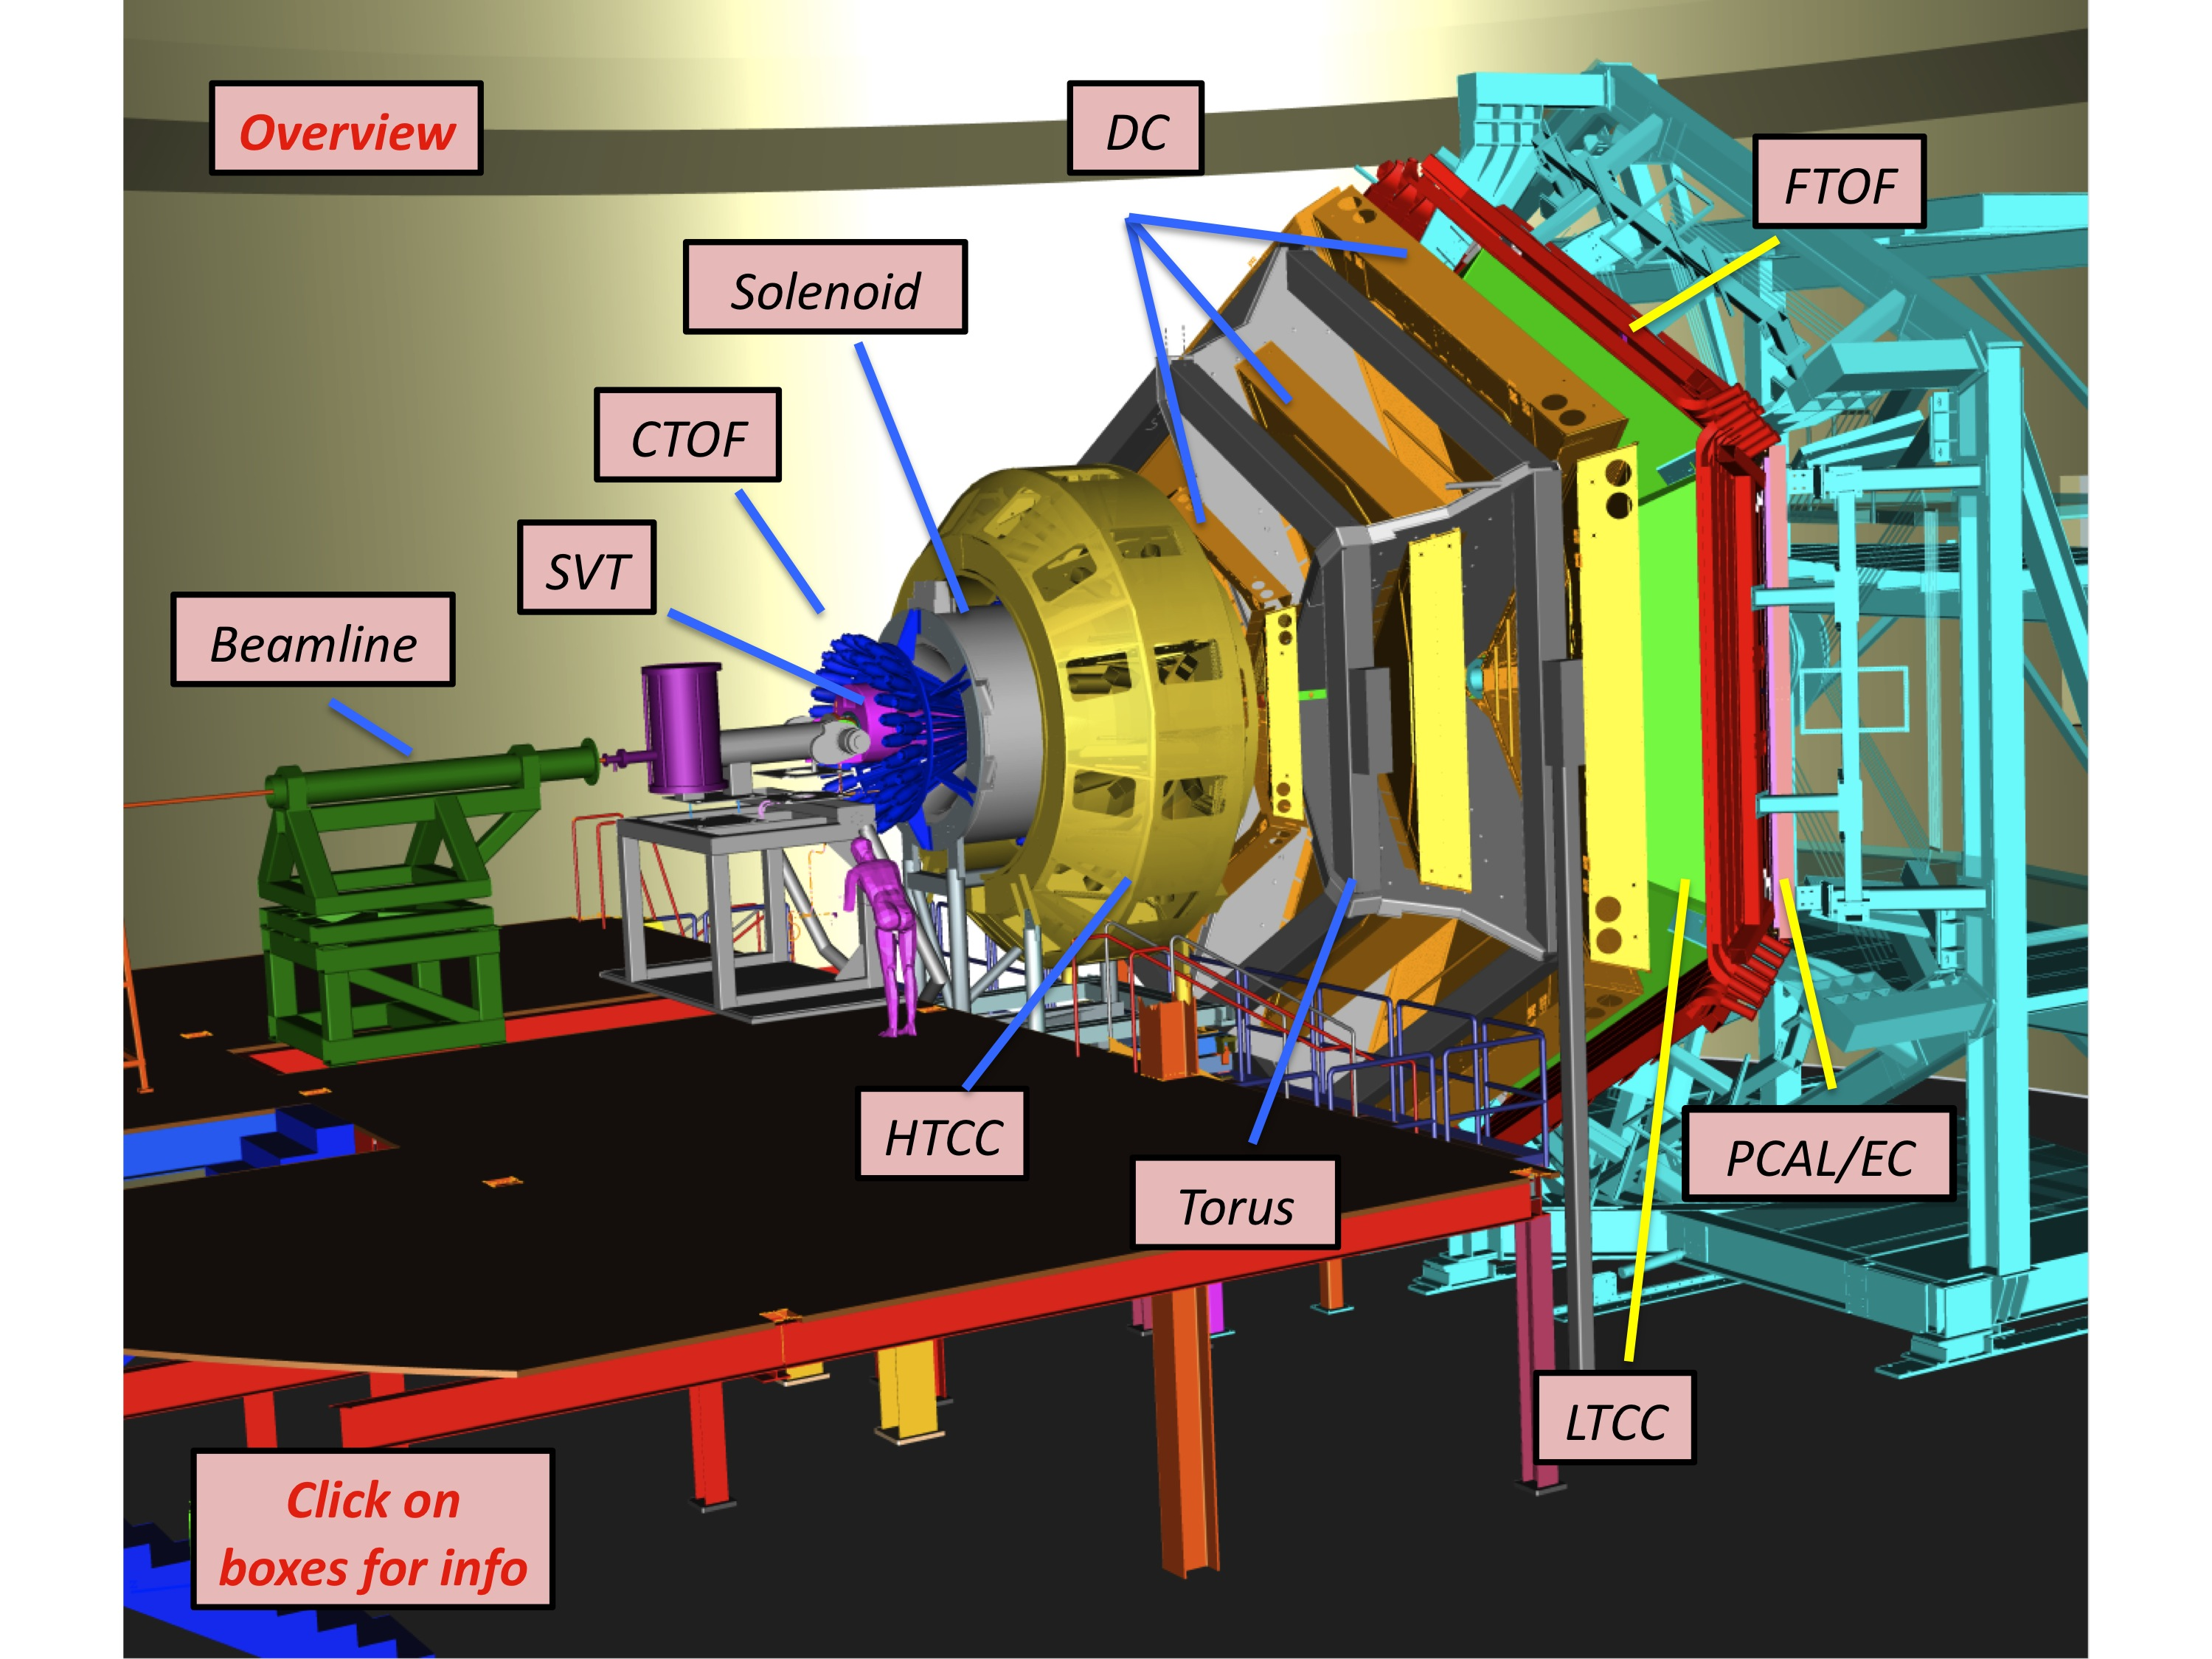
\includegraphics[height=\dimexpr0.5\textheight-0.5in]{Pics/dnp/clas12-overview.jpg}
                    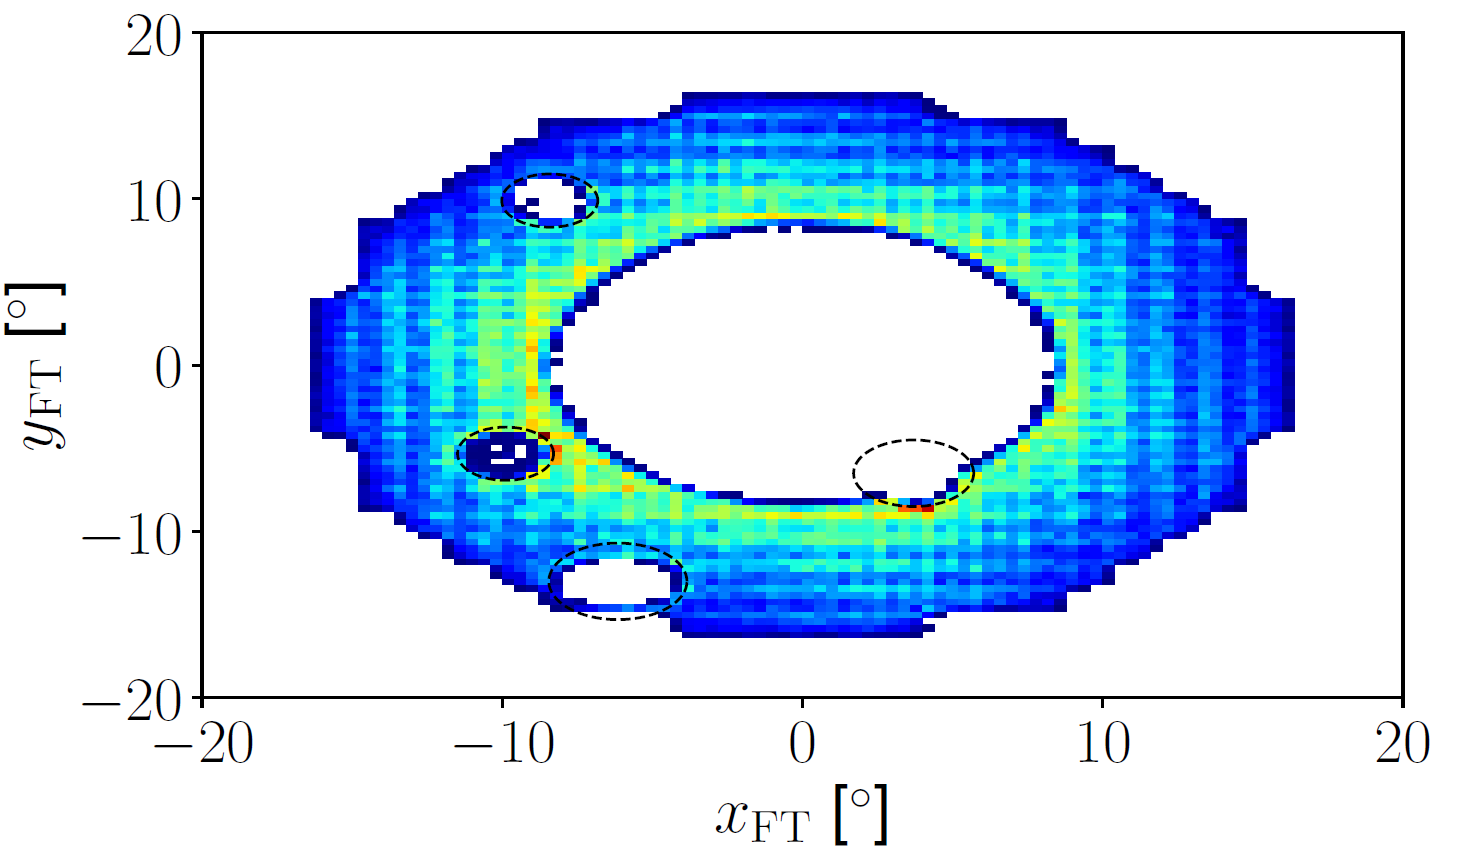
\includegraphics[width=.958565899\textwidth]{midana/fiducial_cuts.png}
                    
                    
                    
                             \end{figure}
               
              
                %Additional fiducial cuts
                %\vspace{0.3cm}
                %{\myfont{\tiny [V. Burkert et al., NIMA, 959, 163419 (2020)] }}
        \end{columns}
          %\vspace{-0.45cm}
          \centering
        {\myfont{\tiny [S. Lee] }}

        \end{columns}
\end{frame}    

%\begin{frame}{Event note}
%Fix CLAS12 slide to show better how particles are found like how Sangbaek did it and include specs (e.g. resolution of 3.3 sigma up to 5 GeV from NIMA paper)
%\end{frame}

\begin{frame}{Event Selection - Particle Identification and Exclusivity Cuts}

        
        \begin{columns}[c]
           \begin{column}{0.35\textwidth}
            \centering \textbf{\underline{Particle Kinematics}}
                %\vspace{1cm}
                \begin{itemize}
                    \item Electron
                        \begin{itemize}
                            \item Cherenkov Counter (PID)
                            \item Drift Chamber (momentum)
                            \item Time-of-flight (PID)
                            \item EM Calorimeter (energy)
                        \end{itemize}
                    \item Proton
                        \begin{itemize}
                            \item Time-of-flights (PID)
                            \item Micromegas, SVT, DCs (momentum)
                        \end{itemize}
                    \item Neutral Pion
                        \begin{itemize}
                            \item EM Calorimeter ($\gamma_1, \gamma_2$)
                            \item $ |M_{\pi^0} - M_{\gamma\gamma}| <$ 40 MeV
                        \end{itemize}
                \end{itemize}
                \end{column}
           %\hspace{-50pt}
            \vrule{}
            \begin{column}{0.65\textwidth}
            
            \centering  \textbf{\underline{Event Cuts}}
                    \begin{columns}[t, onlytextwidth]
            \column{0.45\textwidth}
                
                \begin{itemize}
                 \setlength\itemsep{0.5em}
                \item DIS Cuts
                   
                     \begin{itemize}
                     \setlength\itemsep{0.5em}
        
                    	\item  $Q^2 >$ 1 GeV$^2$
                    	\item W$^2 >$ 4 GeV$^2$
                		\end{itemize}
                		
                	\item Exclusivity Cuts
                	 \begin{itemize}
                     \setlength\itemsep{0.5em}	
                	\item $MM^2_{epX}<0.7$ GeV$^2$
                	
                	\item $M E_{ep \gamma \gamma}<0.7$ GeV

                	
                	\item $\theta_{X\pi}<2^\circ$
                	                	
                	\item $\Delta p_{x,y} <0.3$ GeV
                	\end{itemize}
                	\end{itemize}

        \column{0.55\textwidth}
                    %\textcolor{white}{blank space}

                
                        %#---------------------------------------------
                       	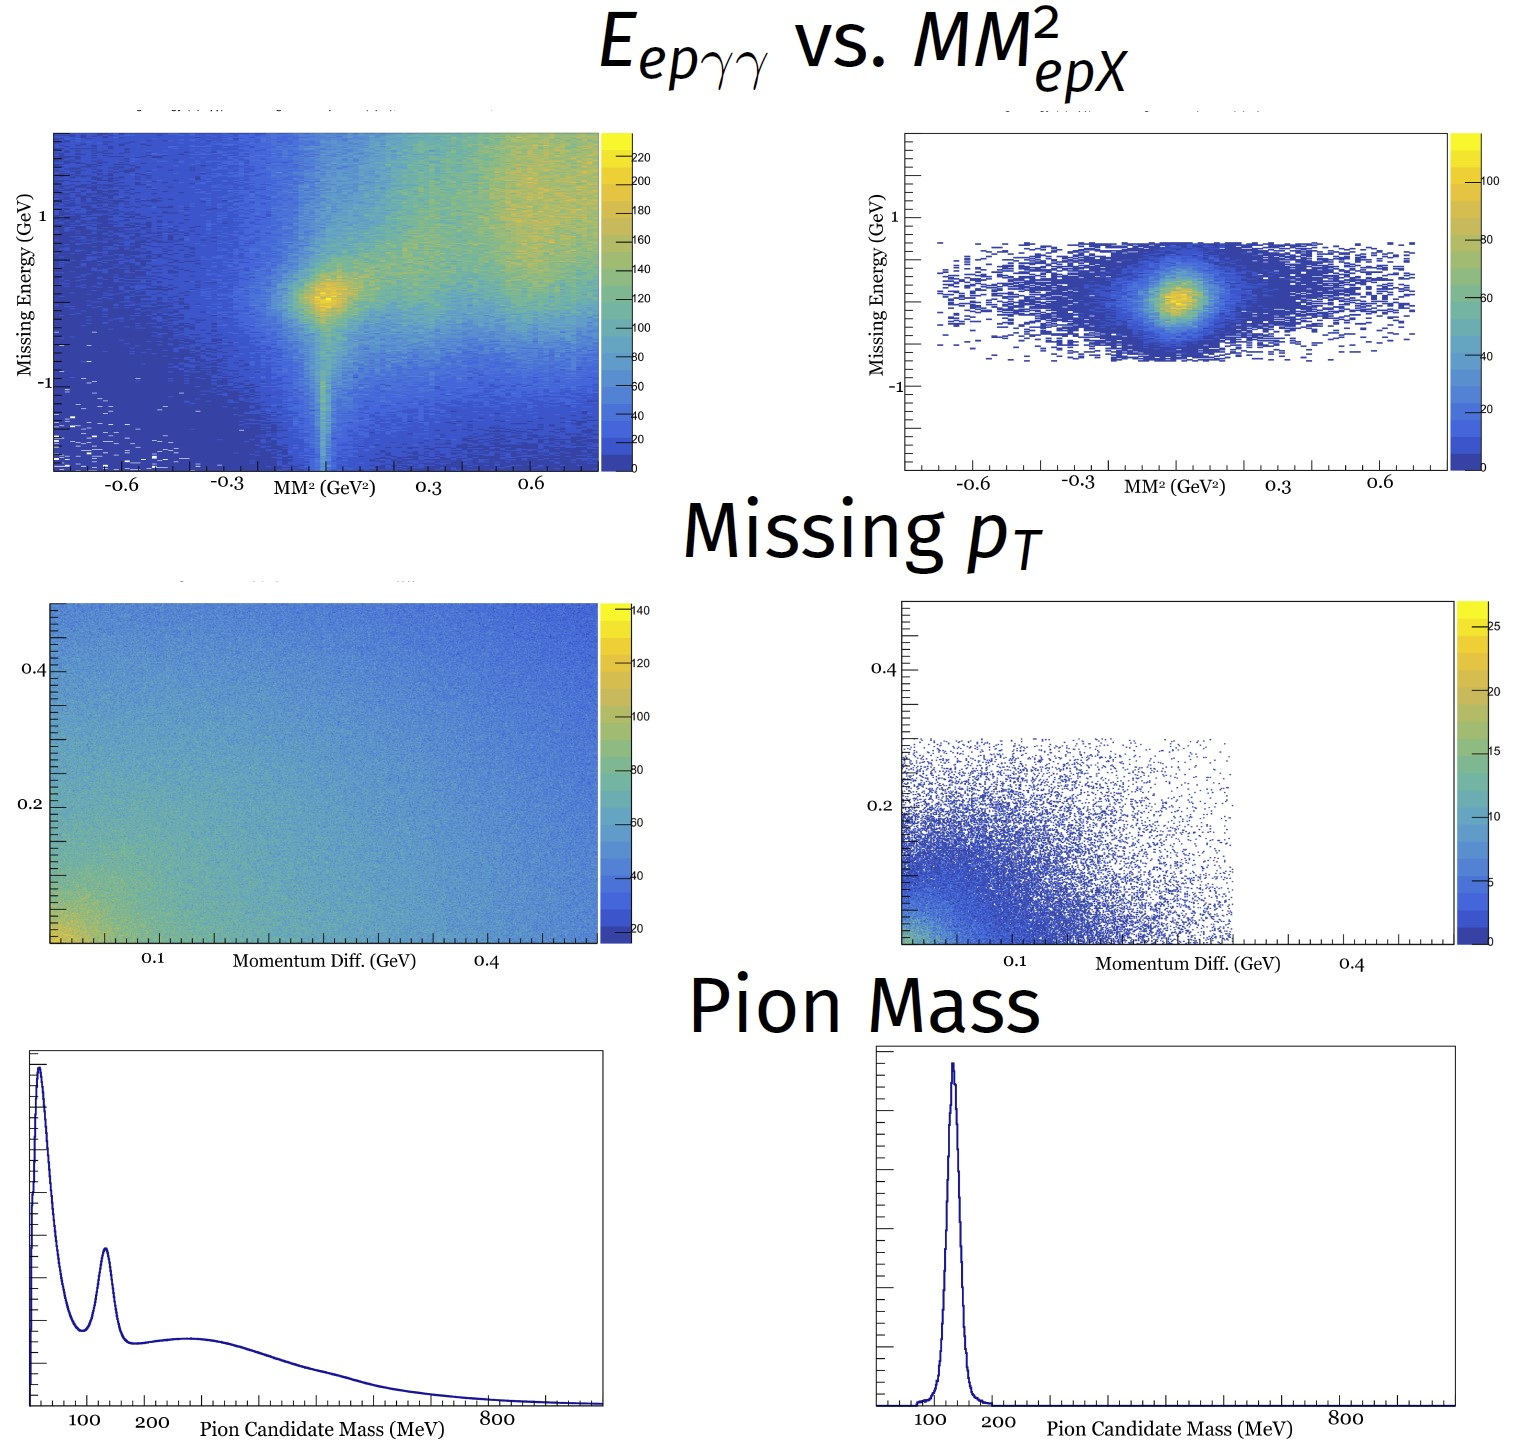
\includegraphics[trim={0 0  0 0cm} ,clip,width=.92\textwidth]{extra/exclusivity.jpg}

                	


        \end{columns}
        \end{column}   
        \end{columns}
\end{frame}

\begin{frame}{Data Pipeline}

        
        \begin{columns}
                                
    
            \column{0.5\textwidth}
                \begin{figure}
                    \centering
                    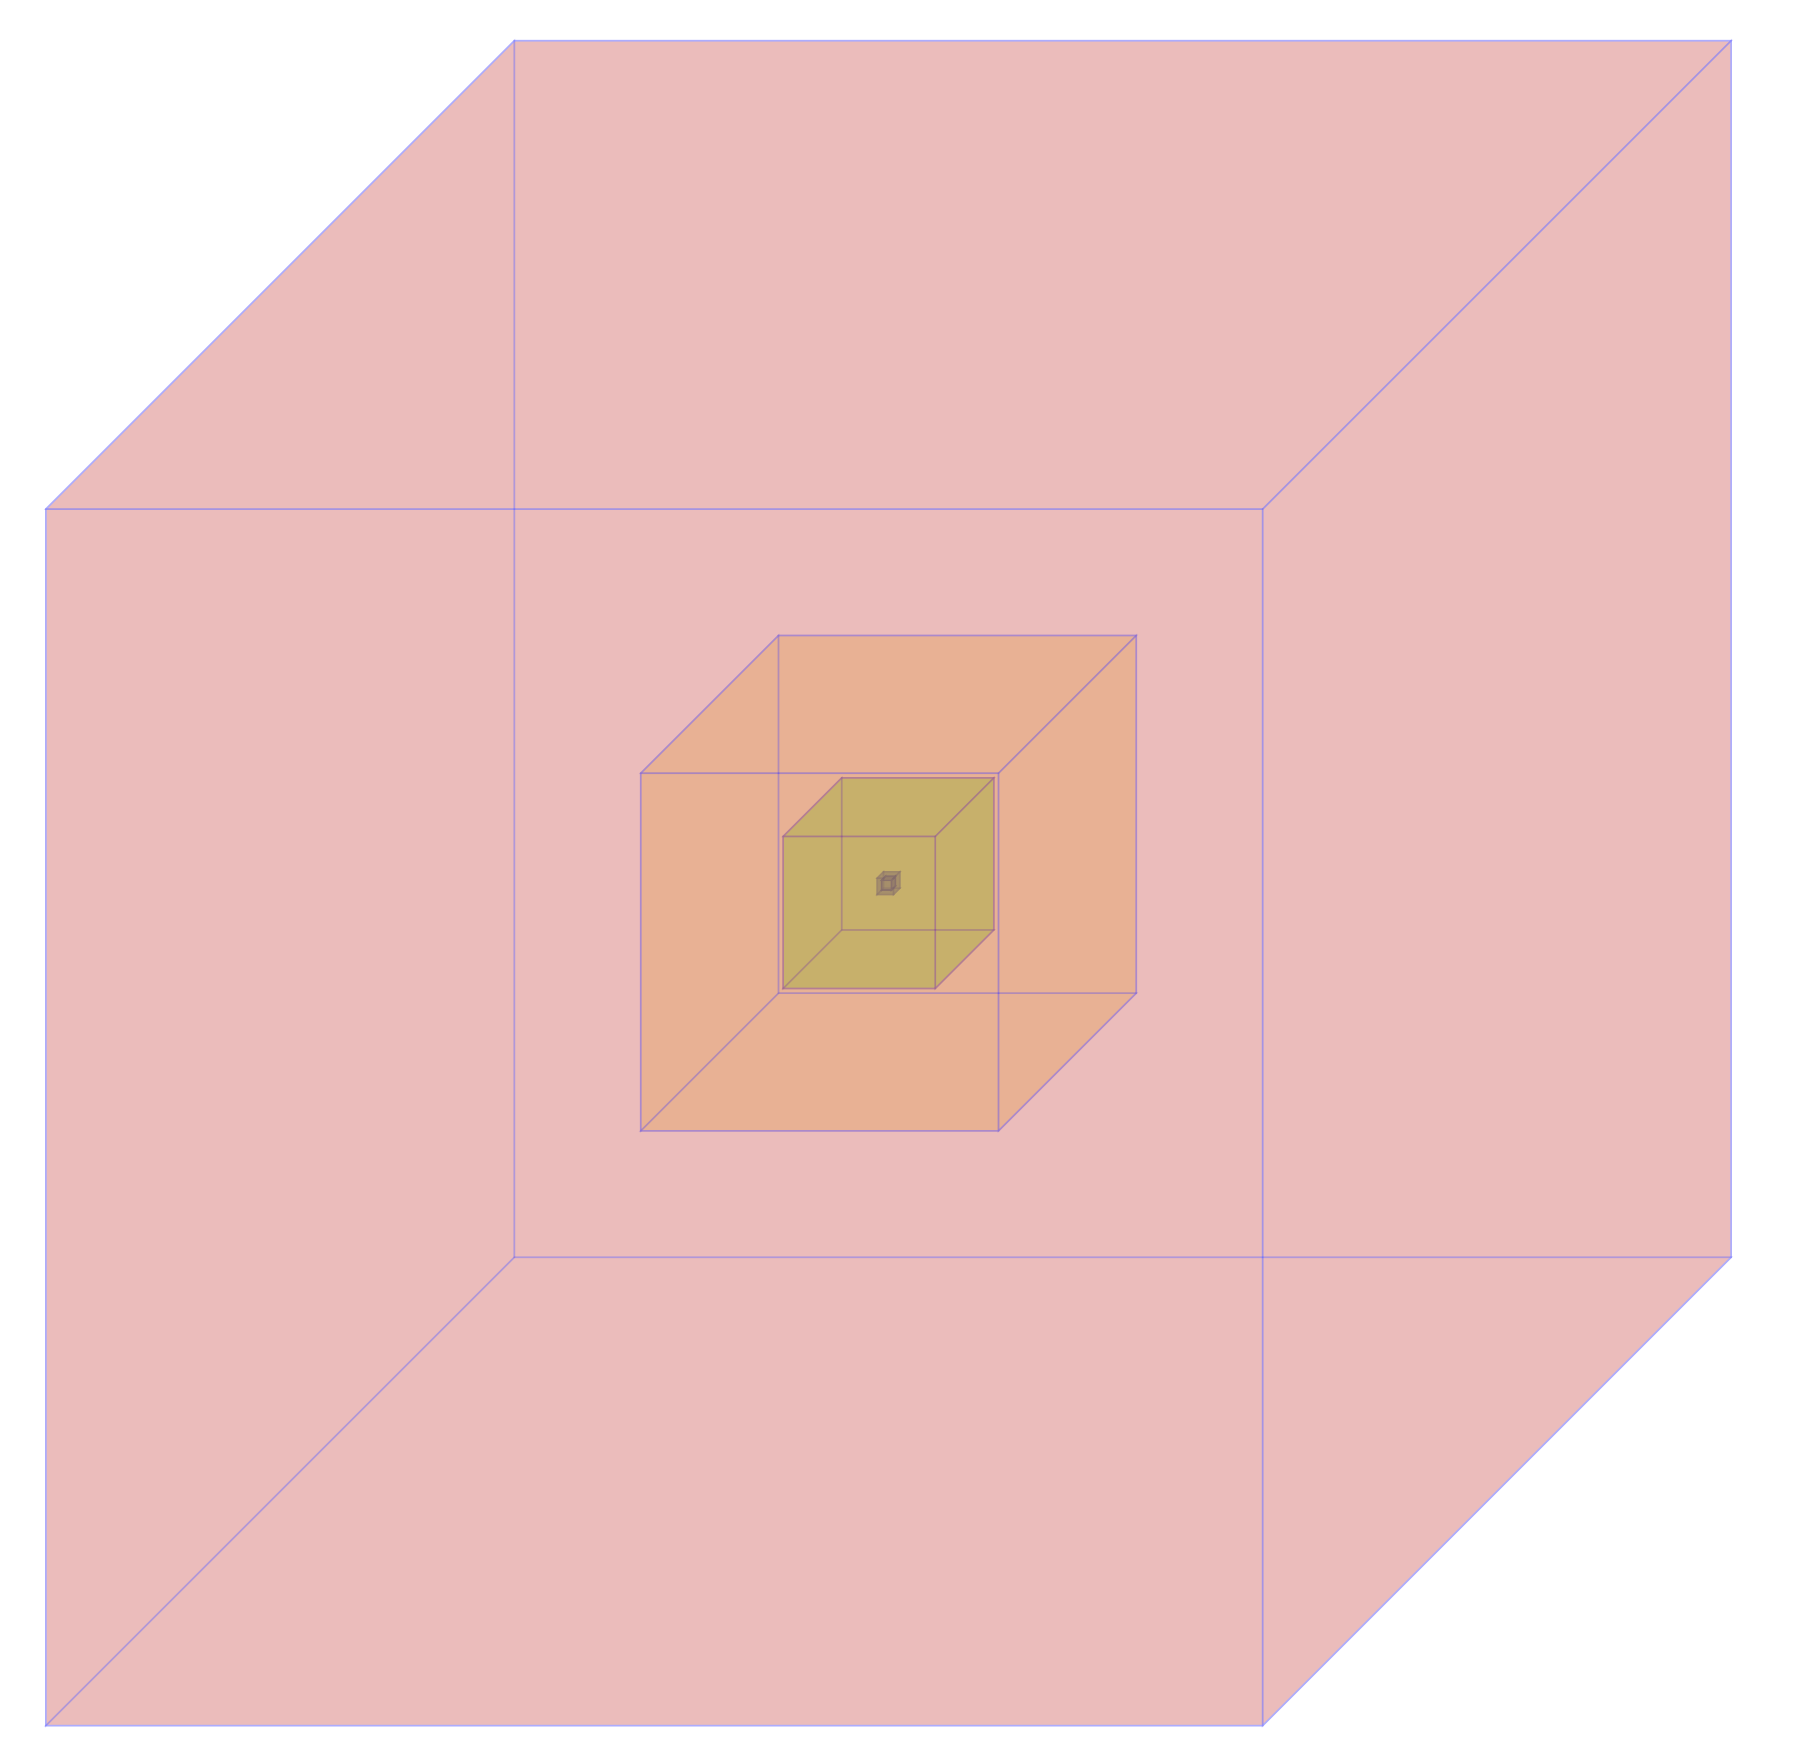
\includegraphics[width=0.6\textwidth]{defense/box1.png}
                    \caption{Caption}
                    \label{fig:enter-label}
                \end{figure}
                    \column{0.5\textwidth}
                \begin{figure}
                    \centering
                    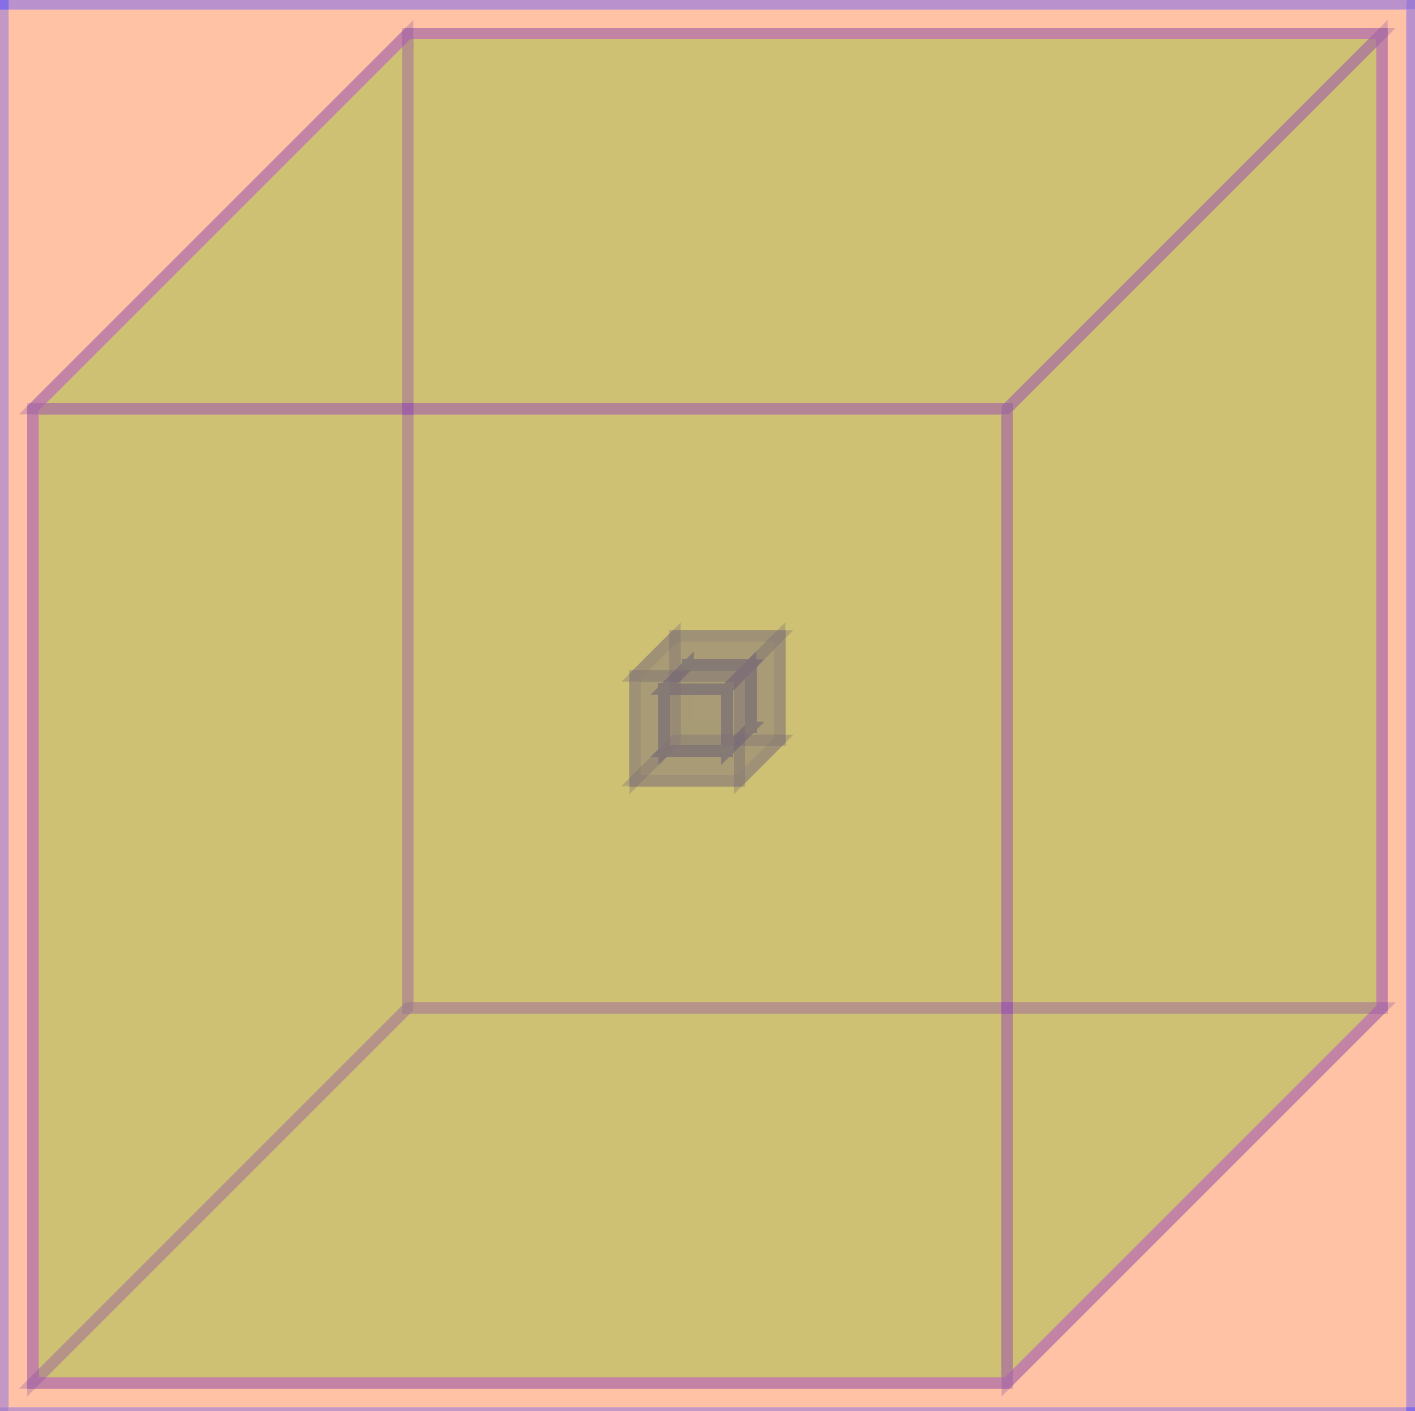
\includegraphics[width=0.6\textwidth]{defense/box2.png}
                    \caption{Caption}
                    \label{fig:enter-label}
                \end{figure}
                
        \end{columns}
       Calculated Integrated Luminosity from Fall 2018  dataset: 5.512 e+40 $cm^{-2}$ inbending, 4.652 e+40 $cm^{-2}$ outbending
\end{frame} 


\begin{frame}{Components of Cross Section}

    \begin{figure}[h]
        \centering
        \begin{tikzpicture}
            \node[anchor=south west,inner sep=0] at (0,0) {\includegraphics[trim={0 0  0 0cm} ,clip,width=.791725995\textwidth]{extra/steps3.jpg}};
            % The overlayed rectangle
                        \fill[blue, opacity=0.25] (4.2cm,2.75cm) rectangle (4.85cm,3.15cm);
            \fill[blue, opacity=0.25] (4.5cm,3.25cm) rectangle (7cm,3.65cm);
        \end{tikzpicture}
    \end{figure}
\end{frame}

\begin{frame}{Components of (Binned) Cross Section: Bin Width}

    \begin{figure}[h]
        \centering
        \begin{tikzpicture}
            \node[anchor=south west,inner sep=0] at (0,0) {\includegraphics[trim={0 0  0 0cm} ,clip,width=.791725995\textwidth]{extra/steps3.jpg}};
            % The overlayed rectangle
                       \fill[blue, opacity=0.25] (4.2cm,2.75cm) rectangle (4.85cm,3.15cm);
            \fill[blue, opacity=0.25] (4.5cm,3.25cm) rectangle (7cm,3.65cm);
            \fill[green, opacity=0.25] (4.85cm,2.75cm) rectangle (7.28cm,3.15cm);
        \end{tikzpicture}
    \end{figure}
\end{frame}

\begin{frame}{Event Binning}

\begin{columns}
        \column{0.3\textwidth}
        words about binning
        \column{0.35\textwidth}    
            \begin{figure}
                \centering
                \includegraphics[width=0.97\textwidth]{defense/x_B_vs_Q2,_Exp_Inbend.png}
                \caption{Caption}
                \label{fig:enter-label}
            \end{figure}
                    \column{0.35\textwidth}    
            \begin{figure}
                \centering
                \includegraphics[width=0.97\textwidth]{defense/phi_vs_Momentum_Transfer_t,_Exp_Inbend.png}
                \caption{Caption}
                \label{fig:enter-label}
            \end{figure}

\end{columns}
\end{frame}


\begin{frame}{Components of Cross Section}

    
    \begin{figure}[h]
        \centering
        \begin{tikzpicture}
            \node[anchor=south west,inner sep=0] at (0,0) {\includegraphics[trim={0 0  0 0cm} ,clip,width=.791725995\textwidth]{extra/steps3.jpg}};
            % The overlayed rectangle
            \fill[blue, opacity=0.25] (4.2cm,2.75cm) rectangle (4.85cm,3.15cm);
            \fill[blue, opacity=0.25] (4.5cm,3.25cm) rectangle (7cm,3.65cm);
            \fill[blue, opacity=0.25] (4.85cm,2.75cm) rectangle (7.28cm,3.15cm);
        \end{tikzpicture}
    \end{figure}
\end{frame}


\begin{frame}{Components of Cross Section: Correction Factors}

    
    \begin{figure}[h]
        \centering
        \begin{tikzpicture}
            \node[anchor=south west,inner sep=0] at (0,0) {\includegraphics[trim={0 0  0 0cm} ,clip,width=.791725995\textwidth]{extra/steps3.jpg}};
            % The overlayed rectangle
            \fill[blue, opacity=0.25] (4.2cm,2.75cm) rectangle (4.85cm,3.15cm);
            \fill[blue, opacity=0.25] (4.5cm,3.25cm) rectangle (7cm,3.65cm);
            \fill[blue, opacity=0.25] (4.85cm,2.75cm) rectangle (7.28cm,3.15cm);
            \fill[green, opacity=0.25] (7.28cm,2.75cm) rectangle (11.68cm,3.15cm);
        \end{tikzpicture}
    \end{figure}
\end{frame}

\begin{frame}{Simulations Needed to Determine Correction Factors}
                  \begin{itemize}
                        \item   High computational demands: 5 hours to simulate 10K events
    \item Need $\mathcal{O}(2B)$ events $\rightarrow$ need 1M core-hours for this analysis alone
    \item Built service to connect research collaboration with HTC nodes worldwide

                    \end{itemize}

    \begin{columns}
            \column{0.2\textwidth}    
            \centering
                    %\vspace{1cm}
                    \includegraphics[trim={0 0  0 0cm} ,clip,width=.8982\textwidth]{sims/osg_logo.png}
                                          
                           \includegraphics[trim={4.1cm 0  0 0cm} ,clip,width=.982\textwidth]{sims/htcondor.png}
            \column{0.4\textwidth} 

    \begin{figure}
                \centering
                \includegraphics[trim={0 0  0 0cm} ,clip,width=.8982\textwidth]{sims/gemc1.png}
                 \end{figure}
            \column{0.4\textwidth}    
            \centering

            \begin{figure}
                \centering
                \includegraphics[trim={0 0  0 0cm} ,clip,width=.8982\textwidth]{sims/gemc2.png}
                \caption{Usage facilitated in 2022}
                \label{fig:my_label}
            \end{figure}                              
                    \end{columns}
  
\end{frame}

\begin{frame}{Event Generator and Simulation Details}
     \begin{columns}[c]
               \begin{column}{0.5\textwidth}

                    %\vspace{1cm}
                    \begin{itemize}
                        \item Event Generator - aao\_(no)rad
                            \begin{itemize}
                                \item  $DVMP$ generator validated on CLAS6 and COMPASS data, origin 1990s
                            \end{itemize}
                        \item Simulation - GEMC
                            \begin{itemize}
                                \item GEANT4 based simulation developed by CLAS collaboration
                            \end{itemize}
                        \item Computing Power
                            \begin{itemize}
                                \item Through OSG pipeline, CLAS has access to supercomputing clusters around the world, including dedicated nodes at MIT Tier 2, UConn, INFN, GRIDPP, new groups still joining
                            \end{itemize}
                    \end{itemize}
                    \end{column}
                    
                    
    \begin{column}{0.5\textwidth}
                
                \centering Generated \\
        \begin{columns}
                    
                    \column{0.5\textwidth}
                        %\textcolor{white}{blank space}
                             
                    
                            %#---------------------------------------------
                           	\includegraphics[trim={0 0  0 0cm} ,clip,width=.982\textwidth]{extra/generator/Lepton-Hadron_Angle_phi_vs_Proton_theta,_Gen.png}
                           	   
                  \column{0.5\textwidth}          	   
                           	
                        	\includegraphics[trim={0 0  0 0cm} ,clip,width=.982\textwidth]{extra/generator/x_B_vs_Q2,_Gen.png}
            
                        \end{columns}
                        \vspace{0.3cm}
              \centering Reconstructed \\      
          \begin{columns} 
            
            
                        \column{0.5\textwidth}
             
                               
                           \includegraphics[trim={0 0  0 0cm} ,clip,width=.982\textwidth]{extra/generator/Lepton-Hadron_Angle_phi_vs_Proton_theta,_rec.png}
           \column{0.5\textwidth}
                              
                        	\includegraphics[trim={0 0  0 0cm} ,clip,width=.982\textwidth]{extra/generator/x_B_vs_Q2,_rec.png}
        
                \end{columns}
    \end{column}
                    
    \end{columns}
\end{frame}


\begin{frame}{Simulation Needs to be Adjusted to Match Experimental Data}


GEANT4 simulation results in reconstructed tracks that are overly optimistic - resolution is better in simulation than in real data



\vspace{0.2cm}
\begin{columns}
            \column{0.32\textwidth}
                %\textcolor{white}{blank space}
                     \centering $ME_{ep\gamma\gamma}$ \\
                        % trim={<left> <lower> <right> <upper>}
                    %#---------------------------------------------
                   	\includegraphics[trim={0 1.75cm  0 3.05cm} ,clip,width=.82\textwidth]{simcomp/nosmear/nosmear_ME_epgg.png}
                   	   \centering  $MM^2_{e\gamma\gamma}$ \\
                	\includegraphics[trim={0 1.75cm  0 3.05cm} ,clip,width=.82\textwidth]{simcomp/nosmear/nosmearMM2_egg.png}


                \column{0.32\textwidth}
     
                       \centering  $MM^2_{ep\gamma\gamma}$ \\
                	\includegraphics[trim={0 1.75cm  0 3.05cm} ,clip,width=.82\textwidth]{simcomp/nosmear/nosmearMM2_epgg.png}
   
                      \centering   $MM^2_{ep}$ \\
                	\includegraphics[trim={0 1.75cm  0 3.05cm} ,clip,width=.82\textwidth]{simcomp/nosmear/nosmearMM2_ep.png}

            
            \column{0.32\textwidth}

                    %#---------------------------------------------
                      \centering   $M_{\gamma\gamma}$ \\
                	\includegraphics[trim={0 1.75cm  0 3.05cm} ,clip,width=.82\textwidth]{simcomp/nosmear/nosmearMpi0.png}
 
                       \centering  $\Delta p_{t}$ \\
                	\includegraphics[trim={0 1.75cm  0 3.05cm} ,clip,width=.82\textwidth]{simcomp/nosmear/nosmearMPt.png}
    \end{columns}
\end{frame} 

\begin{frame}{Smearing Factors makes Simulation More Realistic}

With the addition of smearing factors to simulated particle reconstruction values, the simulation matches experimental distributions well.  {\myfont{\footnotesize [Collaborator S. Lee]}}



\vspace{0.2cm}
\begin{columns}
            \column{0.32\textwidth}
                %\textcolor{white}{blank space}
                     \centering $ME_{ep\gamma\gamma}$ \\
                        % trim={<left> <lower> <right> <upper>}
                    %#---------------------------------------------
                   	\includegraphics[trim={0 1.75cm  0 3.05cm} ,clip,width=.82\textwidth]{simcomp/yessmear/outbending_rad_All_All_All_for_aps_2022_plots_sangcutsME_epgg_exp_vs_sim.png}
                   	   \centering  $MM^2_{e\gamma\gamma}$ \\
                	\includegraphics[trim={0 1.75cm  0 3.05cm} ,clip,width=.82\textwidth]{simcomp/yessmear/outbending_rad_All_All_All_for_aps_2022_plots_sangcutsMM2_egg_exp_vs_sim.png}


                \column{0.32\textwidth}
     
                       \centering  $MM^2_{ep\gamma\gamma}$ \\
                	\includegraphics[trim={0 1.75cm  0 3.05cm} ,clip,width=.82\textwidth]{simcomp/yessmear/outbending_rad_All_All_All_for_aps_2022_plots_sangcutsMM2_epgg_exp_vs_sim.png}
   
                      \centering   $MM^2_{ep}$ \\
                	\includegraphics[trim={0 1.75cm  0 3.05cm} ,clip,width=.82\textwidth]{simcomp/yessmear/outbending_rad_All_All_All_for_aps_2022_plots_sangcutsMM2_ep_exp_vs_sim.png}

            
            \column{0.32\textwidth}

                    %#---------------------------------------------
                      \centering   $M_{\gamma\gamma}$ \\
                	\includegraphics[trim={0 1.75cm  0 3.05cm} ,clip,width=.82\textwidth]{simcomp/yessmear/outbending_rad_All_All_All_for_aps_2022_plots_sangcutsMpi0_exp_vs_sim.png}
 
                       \centering  $\Delta p_{t}$ \\
                	\includegraphics[trim={0 1.75cm  0 3.05cm} ,clip,width=.82\textwidth]{simcomp/yessmear/outbending_rad_All_All_All_for_aps_2022_plots_sangcutsMPt_exp_vs_sim.png}

    \end{columns}
\end{frame} 


\begin{frame}{Decrease Computational Needs with Normalizing Flows}
    \begin{itemize} 
        \item \textbf{Normalizing Flows}: generative model, uses series of invertible transforms to map simple prior distributions into (very complex) target distributions
        \end{itemize}
\begin{columns}
            \column{0.33\textwidth}
    \begin{itemize}
        \item \textbf{Idea}: Pass only a small percent of generated events through GEANT4 micro physics and reconstruction algorithms ($\sim$90\% of comp. load), use to train a NF model to quickly generate the rest 
 \end{itemize}
            \column{0.33\textwidth}
        \begin{figure}
            \centering
            \includegraphics[trim={0 0  30cm 0cm} ,clip,width=.975\textwidth]{normflows/nf0.png}
        \end{figure}
          \myfont{\tiny[arxiv:1908.05164]}
        
   
        
    \column{0.33\textwidth}
    \begin{itemize}
        \item \textbf{Result}: Worked well, but needs additional mechanism for lost particles; unused
 \end{itemize}
     \begin{figure}
            \centering
            \includegraphics[trim={0 0  0 0cm} ,clip,width=.8982\textwidth]{normflows/nf1.png}
        \end{figure}
    

\end{columns}

\end{frame}

\begin{frame}{Acceptance Correction - Bin by Bin Calculation}
\begin{columns}
            \column{0.25\textwidth}
                %\textcolor{white}{blank space}
                     \centering Raw Counts \\
            
                    %#---------------------------------------------
                   	\includegraphics[trim={0 0  0 0cm} ,clip,width=.8982\textwidth]{extra/corrs/raw2.png}


                   	
                	\includegraphics[trim={0 0  0 0cm} ,clip,width=.8982\textwidth]{extra/corrs/raw4.png}


                \column{0.25\textwidth}
     
                       \centering  Simulated $N_{Gen}$, $N_{Rec}$ \\
                	\includegraphics[trim={0 0  0 0cm} ,clip,width=.8982\textwidth]{extra/corrs/acc2.png}
   
                    
                	\includegraphics[trim={0 0  0 0cm} ,clip,width=.8982\textwidth]{extra/corrs/acc4.png}

            
            \column{0.25\textwidth}

                    %#---------------------------------------------
                      \centering   Acc. Correction \\
                      
                	\includegraphics[trim={0 0  0 0cm} ,clip,width=.8982\textwidth]{extra/corrs/raw2acc.png}
 
             
                	\includegraphics[trim={0 0  0 0cm} ,clip,width=.8982\textwidth]{extra/corrs/acc_3.png}
                	
                	
            \column{0.25\textwidth}

                    %#---------------------------------------------
                      \centering   Acc. Corr. Counts \\
                      \vspace{0.25cm}
                	\includegraphics[trim={0 0  0 0cm} ,clip,width=.982\textwidth]{extra/corrs/final1.png}
 
       
                	\includegraphics[trim={0 0  0 0cm} ,clip,width=.982\textwidth]{extra/corrs/final2.png}

    \end{columns}
\end{frame}


%\begin{frame}{Correction Notes}
%draw radiative corrections to show why they are a problem
%Draw sample problems of binning corrections and why they are a problem
%"" with overall normalization 
%\end{frame}


\begin{frame}{Additional Corrections}
The acceptance dominates the correction factors, but others must be included for a finalized cross section.
\vspace{.2cm}
    \begin{columns}
    \column{0.33\textwidth}
    \textbf{Radiative Corrections}
    \vspace{.81cm}
    
    
    \begin{itemize}
        \item Finalizing results with radiative generator, \\
        $\sim$5\% correction
    \end{itemize}
    \includegraphics[trim={0 0  17cm 0cm} ,clip,width=.82\textwidth]{janres/rad_1.png}
    
    
    
    
    \column{0.33\textwidth}
     \textbf{Binning Corrections}
    \vspace{.6cm}
         \begin{itemize} 
        \item Finite bin size: average, not differential cross sections
        \item Bin volume effects
        \item Bin migration effects
        \item Preliminary work indicates $\sim$ 10\% correction in most bins
    \end{itemize}
    \column{0.33\textwidth}
     \textbf{Overall Normalization}
              \begin{itemize} 
        \item Simulation detector efficiencies need to be corrected to true efficiencies
        \item Comparing with well known processes
        \item Similar processes report $\sim$ 10 \% effect
    \end{itemize}
    \end{columns}

    %\includegraphics[trim={0 0  0 0cm} ,clip,width=.52\textwidth]{janres/rad_2.png}
\end{frame}





\begin{frame}{Bin-by-Bin Cross Sections}

\begin{columns}
\column{0.4\textwidth}

    \begin{itemize}
        \setlength\itemsep{2em}
        \item Acceptance corrected data follows functional form expected from structure function decomposition
        \item Binning is currently being improved, along with larger simulation runs to decrease statistical uncertainties  
    \end{itemize}



            \column{0.3\textwidth}
                %\textcolor{white}{blank space}
                    
            
                    %#---------------------------------------------
                   	\includegraphics[trim={0 0  0 0cm} ,clip,width=.882\textwidth]{extra/xsec/fit1.jpg}
                   	\vspace*{-1.1cm}  % Tune this to the image height.
                    \begin{center}
                    \scalebox{.4}{\color{gray}*Err. bars stat. only          }
                    \end{center}
                    \vspace*{.2cm} 
                   	  
                	\includegraphics[trim={0 0  0 0cm} ,clip,width=.882\textwidth]{extra/xsec/xsec_7.jpg}
                	                   	\vspace*{-1.1cm}  % Tune this to the image height.
                    \begin{center}
                    \scalebox{.4}{\color{gray}*Err. bars stat. only          }
                    \end{center}
                    \vspace*{.2cm} 
       
                   \column{0.3\textwidth}
                %\textcolor{white}{blank space}
                     
            
                    %#---------------------------------------------
                   	\includegraphics[trim={0 0  0 0cm} ,clip,width=.882\textwidth]{extra/xsec/xsec_5.jpg}
                   	                      	\vspace*{-1.1cm}  % Tune this to the image height.
                    \begin{center}
                    \scalebox{.4}{\color{gray}*Err. bars stat. only          }
                    \end{center}
                    \vspace*{.2cm} 
                    
                	\includegraphics[trim={0 0  0 0cm} ,clip,width=.882\textwidth]{extra/xsec/xsec_9.jpg}
                	                   	\vspace*{-1.1cm}  % Tune this to the image height.
                    \begin{center}
                    \scalebox{.4}{\color{gray}*Err. bars stat. only          }
                    \end{center}
                    \vspace*{.2cm} 
       
       
       \end{columns}         	

\end{frame}


\begin{frame}{Correcting  Bin-by-Bin Analysis}

     Not true

\end{frame}

\begin{frame}{Iterative Bayseian Unfolding: Theory}

 \begin{itemize}
        \item \textbf{Goal:} Correct distortions in measured data distributions.
        \item Iteratively applies a Bayesian approach to adjust the measured distribution.
        \item Starts with an initial guess for the true distribution.
        \item Uses a response matrix that relates the true and measured quantities.
        \item \textbf{Procedure:}
            \begin{enumerate}
                \item Use the current guess to predict the measurement.
                \item Compare the predicted measurement to the actual measurement.
                \item Adjust the guess based on Bayesian probability.
                \item Repeat until convergence.
            \end{enumerate}
        \item Often used in high-energy physics to correct for detector effects and other distortions.
    \end{itemize}
    \includegraphics[width=0.5\textwidth]{defense/ibu/theory.png} % Optional: Insert an image if you have one
\end{frame}

\begin{frame}{Iterative Bayseian Unfolding: Method}


\end{frame}

\begin{frame}{Iterative Bayseian Unfolding: Result}

\includegraphics[width=0.4\textwidth]{defense/sample_prelim_xsec.png}

\end{frame}

\begin{frame}{Summary of Systematic Uncertainties}
    \begin{table}[H]
        \centering
        \begin{tabular}{rcc}
        \hline
        Systematic Uncertainty & Median Percent Value & Bin or Overall \\ 
        \hline
            Fiducial Cuts / PID              & 12.3 \%    & Bin-by-bin   \\ 
            Reconstruction Efficiency       & 8.0 \%       & Bin-by-bin   \\ 
            Simulation Resolution Matching    & 8.6 \%       & Bin-by-bin   \\ 
            Exclusivity Cuts            & 12.4 \%      & Bin-by-bin   \\ 
            Acceptance Correction       & 9.8 \%       & Bin-by-bin   \\ 
            Radiative Correction        & 5.1 \%       & Bin-by-bin   \\ 
            Finite Bin Width            & 3.2 \%       & Bin-by-bin   \\
            Unfolding Methods            & 13.4 \%       & Bin-by-bin   \\ 
            Accumulated Beam Charge     & $<$1 \%        & Overall      \\ 
            Physical Target Properties  & $<$1\%    & Overall      \\
            Absolute Normalization      & 13\%       & Overall      \\ 
            \hline
            \textbf{Total (quadrature)}          & 30\%     & Bin-by-bin      \\ 
                \hline
        \end{tabular}
        \caption[Major Systematic Uncertainties]{Systematic uncertainties, their median percent values, and their calculation type.}
        \label{table:systematic_uncertainties}
    \end{table}

\end{frame}

\begin{frame}{Preliminary Cross Section Results}
    \begin{columns}
        \column{0.33\textwidth}
        words about it
        \column{0.66\textwidth}
        \begin{tikzpicture}
            \node[anchor=south west, inner sep=0] (image) at (0,0) {\includegraphics[width=0.9\textwidth]{defense/prelim_xsec.png}};
            
            \node[anchor=north west, xshift=-.15cm, yshift=-0.1cm] at (image.north west) {\includegraphics[trim={2cm 0  5cm 0cm} ,clip,width=0.325\textwidth]{defense/xsec_insert_example.png}}; % Adjust the width if needed
            
          \draw[red,fill=red, opacity=0.25, thick]  ([xshift=1.1cm,yshift=-0.36cm]image.center) rectangle ([xshift=2.3cm,yshift=0.36cm]image.center);
             % Draw vertical arrow
            \draw[->, line width=0.3mm] (image.south west) -- (image.north west);
            \node at ([xshift=0.3cm]image.north west) {$Q^2$};

            % Draw horizontal arrow
            \draw[->, line width=0.3mm] (image.south west) -- (image.south east);
            \node at ([yshift=0.3cm]image.south east) {$x_B$};
        \end{tikzpicture}
    \end{columns}
\end{frame}

\begin{frame}{Structure Function Extraction}
\vspace{-0.2cm}
Fit A+Bcos(2ph)+Ccos(phi) for each distribution
\vspace{0.2cm}
\begin{columns}
        \column{0.15\textwidth}
            \includegraphics[width=0.99\textwidth]{defense/phi_fitting/xqt_302520.png}
                \column{0.15\textwidth}
            \includegraphics[width=0.99\textwidth]{defense/phi_fitting/xqt_302530.png}
                \column{0.15\textwidth}
            \includegraphics[width=0.99\textwidth]{defense/phi_fitting/xqt_302540.png}
                \column{0.15\textwidth}
            \includegraphics[width=0.99\textwidth]{defense/phi_fitting/xqt_302560.png}
                \column{0.15\textwidth}
            \includegraphics[width=0.99\textwidth]{defense/phi_fitting/xqt_3025100.png}
                \column{0.15\textwidth}
            \includegraphics[width=0.99\textwidth]{defense/phi_fitting/xqt_3025150.png}
            
    \end{columns}
        % Adding a second row
    \begin{columns}
        \column{0.33\textwidth} % Empty column for padding
        \column{0.33\textwidth}
            \includegraphics[width=0.99\textwidth]{defense/phi_fitting/full_dataset.png}
        \column{0.33\textwidth} % Empty column for padding
    \end{columns}

        \begin{tikzpicture}[overlay, remember picture]
            % A
            \node (Astart) at (1cm, 4.2cm) {};
            \node (Aend) at (5.95cm, 1.8cm) {};
            \node[draw=red, inner sep=0, minimum height=1.5cm, minimum width=2cm, anchor=center] (Astartrectangle) at (Astart) {};
            \node[draw=red, inner sep=0, minimum width=0.18cm, minimum height=2.5cm, anchor=center] (Aendrectangle) at (Aend) {};
            \draw[-,red] (Astartrectangle.south) -- (Aendrectangle.north);
            
            % B
            \node (Bstart) at (3.6cm, 4.2cm) {};
            \node (Bend) at (6.15cm, 1.8cm) {};
            \node[draw=orange, inner sep=0, minimum height=1.5cm, minimum width=2cm, anchor=center] (Bstartrectangle) at (Bstart) {};
            \node[draw=orange, inner sep=0, minimum width=0.18cm, minimum height=2.5cm, anchor=center] (Bendrectangle) at (Bend) {};
            \draw[-,orange] (Bstartrectangle.south) -- (Bendrectangle.north);
            
            % C
            \node (Cstart) at (6.2cm, 4.2cm) {};
            \node (Cend) at (6.4cm, 1.6cm) {};
            \node[draw=green, inner sep=0, minimum height=1.5cm, minimum width=2cm, anchor=center] (Cstartrectangle) at (Cstart) {};
            \node[draw=green, inner sep=0, minimum width=0.18cm, minimum height=2.2cm, anchor=center] (Cendrectangle) at (Cend) {};
            \draw[-,green] (Cstartrectangle.south) -- (Cendrectangle.north);
            
            % D
            \node (Dstart) at (8.8cm, 4.2cm) {};
            \node (Dend) at (6.95cm, 1.5cm) {};
            \node[draw=blue, inner sep=0, minimum height=1.5cm, minimum width=2cm, anchor=center] (Dstartrectangle) at (Dstart) {};
            \node[draw=blue, inner sep=0, minimum width=0.2cm, minimum height=2cm, anchor=center] (Dendrectangle) at (Dend) {};
            \draw[-,blue] (Dstartrectangle.south) -- (Dendrectangle.north);
            
            % E
            \node (Estart) at (11.4cm, 4.2cm) {};
            \node (Eend) at (7.91cm, 1.2cm) {};
            \node[draw=purple, inner sep=0, minimum height=1.5cm, minimum width=2cm, anchor=center] (Estartrectangle) at (Estart) {};
            \node[draw=purple, inner sep=0, minimum width=0.2cm, minimum height=1.4cm, anchor=center] (Eendrectangle) at (Eend) {};
            \draw[-,purple] (Estartrectangle.south) -- (Eendrectangle.north);
            
            % F
            \node (Fstart) at (14cm, 4.2cm) {};
            \node (Fend) at (8.63cm, 1cm) {};
            \node[draw=black, inner sep=0, minimum height=1.5cm, minimum width=2cm, anchor=center] (Fstartrectangle) at (Fstart) {};
            \node[draw=black, inner sep=0, minimum width=0.2cm, minimum height=1cm, anchor=center] (Fendrectangle) at (Fend) {};
            \draw[-,black] (Fstartrectangle.south) -- (Fendrectangle.north);
            
            
         %\draw[help lines, step=1cm] (current page.south west) grid (current page.north east);
        % Add more nodes and draw commands for other arrows, if necessary.
    \end{tikzpicture}
\end{frame}



\begin{frame}{Structure Function Extraction}
\begin{columns}[t, onlytextwidth]
            \column{0.4\textwidth}
            
                \begin{itemize}
                    \setlength\itemsep{1em}
                    \item \footnotesize Goloskokov-Kroll (GK) model predicts exclusive $\pi$ electroproduction cross sections using handbag approach\\
                    {\myfont{\tiny [S.V. Goloskokov $\&$ P. Kroll, EPJC, 65,137 (2010)]}}

                    \item Model parameters chosen to best describe recent CLAS $\pi^+$ BSA result\\
                    {\myfont{\tiny [S. Diehl et al., PRL 125 182001 (2020)]}}
                    
                    \item Software implementation from\\
                    K. Tezgin / PARTONS Framework\\
                    {\myfont{\tiny [B. Berthou et al., EPJC, 78, 478 (2018)]}}
                    
                    \end{itemize}
                    
                    \vspace{0.1cm}
                    \footnotesize Note: 
                    \vspace{0.1cm}
                     
                     \scalebox{0.835}{
                        W $>$ 2 GeV $\implies \frac{Q^2\left( 1-x_B\right)}{x_B} > 3.12$ GeV$^2$
                        }\\
                     
                     \scalebox{0.835}{
                            $t > t_{min} \implies t> \frac{m_p^2x_B^2}{1-x_B}$
                     }
                
                
            \column{0.3\textwidth}
            \centering
                Model Predictions\\
                	\includegraphics[trim={0 0  0 0cm} ,clip,width=.9882\textwidth]{DNP/gk_q2/fig_8_q2_5.25.png}
                	\includegraphics[trim={0 0  0 0cm} ,clip,width=.9882\textwidth]{DNP/gk_xb/fig_4_xb_0.425.png}
                		
            \column{0.3\textwidth}
                \centering
                \vspace{0.2cm}
                GK and CLAS12 Data
                    \includegraphics[trim={0 0  0 0cm} ,clip,width=.92\textwidth]{DNP/gk_1.jpg}
                    \vspace{0.1cm}
                	\includegraphics[trim={0 0  0 0cm} ,clip,width=.92\textwidth]{DNP/gk_2.jpg}
                		
                
        \end{columns}
\end{frame}

\begin{frame}{Structure Function Extraction}

\begin{columns}
    \column{0.33\textwidth}
    curves = gk model
    - more details - 
    \column{0.66\textwidth}
    \includegraphics[width=0.899\textwidth]{defense/combined_t_final.png}
\end{columns}
\end{frame}

\begin{frame}{Cross Section t Dependence}
\vspace{-0.2cm}
Instead of fitting A+Bcos(2ph)+Ccos(phi), integrate over phi
\vspace{0.2cm}
\begin{columns}
        \column{0.15\textwidth}
            \includegraphics[width=0.99\textwidth]{defense/phi_fitting/xqt_302520.png}
                \column{0.15\textwidth}
            \includegraphics[width=0.99\textwidth]{defense/phi_fitting/xqt_302530.png}
                \column{0.15\textwidth}
            \includegraphics[width=0.99\textwidth]{defense/phi_fitting/xqt_302540.png}
                \column{0.15\textwidth}
            \includegraphics[width=0.99\textwidth]{defense/phi_fitting/xqt_302560.png}
                \column{0.15\textwidth}
            \includegraphics[width=0.99\textwidth]{defense/phi_fitting/xqt_3025100.png}
                \column{0.15\textwidth}
            \includegraphics[width=0.99\textwidth]{defense/phi_fitting/xqt_3025150.png}
            
    \end{columns}
        % Adding a second row
    \begin{columns}
        \column{0.33\textwidth} % Empty column for padding
        \column{0.33\textwidth}
            \includegraphics[width=0.99\textwidth]{defense/phi_fitting/tdep_integrated_example.png}
        \column{0.33\textwidth} % Empty column for padding
    \end{columns}

        \begin{tikzpicture}[overlay, remember picture]
            % A
            \node (Astart) at (1cm, 4.2cm) {};
            \node (Aend) at (5.95cm, 1.8cm) {};
            \node[draw=red, inner sep=0, minimum height=1.5cm, minimum width=2cm, anchor=center] (Astartrectangle) at (Astart) {};
            \node[draw=red, inner sep=0, minimum width=0.18cm, minimum height=2.5cm, anchor=center] (Aendrectangle) at (Aend) {};
            \draw[-,red] (Astartrectangle.south) -- (Aendrectangle.north);
            
            % B
            \node (Bstart) at (3.6cm, 4.2cm) {};
            \node (Bend) at (6.15cm, 1.8cm) {};
            \node[draw=orange, inner sep=0, minimum height=1.5cm, minimum width=2cm, anchor=center] (Bstartrectangle) at (Bstart) {};
            \node[draw=orange, inner sep=0, minimum width=0.18cm, minimum height=2.5cm, anchor=center] (Bendrectangle) at (Bend) {};
            \draw[-,orange] (Bstartrectangle.south) -- (Bendrectangle.north);
            
            % C
            \node (Cstart) at (6.2cm, 4.2cm) {};
            \node (Cend) at (6.4cm, 1.8cm) {};
            \node[draw=green, inner sep=0, minimum height=1.5cm, minimum width=2cm, anchor=center] (Cstartrectangle) at (Cstart) {};
            \node[draw=green, inner sep=0, minimum width=0.18cm, minimum height=2.4cm, anchor=center] (Cendrectangle) at (Cend) {};
            \draw[-,green] (Cstartrectangle.south) -- (Cendrectangle.north);
            
            % D
            \node (Dstart) at (8.8cm, 4.2cm) {};
            \node (Dend) at (6.95cm, 1.5cm) {};
            \node[draw=blue, inner sep=0, minimum height=1.5cm, minimum width=2cm, anchor=center] (Dstartrectangle) at (Dstart) {};
            \node[draw=blue, inner sep=0, minimum width=0.2cm, minimum height=2cm, anchor=center] (Dendrectangle) at (Dend) {};
            \draw[-,blue] (Dstartrectangle.south) -- (Dendrectangle.north);
            
            % E
            \node (Estart) at (11.4cm, 4.2cm) {};
            \node (Eend) at (7.91cm, 1.2cm) {};
            \node[draw=purple, inner sep=0, minimum height=1.5cm, minimum width=2cm, anchor=center] (Estartrectangle) at (Estart) {};
            \node[draw=purple, inner sep=0, minimum width=0.2cm, minimum height=1.4cm, anchor=center] (Eendrectangle) at (Eend) {};
            \draw[-,purple] (Estartrectangle.south) -- (Eendrectangle.north);
            
            % F
            \node (Fstart) at (14cm, 4.2cm) {};
            \node (Fend) at (8.63cm, 1cm) {};
            \node[draw=black, inner sep=0, minimum height=1.5cm, minimum width=2cm, anchor=center] (Fstartrectangle) at (Fstart) {};
            \node[draw=black, inner sep=0, minimum width=0.2cm, minimum height=1cm, anchor=center] (Fendrectangle) at (Fend) {};
            \draw[-,black] (Fstartrectangle.south) -- (Fendrectangle.north);
            
            
         %\draw[help lines, step=1cm] (current page.south west) grid (current page.north east);
        % Add more nodes and draw commands for other arrows, if necessary.
    \end{tikzpicture}
\end{frame}



\begin{frame}{Cross Section t Dependence}
    this will give straight lines over t with exponential
    fit it, now get b impact paramtetr
    \begin{columns}
    
        \column{0.33\textwidth}
            fit to exponential
        \column{0.66\textwidth}
        \includegraphics[width=0.8\textwidth]{defense/phi_fitting/full_t_dep.png}
            
    \end{columns}
\end{frame}

\begin{frame}{Extracting Physics - B Parameter}

            \begin{columns}[t, onlytextwidth]
                        \column{0.33\textwidth}

                        \begin{itemize}
                            \setlength\itemsep{2em}
                \item Cross section expected to decrease across increasing \textbf{t} as $e^{B\textbf{t}}$
                \item The parameter B is  related to the distance between the struck quark and the rest of the nucleon
                \item Preliminary CLAS12 results agree with CLAS6 published results, and are in line with expectations from the above interpretation
                
                \end{itemize}

            
                        \column{0.33\textwidth}
                        \includegraphics[width=0.99\textwidth]{defense/B_vs_Q2_and_xB.png}
                         \column{0.33\textwidth}
                         \includegraphics[width=0.99\textwidth]{defense/B_vs_xB_and_Q2.png}
            
\end{columns}
\end{frame}

\iffalse
\begin{frame}{Cross Section Q2, xB Dependence}
Integrate over t, this gives you 1 datapoint for each q2, t value
\end{frame}

\begin{frame}{Cross Section Q2, xB Dependence}
project onto x-axis
\end{frame}

\begin{frame}{Cross Section Q2, xB Dependence result}
show q2 xb result as single panel

\begin{figure}
    \centering
    \includegraphics[width=0.8\textwidth]{defense/q2_int.png}
    \caption{Caption}
    \label{fig:enter-label}
\end{figure}
\end{frame}
\fi


\begin{frame}{Conclusion and Path Forward}
Preliminary efforts on event selection, simulations, and corrections yield promising results but more work is needed to extract a complete cross section measurement:
\vspace{0.4cm}
\begin{itemize}
    \setlength\itemsep{1em}
    \item Complete remaining correction factors - radiative, binning, and absolute normalization, and systematic uncertainties
    \item Quantitative comparisons between data and theory model will be meaningful when uncertainties and binning are more understood
    \item Pursue extraction of physics, and investigate Omnifold as an alternative analysis methodology

This work will be continued while at 
\begin{figure}
    \centering
    \includegraphics[width=0.1\textwidth]{defense/lincolnlabslogo.png}
    \caption{Caption}
    \label{fig:enter-label}
\end{figure}
\end{itemize}

\end{frame}
    




\appendix



\begin{frame}{Backup slides}
Backup Slides

\end{frame}

%Acknowledge: MIT group, Sangbaek Lee, Andrey Kim, CLAS collaboration

\begin{frame}{Acknowledgements}
MIT Milner Hadronic Physics Research Group: Richard Milner, Doug Hasell, Sangbaek Lee, Igor Korover, Xiaqing Li, Patrick Moran\\
CLAS Collaboration, Bates Engineering, MIT Tier 2 Computing Group
    
%Acknowledge: MIT group, Sangbaek Lee, Andrey Kim, CLAS collaboration
\end{frame}



\begin{frame}{Backup slides}
\centering
Comparision with CLAS6\\

    \includegraphics[scale=0.2832]{DNP/comp_c12_gk_c6.jpg}\\
\end{frame}



\begin{frame}{Autoencoder approach to GPDs}

  \includegraphics[scale=0.52832]{janres/vain1.png}
\end{frame}


\begin{frame}{Autoencoder approach to GPDs}

  \includegraphics[scale=0.52832]{janres/vain2.png}
\end{frame}


%\begin{frame}{Backup slides}
%\centering
%Low Q2\\
%
%    \includegraphics[scale=0.2832]{DNP/beauty_2.jpg}\\
%\end{frame}
%
%\begin{frame}{Backup slides}
%\centering
%Inbending%
%
%    \includegraphics[scale=0.2832]{DNP/nice_inbending.jpg}\\
%\end{frame}



%\begin{frame}{De-Fence!}
%\centering
%    \includegraphics[scale=0.5832]{Main/thesis_defense_2x.png}
%    
%    {\myfont{\tiny    https://xkcd.com/1403/   }}
%\end{frame}


%\begin{frame}{Backup slides}
%\centering
%Slide on cheesecake / pi
%\end{frame}


%begin{frame}{Backup slides}
%Comments on measuring pion polariability
%a few words about how pions are useful
%\end{frame}



\begin{frame}{Backup slides}
\centering
All data bins\\
removed
    %\includegraphics[scale=0.172832]{Introduction/alldatapoints.png}
\end{frame}



\begin{frame}{Concrete Abstract}

The structure of the proton has been studied extensively since its discovery a century ago.  Electron scattering experiments have been utilized as a clean probe into the dynamics of the nucleon, and the past several decades of work investigating structure functions have yielded information on the proton Parton Distribution Functions, which describe the proton's physical inner workings along one dimension. Presently, in specific kinematic regimes nuclear reactions can be theoretically linked to the 3D substructure of the nucleon. This presentation will discuss work towards measuring the properties of one such reaction - Deeply Virtual Neutral Pion Production - from analyzing the data of a 10.6 GeV electron scattering experiment at the CLAS12 detector in Jefferson Lab Hall B. 

\end{frame}


\begin{frame}{Backup slides}
\centering
    Find this online at: https://github.com/robertej19/Thesis-Offense/blob/main/presentation.pdf
\end{frame}

\begin{frame}{Backup slides}
\centering
    Include information at end of Thesis Defense of pictures from Personal Archieves including pics of me and Sangbaek and stuff at BAND
\end{frame}

\begin{frame}{Mass of Photon}
\centering
The photon is regarded in the standard model as being massless.

If, on the other hand, photons did have mass, it would mean they are catholic 

- credit: possibly Axel Schmidt
\end{frame}


\begin{frame}{Backup slides}
\centering
\includegraphics[width=0.6\textwidth]{backup/pdf_lead_twist.png}
From \href{https://indico.cern.ch/event/797767/contributions/3682622/attachments/1965784/3268756/6_radici.pdf}{Marco Radici}
\end{frame}


\begin{frame}{People}
\includegraphics[width=0.5\textwidth]{people/matt_and_maddie_nuc.jpg}
\end{frame}


\begin{frame}{Slide about Lincoln Labs}
Im going to Lincoln Labs but will continue this work
\end{frame}



\begin{frame}{Backup slides}
\centering
\includegraphics[width=0.6\textwidth]{backup/tmd_lead_twist.png}
From \href{https://indico.cern.ch/event/797767/contributions/3682622/attachments/1965784/3268756/6_radici.pdf}{Marco Radici}
\end{frame}

\begin{frame}{Backup slides}
\centering
\includegraphics[width=0.6\textwidth]{backup/scale_walkdown.png}
From \href{https://indico.gsi.de/event/6430/sessions/4600/attachments/21407/26971/AD_NucleonStructure2.pdf}{Alaa Dbeyssi}
\end{frame}



\begin{frame}{Explaination of Phi Assymetry}
 \footnotesize{ So, the phi angle is roughly the azimuthal angle of proton w.r.t. electron. Let’s forget about the reference plane defined by the incoming electron.
I believe there’s nothing wrong with this. We can reproduce this asymmetry in phi in GEMC that doesn’t have no local efficiency input yet.
My guess is as follows. Unlike the electron mainly moving straightforward, proton not only moves in/outward by torus, but only moves spiral by solenoid. You can draw the lab phi angle of electrons and protons, and label the each sector to see what happens. Now the protons are not symmetric w.r.t. electron because of this spiral motion, and due to the detector acceptance, we are seeing this weird shape. (edited)

If you draw the t vs phi plot for each detector subsystem, the plot looks less angry.
From S. Lee.}
\begin{columns}
            \column{0.33\textwidth}
        \begin{figure}
            \centering
            \includegraphics[width=.975\textwidth]{phiassym/phiassym1.png}
        \end{figure}
            \column{0.33\textwidth}
        \begin{figure}
            \centering
            \includegraphics[width=.975\textwidth]{phiassym/cdcase.png}
        \end{figure}
        
   
        
    \column{0.33\textwidth}
        \begin{figure}
            \centering
            \includegraphics[width=.975\textwidth]{phiassym/fdcase.png}
        \end{figure}
    

\end{columns}

\end{frame}


\begin{frame}{Explaination of Phi Assymetry}
\textbf{Motivation for xB relating to timing resolution in camera analogy}


On xB being related to the timing resolution scale - essentially a post hoc interpretation: given you had an event at x\_B = 0.3 you can hand-waivingly conceive of the interaction as happening over a large time scale, where only the valence quarks are relevant. If you observed an event at low x\_B, you (very probably) saw a transient sea quark or gluon, which since they only "exist" for brief moments, you can consider your time resolution aka shutter speed to be very small.

\end{frame}


\begin{frame}{Extracting Physics - Rosenbluth Separation}

            \begin{columns}[t, onlytextwidth]
                        \column{0.5\textwidth}

                        \begin{itemize}
                \item Cross section measurement does not give a separation on $\sigma_T$ and $\sigma_L$ terms:
                \scalebox{0.8735}{%
            $
                 \frac{d^4\sigma_{\gamma^*p \rightarrow p'\pi^0}}{dQ^2dx_Bdtd\phi_{\pi}} =
                 \Gamma (Q^2, x_B, E)
                 \frac{1}{2\pi}
                 \left\{ \left(  \textcolor{sigmaT}{\frac{d\sigma_T}{dt}}+\epsilon  \textcolor{sigmaL}{\frac{d\sigma_L}{dt}} \right)+...
                \right\}
            $
            }
                
            \end{itemize}
            
             \begin{figure}
                        \centering
                        \includegraphics[trim={0 0  0 0cm} ,clip,width=.9184982\textwidth]{janres/rosen1.png}
                        %\caption{{Thomson model of atom, with negatively charged electrons embedded in positively charged ball %\\
                        %{\myfont{\tiny  [Britannica:Thomson Atomic Model]   }}}}
                        %britannica.com/science/Thomson-atomic-model
                        %\label{fig:plumpudding1}
                    \end{figure}

                

                    \column{0.5\textwidth}
                            
            \begin{itemize}

                \item However, can leverage different beam energies between CLAS12 and CLAS6 data to perform Rosenbluth separation
                \item Will extend prior results and further constrain GPDs
            \end{itemize}

     \begin{figure}
                        \centering
                        \includegraphics[trim={0 0  0 0cm} ,clip,width=.5684982\textwidth]{janres/rosen2.png}
                        %\caption{{Thomson model of atom, with negatively charged electrons embedded in positively charged ball %\\
                        %{\myfont{\tiny  [Britannica:Thomson Atomic Model]   }}}}
                        %britannica.com/science/Thomson-atomic-model
                        \label{fig:plumpudding6}
                    \end{figure}
                    
    \end{columns}
\end{frame}


\begin{frame}{Extracting Physics Directly with OMNIFOLD}
\vspace{-.75cm}
            \begin{columns}[t, onlytextwidth]
                        \column{0.5\textwidth}
                    \begin{figure}
                        \centering
                        \includegraphics[trim={0 0  0 0cm} ,clip,width=.915684982\textwidth]{Main/OMNI/omni1.png}
                    \end{figure}

                                        \begin{figure}
                        \centering
                        \includegraphics[trim={0 0  0 0cm} ,clip,width=.60685684982\textwidth]{Main/OMNI/omni4.png}
                    \end{figure}
                        \column{0.5\textwidth}

                                        \begin{figure}
                        \centering
                        \includegraphics[trim={0 0  0 0cm} ,clip,width=.585684982\textwidth]{Main/OMNI/omni3.png}
                    \end{figure}
                    
                    \begin{figure}
                        \centering
                        \includegraphics[trim={0 0  0 0cm} ,clip,width=.89684982\textwidth]{Main/OMNI/omni2.png}
                    \end{figure}

            \end{columns}
                        {\myfont{\tiny    [ arxiv:1911.09107]   }}
                       

\end{frame}



\begin{frame}{BSA}

        
        \begin{columns}
                                
    
            \column{0.5\textwidth}
                \begin{figure}
                    \centering
                    \includegraphics[width=0.6\textwidth]{defense/BSA.png}
                    \caption{Caption}
                    \label{fig:enter-label}
                \end{figure}

        \end{columns}
       Calculated Integrated Luminosity from Fall 2018  dataset: 5.512 e+40 $cm^{-2}$ inbending, 4.652 e+40 $cm^{-2}$ outbending
\end{frame} 

\end{document}


